\documentclass[twoside]{book}

% Packages required by doxygen
\usepackage{fixltx2e}
\usepackage{calc}
\usepackage{doxygen}
\usepackage[export]{adjustbox} % also loads graphicx
\usepackage{graphicx}
\usepackage[utf8]{inputenc}
\usepackage{makeidx}
\usepackage{multicol}
\usepackage{multirow}
\PassOptionsToPackage{warn}{textcomp}
\usepackage{textcomp}
\usepackage[nointegrals]{wasysym}
\usepackage[table]{xcolor}

% Font selection
\usepackage[T1]{fontenc}
\usepackage[scaled=.90]{helvet}
\usepackage{courier}
\usepackage{amssymb}
\usepackage{sectsty}
\renewcommand{\familydefault}{\sfdefault}
\allsectionsfont{%
  \fontseries{bc}\selectfont%
  \color{darkgray}%
}
\renewcommand{\DoxyLabelFont}{%
  \fontseries{bc}\selectfont%
  \color{darkgray}%
}
\newcommand{\+}{\discretionary{\mbox{\scriptsize$\hookleftarrow$}}{}{}}

% Page & text layout
\usepackage{geometry}
\geometry{%
  a4paper,%
  top=2.5cm,%
  bottom=2.5cm,%
  left=2.5cm,%
  right=2.5cm%
}
\tolerance=750
\hfuzz=15pt
\hbadness=750
\setlength{\emergencystretch}{15pt}
\setlength{\parindent}{0cm}
\setlength{\parskip}{0.2cm}
\makeatletter
\renewcommand{\paragraph}{%
  \@startsection{paragraph}{4}{0ex}{-1.0ex}{1.0ex}{%
    \normalfont\normalsize\bfseries\SS@parafont%
  }%
}
\renewcommand{\subparagraph}{%
  \@startsection{subparagraph}{5}{0ex}{-1.0ex}{1.0ex}{%
    \normalfont\normalsize\bfseries\SS@subparafont%
  }%
}
\makeatother

% Headers & footers
\usepackage{fancyhdr}
\pagestyle{fancyplain}
\fancyhead[LE]{\fancyplain{}{\bfseries\thepage}}
\fancyhead[CE]{\fancyplain{}{}}
\fancyhead[RE]{\fancyplain{}{\bfseries\leftmark}}
\fancyhead[LO]{\fancyplain{}{\bfseries\rightmark}}
\fancyhead[CO]{\fancyplain{}{}}
\fancyhead[RO]{\fancyplain{}{\bfseries\thepage}}
\fancyfoot[LE]{\fancyplain{}{}}
\fancyfoot[CE]{\fancyplain{}{}}
\fancyfoot[RE]{\fancyplain{}{\bfseries\scriptsize Generated on Thu Oct 8 2015 21\+:42\+:43 for Groduino by Doxygen }}
\fancyfoot[LO]{\fancyplain{}{\bfseries\scriptsize Generated on Thu Oct 8 2015 21\+:42\+:43 for Groduino by Doxygen }}
\fancyfoot[CO]{\fancyplain{}{}}
\fancyfoot[RO]{\fancyplain{}{}}
\renewcommand{\footrulewidth}{0.4pt}
\renewcommand{\chaptermark}[1]{%
  \markboth{#1}{}%
}
\renewcommand{\sectionmark}[1]{%
  \markright{\thesection\ #1}%
}

% Indices & bibliography
\usepackage{natbib}
\usepackage[titles]{tocloft}
\setcounter{tocdepth}{3}
\setcounter{secnumdepth}{5}
\makeindex

% Hyperlinks (required, but should be loaded last)
\usepackage{ifpdf}
\ifpdf
  \usepackage[pdftex,pagebackref=true]{hyperref}
\else
  \usepackage[ps2pdf,pagebackref=true]{hyperref}
\fi
\hypersetup{%
  colorlinks=true,%
  linkcolor=blue,%
  citecolor=blue,%
  unicode%
}

% Custom commands
\newcommand{\clearemptydoublepage}{%
  \newpage{\pagestyle{empty}\cleardoublepage}%
}


%===== C O N T E N T S =====

\begin{document}

% Titlepage & ToC
\hypersetup{pageanchor=false,
             bookmarks=true,
             bookmarksnumbered=true,
             pdfencoding=unicode
            }
\pagenumbering{roman}
\begin{titlepage}
\vspace*{7cm}
\begin{center}%
{\Large Groduino }\\
\vspace*{1cm}
{\large Generated by Doxygen 1.8.9.1}\\
\vspace*{0.5cm}
{\small Thu Oct 8 2015 21:42:43}\\
\end{center}
\end{titlepage}
\clearemptydoublepage
\tableofcontents
\clearemptydoublepage
\pagenumbering{arabic}
\hypersetup{pageanchor=true}

%--- Begin generated contents ---
\chapter{Groduino}
\label{index}\hypertarget{index}{}\begin{DoxyAuthor}{Author}
Jake Rye
\end{DoxyAuthor}
This is the microcontroller code. It is uploaded to the Arduino Mega. It\textquotesingle{}s purpose is to be the firmware for applicable sensor/actuator modules (S\+A\+Ms). It has been written in such a way that each new type of sensor and actuator is its own module. Each sensor/actuator module must contain a class with the following methods\+: void begin(void) String get(void) String set(\+String instruction\+\_\+code, int instruction\+\_\+id, String instruction\+\_\+parameter) Each S\+A\+M must also be instantiated such that its modularity is prioritized. For example, passing in pins, instruction codes, and instruction ids (all parameters that are subject to change depending on the context the module is used in) would look something like\+: Module\+Name(int pin, String instruction\+\_\+code, int instruction\+\_\+id) Clearly this example is not representative of all modules that will be created so it is up to the programmer to use their best judgement. 
\chapter{Hierarchical Index}
\section{Class Hierarchy}
This inheritance list is sorted roughly, but not completely, alphabetically\+:\begin{DoxyCompactList}
\item \contentsline{section}{Actuator\+Relay}{\pageref{class_actuator_relay}}{}
\item \contentsline{section}{Communication}{\pageref{class_communication}}{}
\item \contentsline{section}{Instruction}{\pageref{struct_instruction}}{}
\item \contentsline{section}{Moving\+Average\+Filter}{\pageref{class_moving_average_filter}}{}
\item \contentsline{section}{One\+Wire}{\pageref{class_one_wire}}{}
\item Print\begin{DoxyCompactList}
\item \contentsline{section}{rgb\+\_\+lcd}{\pageref{classrgb__lcd}}{}
\end{DoxyCompactList}
\item \contentsline{section}{Sensor\+Contact\+Switch}{\pageref{class_sensor_contact_switch}}{}
\item \contentsline{section}{Sensor\+Dfr01610300}{\pageref{class_sensor_dfr01610300}}{}
\item \contentsline{section}{Sensor\+Dht22}{\pageref{class_sensor_dht22}}{}
\item \contentsline{section}{Sensor\+Gc0011}{\pageref{class_sensor_gc0011}}{}
\item \contentsline{section}{Sensor\+Tsl2561}{\pageref{class_sensor_tsl2561}}{}
\item Stream\begin{DoxyCompactList}
\item \contentsline{section}{Software\+Serial}{\pageref{class_software_serial}}{}
\item \contentsline{section}{Two\+Wire}{\pageref{class_two_wire}}{}
\end{DoxyCompactList}
\end{DoxyCompactList}

\chapter{Class Index}
\section{Class List}
Here are the classes, structs, unions and interfaces with brief descriptions\+:\begin{DoxyCompactList}
\item\contentsline{section}{\hyperlink{class_actuator_relay}{Actuator\+Relay} }{\pageref{class_actuator_relay}}{}
\item\contentsline{section}{\hyperlink{class_communication}{Communication} }{\pageref{class_communication}}{}
\item\contentsline{section}{\hyperlink{struct_instruction}{Instruction} \\*A structure to represent instruction parameters }{\pageref{struct_instruction}}{}
\item\contentsline{section}{\hyperlink{class_moving_average_filter}{Moving\+Average\+Filter} }{\pageref{class_moving_average_filter}}{}
\item\contentsline{section}{\hyperlink{class_one_wire}{One\+Wire} }{\pageref{class_one_wire}}{}
\item\contentsline{section}{\hyperlink{classrgb__lcd}{rgb\+\_\+lcd} }{\pageref{classrgb__lcd}}{}
\item\contentsline{section}{\hyperlink{class_sensor_contact_switch}{Sensor\+Contact\+Switch} }{\pageref{class_sensor_contact_switch}}{}
\item\contentsline{section}{\hyperlink{class_sensor_dfr01610300}{Sensor\+Dfr01610300} \\*This class is used to acquire sensor data for water ph, ec, and temperature }{\pageref{class_sensor_dfr01610300}}{}
\item\contentsline{section}{\hyperlink{class_sensor_dht22}{Sensor\+Dht22} }{\pageref{class_sensor_dht22}}{}
\item\contentsline{section}{\hyperlink{class_sensor_gc0011}{Sensor\+Gc0011} }{\pageref{class_sensor_gc0011}}{}
\item\contentsline{section}{\hyperlink{class_sensor_tsl2561}{Sensor\+Tsl2561} }{\pageref{class_sensor_tsl2561}}{}
\item\contentsline{section}{\hyperlink{class_software_serial}{Software\+Serial} }{\pageref{class_software_serial}}{}
\item\contentsline{section}{\hyperlink{class_two_wire}{Two\+Wire} }{\pageref{class_two_wire}}{}
\end{DoxyCompactList}

\chapter{File Index}
\section{File List}
Here is a list of all files with brief descriptions\+:\begin{DoxyCompactList}
\item\contentsline{section}{\hyperlink{actuator__relay_8cpp}{actuator\+\_\+relay.\+cpp} }{\pageref{actuator__relay_8cpp}}{}
\item\contentsline{section}{\hyperlink{actuator__relay_8h}{actuator\+\_\+relay.\+h} \\*Actuator module for an active low relay }{\pageref{actuator__relay_8h}}{}
\item\contentsline{section}{\hyperlink{communication_8cpp}{communication.\+cpp} }{\pageref{communication_8cpp}}{}
\item\contentsline{section}{\hyperlink{communication_8h}{communication.\+h} }{\pageref{communication_8h}}{}
\item\contentsline{section}{\hyperlink{groduino_8ino}{groduino.\+ino} }{\pageref{groduino_8ino}}{}
\item\contentsline{section}{\hyperlink{module__handler_8cpp}{module\+\_\+handler.\+cpp} \\*Handles all module integration. See \hyperlink{module__handler_8h}{module\+\_\+handler.\+h} for details }{\pageref{module__handler_8cpp}}{}
\item\contentsline{section}{\hyperlink{module__handler_8h}{module\+\_\+handler.\+h} \\*Handles all module integration }{\pageref{module__handler_8h}}{}
\item\contentsline{section}{\hyperlink{rgb__lcd_8cpp}{rgb\+\_\+lcd.\+cpp} }{\pageref{rgb__lcd_8cpp}}{}
\item\contentsline{section}{\hyperlink{rgb__lcd_8h}{rgb\+\_\+lcd.\+h} }{\pageref{rgb__lcd_8h}}{}
\item\contentsline{section}{\hyperlink{sensor__contact__switch_8cpp}{sensor\+\_\+contact\+\_\+switch.\+cpp} }{\pageref{sensor__contact__switch_8cpp}}{}
\item\contentsline{section}{\hyperlink{sensor__contact__switch_8h}{sensor\+\_\+contact\+\_\+switch.\+h} }{\pageref{sensor__contact__switch_8h}}{}
\item\contentsline{section}{\hyperlink{sensor__dfr0161_8cpp}{sensor\+\_\+dfr0161.\+cpp} }{\pageref{sensor__dfr0161_8cpp}}{}
\item\contentsline{section}{\hyperlink{sensor__dfr0161_8h}{sensor\+\_\+dfr0161.\+h} }{\pageref{sensor__dfr0161_8h}}{}
\item\contentsline{section}{\hyperlink{sensor__dfr0300_8cpp}{sensor\+\_\+dfr0300.\+cpp} }{\pageref{sensor__dfr0300_8cpp}}{}
\item\contentsline{section}{\hyperlink{sensor__dfr0300_8h}{sensor\+\_\+dfr0300.\+h} }{\pageref{sensor__dfr0300_8h}}{}
\item\contentsline{section}{\hyperlink{sensor__dht22_8cpp}{sensor\+\_\+dht22.\+cpp} }{\pageref{sensor__dht22_8cpp}}{}
\item\contentsline{section}{\hyperlink{sensor__dht22_8h}{sensor\+\_\+dht22.\+h} }{\pageref{sensor__dht22_8h}}{}
\item\contentsline{section}{\hyperlink{sensor__gc0011_8cpp}{sensor\+\_\+gc0011.\+cpp} }{\pageref{sensor__gc0011_8cpp}}{}
\item\contentsline{section}{\hyperlink{sensor__gc0011_8h}{sensor\+\_\+gc0011.\+h} }{\pageref{sensor__gc0011_8h}}{}
\item\contentsline{section}{\hyperlink{sensor__tsl2561_8cpp}{sensor\+\_\+tsl2561.\+cpp} }{\pageref{sensor__tsl2561_8cpp}}{}
\item\contentsline{section}{\hyperlink{sensor__tsl2561_8h}{sensor\+\_\+tsl2561.\+h} }{\pageref{sensor__tsl2561_8h}}{}
\item\contentsline{section}{\hyperlink{support__moving__average_8cpp}{support\+\_\+moving\+\_\+average.\+cpp} }{\pageref{support__moving__average_8cpp}}{}
\item\contentsline{section}{\hyperlink{support__moving__average_8h}{support\+\_\+moving\+\_\+average.\+h} }{\pageref{support__moving__average_8h}}{}
\item\contentsline{section}{\hyperlink{support__one__wire_8cpp}{support\+\_\+one\+\_\+wire.\+cpp} }{\pageref{support__one__wire_8cpp}}{}
\item\contentsline{section}{\hyperlink{support__one__wire_8h}{support\+\_\+one\+\_\+wire.\+h} }{\pageref{support__one__wire_8h}}{}
\item\contentsline{section}{\hyperlink{support__software__serial_8cpp}{support\+\_\+software\+\_\+serial.\+cpp} }{\pageref{support__software__serial_8cpp}}{}
\item\contentsline{section}{\hyperlink{support__software__serial_8h}{support\+\_\+software\+\_\+serial.\+h} }{\pageref{support__software__serial_8h}}{}
\item\contentsline{section}{\hyperlink{support__time_8cpp}{support\+\_\+time.\+cpp} }{\pageref{support__time_8cpp}}{}
\item\contentsline{section}{\hyperlink{support__time_8h}{support\+\_\+time.\+h} }{\pageref{support__time_8h}}{}
\item\contentsline{section}{\hyperlink{support__twi_8h}{support\+\_\+twi.\+h} }{\pageref{support__twi_8h}}{}
\item\contentsline{section}{\hyperlink{support__wire_8cpp}{support\+\_\+wire.\+cpp} }{\pageref{support__wire_8cpp}}{}
\item\contentsline{section}{\hyperlink{support__wire_8h}{support\+\_\+wire.\+h} }{\pageref{support__wire_8h}}{}
\end{DoxyCompactList}

\chapter{Class Documentation}
\hypertarget{class_actuator_relay}{}\section{Actuator\+Relay Class Reference}
\label{class_actuator_relay}\index{Actuator\+Relay@{Actuator\+Relay}}


{\ttfamily \#include $<$actuator\+\_\+relay.\+h$>$}

\subsection*{Public Member Functions}
\begin{DoxyCompactItemize}
\item 
\hyperlink{class_actuator_relay_a0a19fabbd9a3ee500d906a55579ae4f3}{Actuator\+Relay} (int pin, String instruction\+\_\+code, int instruction\+\_\+id)
\begin{DoxyCompactList}\small\item\em Used to construct an instance of the \hyperlink{class_actuator_relay}{Actuator\+Relay} class. \end{DoxyCompactList}\item 
void \hyperlink{class_actuator_relay_abd921e88bb8fcecfbd5e1213e1faad56}{begin} (void)
\begin{DoxyCompactList}\small\item\em Called once to setup module. Sets specified control pin to be in O\+U\+T\+P\+U\+T mode. \end{DoxyCompactList}\item 
String \hyperlink{class_actuator_relay_affbcfa491c42a0aae3d69450cf7295b1}{get} (void)
\begin{DoxyCompactList}\small\item\em Returns J\+S\+O\+N string with module data. Data\+: \char`\"{}$<$instruction\+\_\+code$>$ $<$instruction\+\_\+id$>$ $<$value$>$\char`\"{}, Example\+: \char`\"{}\+A\+A\+H\+U 1 1\char`\"{},. \end{DoxyCompactList}\item 
String \hyperlink{class_actuator_relay_a29995263e5a05a3fdff0761cb4730306}{set} (String instruction\+\_\+code, int instruction\+\_\+id, String instruction\+\_\+parameter)
\begin{DoxyCompactList}\small\item\em Sets relay to be on / off. If instruction\+\_\+code \& instruction\+\_\+id match the code and id module was instantiated with, the relay will enter the state passed in through instruction\+\_\+parameter. If instruction\+\_\+parameter = \char`\"{}1\char`\"{}, relay is O\+N (switch closed). If instruction\+\_\+paremerter = \char`\"{}0\char`\"{}, relay is O\+F\+F (switch open). \end{DoxyCompactList}\end{DoxyCompactItemize}
\subsection*{Public Attributes}
\begin{DoxyCompactItemize}
\item 
int \hyperlink{class_actuator_relay_a8f63c9df6e8dfc90425838f6c1c8fb0e}{value\+\_\+}
\end{DoxyCompactItemize}


\subsection{Constructor \& Destructor Documentation}
\hypertarget{class_actuator_relay_a0a19fabbd9a3ee500d906a55579ae4f3}{}\index{Actuator\+Relay@{Actuator\+Relay}!Actuator\+Relay@{Actuator\+Relay}}
\index{Actuator\+Relay@{Actuator\+Relay}!Actuator\+Relay@{Actuator\+Relay}}
\subsubsection[{Actuator\+Relay}]{\setlength{\rightskip}{0pt plus 5cm}Actuator\+Relay\+::\+Actuator\+Relay (
\begin{DoxyParamCaption}
\item[{int}]{pin, }
\item[{String}]{instruction\+\_\+code, }
\item[{int}]{instruction\+\_\+id}
\end{DoxyParamCaption}
)}\label{class_actuator_relay_a0a19fabbd9a3ee500d906a55579ae4f3}


Used to construct an instance of the \hyperlink{class_actuator_relay}{Actuator\+Relay} class. 


\begin{DoxyParams}[1]{Parameters}
\mbox{\tt in}  & {\em pin} & is the control line for the relay \\
\hline
\mbox{\tt in}  & {\em instruction\+\_\+code} & is the 4-\/letter instruction code associated with the actuation the relay is switching. \hyperlink{struct_instruction}{Instruction} codes are not necessarily unique. \\
\hline
\mbox{\tt in}  & {\em instruction\+\_\+id} & is the I\+D associated with the specific actuator that is being switched. Each I\+D is unique.\\
\hline
\end{DoxyParams}
To clarify how parameters are used, consider the following case. Imagine there are two air heaters each connected to their own relay. They would have the same instruction code\+: A\+A\+H\+E (Actuator Air Heater) but would both need to be addressable. Thus the instruction\+\_\+ids of the heaters would be 1 and 2. 

\subsection{Member Function Documentation}
\hypertarget{class_actuator_relay_abd921e88bb8fcecfbd5e1213e1faad56}{}\index{Actuator\+Relay@{Actuator\+Relay}!begin@{begin}}
\index{begin@{begin}!Actuator\+Relay@{Actuator\+Relay}}
\subsubsection[{begin}]{\setlength{\rightskip}{0pt plus 5cm}void Actuator\+Relay\+::begin (
\begin{DoxyParamCaption}
\item[{void}]{}
\end{DoxyParamCaption}
)}\label{class_actuator_relay_abd921e88bb8fcecfbd5e1213e1faad56}


Called once to setup module. Sets specified control pin to be in O\+U\+T\+P\+U\+T mode. 

\hypertarget{class_actuator_relay_affbcfa491c42a0aae3d69450cf7295b1}{}\index{Actuator\+Relay@{Actuator\+Relay}!get@{get}}
\index{get@{get}!Actuator\+Relay@{Actuator\+Relay}}
\subsubsection[{get}]{\setlength{\rightskip}{0pt plus 5cm}String Actuator\+Relay\+::get (
\begin{DoxyParamCaption}
\item[{void}]{}
\end{DoxyParamCaption}
)}\label{class_actuator_relay_affbcfa491c42a0aae3d69450cf7295b1}


Returns J\+S\+O\+N string with module data. Data\+: \char`\"{}$<$instruction\+\_\+code$>$ $<$instruction\+\_\+id$>$ $<$value$>$\char`\"{}, Example\+: \char`\"{}\+A\+A\+H\+U 1 1\char`\"{},. 

\hypertarget{class_actuator_relay_a29995263e5a05a3fdff0761cb4730306}{}\index{Actuator\+Relay@{Actuator\+Relay}!set@{set}}
\index{set@{set}!Actuator\+Relay@{Actuator\+Relay}}
\subsubsection[{set}]{\setlength{\rightskip}{0pt plus 5cm}String Actuator\+Relay\+::set (
\begin{DoxyParamCaption}
\item[{String}]{instruction\+\_\+code, }
\item[{int}]{instruction\+\_\+id, }
\item[{String}]{instruction\+\_\+parameter}
\end{DoxyParamCaption}
)}\label{class_actuator_relay_a29995263e5a05a3fdff0761cb4730306}


Sets relay to be on / off. If instruction\+\_\+code \& instruction\+\_\+id match the code and id module was instantiated with, the relay will enter the state passed in through instruction\+\_\+parameter. If instruction\+\_\+parameter = \char`\"{}1\char`\"{}, relay is O\+N (switch closed). If instruction\+\_\+paremerter = \char`\"{}0\char`\"{}, relay is O\+F\+F (switch open). 



\subsection{Member Data Documentation}
\hypertarget{class_actuator_relay_a8f63c9df6e8dfc90425838f6c1c8fb0e}{}\index{Actuator\+Relay@{Actuator\+Relay}!value\+\_\+@{value\+\_\+}}
\index{value\+\_\+@{value\+\_\+}!Actuator\+Relay@{Actuator\+Relay}}
\subsubsection[{value\+\_\+}]{\setlength{\rightskip}{0pt plus 5cm}int Actuator\+Relay\+::value\+\_\+}\label{class_actuator_relay_a8f63c9df6e8dfc90425838f6c1c8fb0e}


The documentation for this class was generated from the following files\+:\begin{DoxyCompactItemize}
\item 
\hyperlink{actuator__relay_8h}{actuator\+\_\+relay.\+h}\item 
\hyperlink{actuator__relay_8cpp}{actuator\+\_\+relay.\+cpp}\end{DoxyCompactItemize}

\hypertarget{class_communication}{}\section{Communication Class Reference}
\label{class_communication}\index{Communication@{Communication}}


{\ttfamily \#include $<$communication.\+h$>$}

\subsection*{Public Member Functions}
\begin{DoxyCompactItemize}
\item 
\hyperlink{class_communication_ae4ec63ef0cb6f372450f8add24e18850}{Communication} (bool external\+\_\+monitor)
\item 
void \hyperlink{class_communication_af7eea76d811d38b02fb67ec5133e6eec}{begin} (void)
\item 
void \hyperlink{class_communication_a7905fe8302c11cc1c1dc8a10bc71fdc6}{send} (String message)
\item 
bool \hyperlink{class_communication_a086f2246c7e3715c8de1bc96cfbce262}{available} (void)
\item 
String \hyperlink{class_communication_ad53d6b2efc619612fb542afdfda43ec0}{receive} (void)
\item 
char $\ast$ \hyperlink{class_communication_ab2e91cc9da163309c70a3c4ec38af590}{float\+To\+String} (float value, int places)
\end{DoxyCompactItemize}
\subsection*{Public Attributes}
\begin{DoxyCompactItemize}
\item 
bool \hyperlink{class_communication_a566d648baea3543f997db397e7467a75}{not\+\_\+connected\+\_\+}
\item 
bool \hyperlink{class_communication_ac60291942ae7aa630ca851975baa52b3}{external\+\_\+monitor\+\_\+}
\end{DoxyCompactItemize}


\subsection{Constructor \& Destructor Documentation}
\hypertarget{class_communication_ae4ec63ef0cb6f372450f8add24e18850}{}\index{Communication@{Communication}!Communication@{Communication}}
\index{Communication@{Communication}!Communication@{Communication}}
\subsubsection[{Communication}]{\setlength{\rightskip}{0pt plus 5cm}Communication\+::\+Communication (
\begin{DoxyParamCaption}
\item[{bool}]{external\+\_\+monitor}
\end{DoxyParamCaption}
)}\label{class_communication_ae4ec63ef0cb6f372450f8add24e18850}


\subsection{Member Function Documentation}
\hypertarget{class_communication_a086f2246c7e3715c8de1bc96cfbce262}{}\index{Communication@{Communication}!available@{available}}
\index{available@{available}!Communication@{Communication}}
\subsubsection[{available}]{\setlength{\rightskip}{0pt plus 5cm}bool Communication\+::available (
\begin{DoxyParamCaption}
\item[{void}]{}
\end{DoxyParamCaption}
)}\label{class_communication_a086f2246c7e3715c8de1bc96cfbce262}
\hypertarget{class_communication_af7eea76d811d38b02fb67ec5133e6eec}{}\index{Communication@{Communication}!begin@{begin}}
\index{begin@{begin}!Communication@{Communication}}
\subsubsection[{begin}]{\setlength{\rightskip}{0pt plus 5cm}void Communication\+::begin (
\begin{DoxyParamCaption}
\item[{void}]{}
\end{DoxyParamCaption}
)}\label{class_communication_af7eea76d811d38b02fb67ec5133e6eec}
\hypertarget{class_communication_ab2e91cc9da163309c70a3c4ec38af590}{}\index{Communication@{Communication}!float\+To\+String@{float\+To\+String}}
\index{float\+To\+String@{float\+To\+String}!Communication@{Communication}}
\subsubsection[{float\+To\+String}]{\setlength{\rightskip}{0pt plus 5cm}char $\ast$ Communication\+::float\+To\+String (
\begin{DoxyParamCaption}
\item[{float}]{value, }
\item[{int}]{places}
\end{DoxyParamCaption}
)}\label{class_communication_ab2e91cc9da163309c70a3c4ec38af590}
\hypertarget{class_communication_ad53d6b2efc619612fb542afdfda43ec0}{}\index{Communication@{Communication}!receive@{receive}}
\index{receive@{receive}!Communication@{Communication}}
\subsubsection[{receive}]{\setlength{\rightskip}{0pt plus 5cm}String Communication\+::receive (
\begin{DoxyParamCaption}
\item[{void}]{}
\end{DoxyParamCaption}
)}\label{class_communication_ad53d6b2efc619612fb542afdfda43ec0}
\hypertarget{class_communication_a7905fe8302c11cc1c1dc8a10bc71fdc6}{}\index{Communication@{Communication}!send@{send}}
\index{send@{send}!Communication@{Communication}}
\subsubsection[{send}]{\setlength{\rightskip}{0pt plus 5cm}void Communication\+::send (
\begin{DoxyParamCaption}
\item[{String}]{message}
\end{DoxyParamCaption}
)}\label{class_communication_a7905fe8302c11cc1c1dc8a10bc71fdc6}


\subsection{Member Data Documentation}
\hypertarget{class_communication_ac60291942ae7aa630ca851975baa52b3}{}\index{Communication@{Communication}!external\+\_\+monitor\+\_\+@{external\+\_\+monitor\+\_\+}}
\index{external\+\_\+monitor\+\_\+@{external\+\_\+monitor\+\_\+}!Communication@{Communication}}
\subsubsection[{external\+\_\+monitor\+\_\+}]{\setlength{\rightskip}{0pt plus 5cm}bool Communication\+::external\+\_\+monitor\+\_\+}\label{class_communication_ac60291942ae7aa630ca851975baa52b3}
\hypertarget{class_communication_a566d648baea3543f997db397e7467a75}{}\index{Communication@{Communication}!not\+\_\+connected\+\_\+@{not\+\_\+connected\+\_\+}}
\index{not\+\_\+connected\+\_\+@{not\+\_\+connected\+\_\+}!Communication@{Communication}}
\subsubsection[{not\+\_\+connected\+\_\+}]{\setlength{\rightskip}{0pt plus 5cm}bool Communication\+::not\+\_\+connected\+\_\+}\label{class_communication_a566d648baea3543f997db397e7467a75}


The documentation for this class was generated from the following files\+:\begin{DoxyCompactItemize}
\item 
\hyperlink{communication_8h}{communication.\+h}\item 
\hyperlink{communication_8cpp}{communication.\+cpp}\end{DoxyCompactItemize}

\hypertarget{struct_instruction}{}\section{Instruction Struct Reference}
\label{struct_instruction}\index{Instruction@{Instruction}}


A structure to represent instruction parameters.  




{\ttfamily \#include $<$module\+\_\+handler.\+h$>$}

\subsection*{Public Attributes}
\begin{DoxyCompactItemize}
\item 
String \hyperlink{struct_instruction_ad888a5bd187437c04dca0f5574ce4ebd}{code}
\item 
int \hyperlink{struct_instruction_aca74587d9d1a44daca3b0965af207a4c}{id}
\item 
String \hyperlink{struct_instruction_a61c139a5e35c88092611020e999e220d}{parameter}
\item 
bool \hyperlink{struct_instruction_a3951b82b53920c98582baa6be7210180}{valid}
\end{DoxyCompactItemize}


\subsection{Detailed Description}
A structure to represent instruction parameters. 


\begin{DoxyParams}{Parameters}
{\em code} & is a 4-\/letter instruction code, not necessarily unique \\
\hline
{\em id} & is the unique I\+D for the instance of the module \\
\hline
{\em parameter} & is the string that contains the message addressed to that specific instruction code and id pair \\
\hline
{\em valid} & indicates whether or not the instruction is valid \\
\hline
\end{DoxyParams}


\subsection{Member Data Documentation}
\hypertarget{struct_instruction_ad888a5bd187437c04dca0f5574ce4ebd}{}\index{Instruction@{Instruction}!code@{code}}
\index{code@{code}!Instruction@{Instruction}}
\subsubsection[{code}]{\setlength{\rightskip}{0pt plus 5cm}String Instruction\+::code}\label{struct_instruction_ad888a5bd187437c04dca0f5574ce4ebd}
\hypertarget{struct_instruction_aca74587d9d1a44daca3b0965af207a4c}{}\index{Instruction@{Instruction}!id@{id}}
\index{id@{id}!Instruction@{Instruction}}
\subsubsection[{id}]{\setlength{\rightskip}{0pt plus 5cm}int Instruction\+::id}\label{struct_instruction_aca74587d9d1a44daca3b0965af207a4c}
\hypertarget{struct_instruction_a61c139a5e35c88092611020e999e220d}{}\index{Instruction@{Instruction}!parameter@{parameter}}
\index{parameter@{parameter}!Instruction@{Instruction}}
\subsubsection[{parameter}]{\setlength{\rightskip}{0pt plus 5cm}String Instruction\+::parameter}\label{struct_instruction_a61c139a5e35c88092611020e999e220d}
\hypertarget{struct_instruction_a3951b82b53920c98582baa6be7210180}{}\index{Instruction@{Instruction}!valid@{valid}}
\index{valid@{valid}!Instruction@{Instruction}}
\subsubsection[{valid}]{\setlength{\rightskip}{0pt plus 5cm}bool Instruction\+::valid}\label{struct_instruction_a3951b82b53920c98582baa6be7210180}


The documentation for this struct was generated from the following file\+:\begin{DoxyCompactItemize}
\item 
\hyperlink{module__handler_8h}{module\+\_\+handler.\+h}\end{DoxyCompactItemize}

\hypertarget{class_moving_average_filter}{}\section{Moving\+Average\+Filter Class Reference}
\label{class_moving_average_filter}\index{Moving\+Average\+Filter@{Moving\+Average\+Filter}}


{\ttfamily \#include $<$support\+\_\+moving\+\_\+average.\+h$>$}

\subsection*{Public Member Functions}
\begin{DoxyCompactItemize}
\item 
\hyperlink{class_moving_average_filter_a2845e489c746ffaeb9113e3f87bad8e1}{Moving\+Average\+Filter} (unsigned int new\+Data\+Points\+Count)
\item 
float \hyperlink{class_moving_average_filter_af050822d0acb5a8d32559beb1af0519d}{process} (float in)
\end{DoxyCompactItemize}


\subsection{Constructor \& Destructor Documentation}
\hypertarget{class_moving_average_filter_a2845e489c746ffaeb9113e3f87bad8e1}{}\index{Moving\+Average\+Filter@{Moving\+Average\+Filter}!Moving\+Average\+Filter@{Moving\+Average\+Filter}}
\index{Moving\+Average\+Filter@{Moving\+Average\+Filter}!Moving\+Average\+Filter@{Moving\+Average\+Filter}}
\subsubsection[{Moving\+Average\+Filter}]{\setlength{\rightskip}{0pt plus 5cm}Moving\+Average\+Filter\+::\+Moving\+Average\+Filter (
\begin{DoxyParamCaption}
\item[{unsigned int}]{new\+Data\+Points\+Count}
\end{DoxyParamCaption}
)}\label{class_moving_average_filter_a2845e489c746ffaeb9113e3f87bad8e1}


\subsection{Member Function Documentation}
\hypertarget{class_moving_average_filter_af050822d0acb5a8d32559beb1af0519d}{}\index{Moving\+Average\+Filter@{Moving\+Average\+Filter}!process@{process}}
\index{process@{process}!Moving\+Average\+Filter@{Moving\+Average\+Filter}}
\subsubsection[{process}]{\setlength{\rightskip}{0pt plus 5cm}float Moving\+Average\+Filter\+::process (
\begin{DoxyParamCaption}
\item[{float}]{in}
\end{DoxyParamCaption}
)}\label{class_moving_average_filter_af050822d0acb5a8d32559beb1af0519d}


The documentation for this class was generated from the following files\+:\begin{DoxyCompactItemize}
\item 
\hyperlink{support__moving__average_8h}{support\+\_\+moving\+\_\+average.\+h}\item 
\hyperlink{support__moving__average_8cpp}{support\+\_\+moving\+\_\+average.\+cpp}\end{DoxyCompactItemize}

\hypertarget{class_one_wire}{}\section{One\+Wire Class Reference}
\label{class_one_wire}\index{One\+Wire@{One\+Wire}}


{\ttfamily \#include $<$support\+\_\+one\+\_\+wire.\+h$>$}

\subsection*{Public Member Functions}
\begin{DoxyCompactItemize}
\item 
\hyperlink{class_one_wire_aa3f23dc51d861a8d257648c507b14e8d}{One\+Wire} (uint8\+\_\+t pin)
\item 
uint8\+\_\+t \hyperlink{class_one_wire_a6a742a9112392567eae3d06dde067c07}{reset} (void)
\item 
void \hyperlink{class_one_wire_accf808390abd63d3c7bce35677784384}{select} (const uint8\+\_\+t rom\mbox{[}8\mbox{]})
\item 
void \hyperlink{class_one_wire_ae3780e2b0ea2ebf6be88298412ac7798}{skip} (void)
\item 
void \hyperlink{class_one_wire_a843e9e7e57ed615b4880be0b76b40b7d}{write} (uint8\+\_\+t v, uint8\+\_\+t power=0)
\item 
void \hyperlink{class_one_wire_a0fc1e0bdc2ab1f062c98567fa60a69ae}{write\+\_\+bytes} (const uint8\+\_\+t $\ast$buf, uint16\+\_\+t count, bool power=0)
\item 
uint8\+\_\+t \hyperlink{class_one_wire_afd9bdb8b5a5b69b394dfc76352e00e21}{read} (void)
\item 
void \hyperlink{class_one_wire_a2407440e8e25b624617593f8ad6447d4}{read\+\_\+bytes} (uint8\+\_\+t $\ast$buf, uint16\+\_\+t count)
\item 
void \hyperlink{class_one_wire_a6bbc58276d1cb08653dab3ea35378f94}{write\+\_\+bit} (uint8\+\_\+t v)
\item 
uint8\+\_\+t \hyperlink{class_one_wire_aeae4c2798b70d9d0ba3091c03ee2d056}{read\+\_\+bit} (void)
\item 
void \hyperlink{class_one_wire_aa8e0f62e830ad05d8035e55c7a309256}{depower} (void)
\item 
void \hyperlink{class_one_wire_aae5efdf67928b5ee312ab7d7906416fa}{reset\+\_\+search} ()
\item 
void \hyperlink{class_one_wire_a0a1b8457adb609a693b865dd474e5116}{target\+\_\+search} (uint8\+\_\+t family\+\_\+code)
\item 
uint8\+\_\+t \hyperlink{class_one_wire_a383dc74fc9f8a27b76366a2859c3820a}{search} (uint8\+\_\+t $\ast$new\+Addr)
\end{DoxyCompactItemize}
\subsection*{Static Public Member Functions}
\begin{DoxyCompactItemize}
\item 
static uint8\+\_\+t \hyperlink{class_one_wire_ae3486a669581b750e4fdf3f3a12b05f1}{crc8} (const uint8\+\_\+t $\ast$addr, uint8\+\_\+t len)
\item 
static bool \hyperlink{class_one_wire_a089c502d26caca5214264261db82d011}{check\+\_\+crc16} (const uint8\+\_\+t $\ast$input, uint16\+\_\+t len, const uint8\+\_\+t $\ast$inverted\+\_\+crc, uint16\+\_\+t crc=0)
\item 
static uint16\+\_\+t \hyperlink{class_one_wire_a685131803ff9bd250926de68fb477998}{crc16} (const uint8\+\_\+t $\ast$input, uint16\+\_\+t len, uint16\+\_\+t crc=0)
\end{DoxyCompactItemize}


\subsection{Constructor \& Destructor Documentation}
\hypertarget{class_one_wire_aa3f23dc51d861a8d257648c507b14e8d}{}\index{One\+Wire@{One\+Wire}!One\+Wire@{One\+Wire}}
\index{One\+Wire@{One\+Wire}!One\+Wire@{One\+Wire}}
\subsubsection[{One\+Wire}]{\setlength{\rightskip}{0pt plus 5cm}One\+Wire\+::\+One\+Wire (
\begin{DoxyParamCaption}
\item[{uint8\+\_\+t}]{pin}
\end{DoxyParamCaption}
)}\label{class_one_wire_aa3f23dc51d861a8d257648c507b14e8d}


\subsection{Member Function Documentation}
\hypertarget{class_one_wire_a089c502d26caca5214264261db82d011}{}\index{One\+Wire@{One\+Wire}!check\+\_\+crc16@{check\+\_\+crc16}}
\index{check\+\_\+crc16@{check\+\_\+crc16}!One\+Wire@{One\+Wire}}
\subsubsection[{check\+\_\+crc16}]{\setlength{\rightskip}{0pt plus 5cm}bool One\+Wire\+::check\+\_\+crc16 (
\begin{DoxyParamCaption}
\item[{const uint8\+\_\+t $\ast$}]{input, }
\item[{uint16\+\_\+t}]{len, }
\item[{const uint8\+\_\+t $\ast$}]{inverted\+\_\+crc, }
\item[{uint16\+\_\+t}]{crc = {\ttfamily 0}}
\end{DoxyParamCaption}
)\hspace{0.3cm}{\ttfamily [static]}}\label{class_one_wire_a089c502d26caca5214264261db82d011}
\hypertarget{class_one_wire_a685131803ff9bd250926de68fb477998}{}\index{One\+Wire@{One\+Wire}!crc16@{crc16}}
\index{crc16@{crc16}!One\+Wire@{One\+Wire}}
\subsubsection[{crc16}]{\setlength{\rightskip}{0pt plus 5cm}uint16\+\_\+t One\+Wire\+::crc16 (
\begin{DoxyParamCaption}
\item[{const uint8\+\_\+t $\ast$}]{input, }
\item[{uint16\+\_\+t}]{len, }
\item[{uint16\+\_\+t}]{crc = {\ttfamily 0}}
\end{DoxyParamCaption}
)\hspace{0.3cm}{\ttfamily [static]}}\label{class_one_wire_a685131803ff9bd250926de68fb477998}
\hypertarget{class_one_wire_ae3486a669581b750e4fdf3f3a12b05f1}{}\index{One\+Wire@{One\+Wire}!crc8@{crc8}}
\index{crc8@{crc8}!One\+Wire@{One\+Wire}}
\subsubsection[{crc8}]{\setlength{\rightskip}{0pt plus 5cm}uint8\+\_\+t One\+Wire\+::crc8 (
\begin{DoxyParamCaption}
\item[{const uint8\+\_\+t $\ast$}]{addr, }
\item[{uint8\+\_\+t}]{len}
\end{DoxyParamCaption}
)\hspace{0.3cm}{\ttfamily [static]}}\label{class_one_wire_ae3486a669581b750e4fdf3f3a12b05f1}
\hypertarget{class_one_wire_aa8e0f62e830ad05d8035e55c7a309256}{}\index{One\+Wire@{One\+Wire}!depower@{depower}}
\index{depower@{depower}!One\+Wire@{One\+Wire}}
\subsubsection[{depower}]{\setlength{\rightskip}{0pt plus 5cm}void One\+Wire\+::depower (
\begin{DoxyParamCaption}
\item[{void}]{}
\end{DoxyParamCaption}
)}\label{class_one_wire_aa8e0f62e830ad05d8035e55c7a309256}
\hypertarget{class_one_wire_afd9bdb8b5a5b69b394dfc76352e00e21}{}\index{One\+Wire@{One\+Wire}!read@{read}}
\index{read@{read}!One\+Wire@{One\+Wire}}
\subsubsection[{read}]{\setlength{\rightskip}{0pt plus 5cm}uint8\+\_\+t One\+Wire\+::read (
\begin{DoxyParamCaption}
\item[{void}]{}
\end{DoxyParamCaption}
)}\label{class_one_wire_afd9bdb8b5a5b69b394dfc76352e00e21}
\hypertarget{class_one_wire_aeae4c2798b70d9d0ba3091c03ee2d056}{}\index{One\+Wire@{One\+Wire}!read\+\_\+bit@{read\+\_\+bit}}
\index{read\+\_\+bit@{read\+\_\+bit}!One\+Wire@{One\+Wire}}
\subsubsection[{read\+\_\+bit}]{\setlength{\rightskip}{0pt plus 5cm}uint8\+\_\+t One\+Wire\+::read\+\_\+bit (
\begin{DoxyParamCaption}
\item[{void}]{}
\end{DoxyParamCaption}
)}\label{class_one_wire_aeae4c2798b70d9d0ba3091c03ee2d056}
\hypertarget{class_one_wire_a2407440e8e25b624617593f8ad6447d4}{}\index{One\+Wire@{One\+Wire}!read\+\_\+bytes@{read\+\_\+bytes}}
\index{read\+\_\+bytes@{read\+\_\+bytes}!One\+Wire@{One\+Wire}}
\subsubsection[{read\+\_\+bytes}]{\setlength{\rightskip}{0pt plus 5cm}void One\+Wire\+::read\+\_\+bytes (
\begin{DoxyParamCaption}
\item[{uint8\+\_\+t $\ast$}]{buf, }
\item[{uint16\+\_\+t}]{count}
\end{DoxyParamCaption}
)}\label{class_one_wire_a2407440e8e25b624617593f8ad6447d4}
\hypertarget{class_one_wire_a6a742a9112392567eae3d06dde067c07}{}\index{One\+Wire@{One\+Wire}!reset@{reset}}
\index{reset@{reset}!One\+Wire@{One\+Wire}}
\subsubsection[{reset}]{\setlength{\rightskip}{0pt plus 5cm}uint8\+\_\+t One\+Wire\+::reset (
\begin{DoxyParamCaption}
\item[{void}]{}
\end{DoxyParamCaption}
)}\label{class_one_wire_a6a742a9112392567eae3d06dde067c07}
\hypertarget{class_one_wire_aae5efdf67928b5ee312ab7d7906416fa}{}\index{One\+Wire@{One\+Wire}!reset\+\_\+search@{reset\+\_\+search}}
\index{reset\+\_\+search@{reset\+\_\+search}!One\+Wire@{One\+Wire}}
\subsubsection[{reset\+\_\+search}]{\setlength{\rightskip}{0pt plus 5cm}void One\+Wire\+::reset\+\_\+search (
\begin{DoxyParamCaption}
{}
\end{DoxyParamCaption}
)}\label{class_one_wire_aae5efdf67928b5ee312ab7d7906416fa}
\hypertarget{class_one_wire_a383dc74fc9f8a27b76366a2859c3820a}{}\index{One\+Wire@{One\+Wire}!search@{search}}
\index{search@{search}!One\+Wire@{One\+Wire}}
\subsubsection[{search}]{\setlength{\rightskip}{0pt plus 5cm}uint8\+\_\+t One\+Wire\+::search (
\begin{DoxyParamCaption}
\item[{uint8\+\_\+t $\ast$}]{new\+Addr}
\end{DoxyParamCaption}
)}\label{class_one_wire_a383dc74fc9f8a27b76366a2859c3820a}
\hypertarget{class_one_wire_accf808390abd63d3c7bce35677784384}{}\index{One\+Wire@{One\+Wire}!select@{select}}
\index{select@{select}!One\+Wire@{One\+Wire}}
\subsubsection[{select}]{\setlength{\rightskip}{0pt plus 5cm}void One\+Wire\+::select (
\begin{DoxyParamCaption}
\item[{const uint8\+\_\+t}]{rom\mbox{[}8\mbox{]}}
\end{DoxyParamCaption}
)}\label{class_one_wire_accf808390abd63d3c7bce35677784384}
\hypertarget{class_one_wire_ae3780e2b0ea2ebf6be88298412ac7798}{}\index{One\+Wire@{One\+Wire}!skip@{skip}}
\index{skip@{skip}!One\+Wire@{One\+Wire}}
\subsubsection[{skip}]{\setlength{\rightskip}{0pt plus 5cm}void One\+Wire\+::skip (
\begin{DoxyParamCaption}
\item[{void}]{}
\end{DoxyParamCaption}
)}\label{class_one_wire_ae3780e2b0ea2ebf6be88298412ac7798}
\hypertarget{class_one_wire_a0a1b8457adb609a693b865dd474e5116}{}\index{One\+Wire@{One\+Wire}!target\+\_\+search@{target\+\_\+search}}
\index{target\+\_\+search@{target\+\_\+search}!One\+Wire@{One\+Wire}}
\subsubsection[{target\+\_\+search}]{\setlength{\rightskip}{0pt plus 5cm}void One\+Wire\+::target\+\_\+search (
\begin{DoxyParamCaption}
\item[{uint8\+\_\+t}]{family\+\_\+code}
\end{DoxyParamCaption}
)}\label{class_one_wire_a0a1b8457adb609a693b865dd474e5116}
\hypertarget{class_one_wire_a843e9e7e57ed615b4880be0b76b40b7d}{}\index{One\+Wire@{One\+Wire}!write@{write}}
\index{write@{write}!One\+Wire@{One\+Wire}}
\subsubsection[{write}]{\setlength{\rightskip}{0pt plus 5cm}void One\+Wire\+::write (
\begin{DoxyParamCaption}
\item[{uint8\+\_\+t}]{v, }
\item[{uint8\+\_\+t}]{power = {\ttfamily 0}}
\end{DoxyParamCaption}
)}\label{class_one_wire_a843e9e7e57ed615b4880be0b76b40b7d}
\hypertarget{class_one_wire_a6bbc58276d1cb08653dab3ea35378f94}{}\index{One\+Wire@{One\+Wire}!write\+\_\+bit@{write\+\_\+bit}}
\index{write\+\_\+bit@{write\+\_\+bit}!One\+Wire@{One\+Wire}}
\subsubsection[{write\+\_\+bit}]{\setlength{\rightskip}{0pt plus 5cm}void One\+Wire\+::write\+\_\+bit (
\begin{DoxyParamCaption}
\item[{uint8\+\_\+t}]{v}
\end{DoxyParamCaption}
)}\label{class_one_wire_a6bbc58276d1cb08653dab3ea35378f94}
\hypertarget{class_one_wire_a0fc1e0bdc2ab1f062c98567fa60a69ae}{}\index{One\+Wire@{One\+Wire}!write\+\_\+bytes@{write\+\_\+bytes}}
\index{write\+\_\+bytes@{write\+\_\+bytes}!One\+Wire@{One\+Wire}}
\subsubsection[{write\+\_\+bytes}]{\setlength{\rightskip}{0pt plus 5cm}void One\+Wire\+::write\+\_\+bytes (
\begin{DoxyParamCaption}
\item[{const uint8\+\_\+t $\ast$}]{buf, }
\item[{uint16\+\_\+t}]{count, }
\item[{bool}]{power = {\ttfamily 0}}
\end{DoxyParamCaption}
)}\label{class_one_wire_a0fc1e0bdc2ab1f062c98567fa60a69ae}


The documentation for this class was generated from the following files\+:\begin{DoxyCompactItemize}
\item 
\hyperlink{support__one__wire_8h}{support\+\_\+one\+\_\+wire.\+h}\item 
\hyperlink{support__one__wire_8cpp}{support\+\_\+one\+\_\+wire.\+cpp}\end{DoxyCompactItemize}

\hypertarget{classrgb__lcd}{}\section{rgb\+\_\+lcd Class Reference}
\label{classrgb__lcd}\index{rgb\+\_\+lcd@{rgb\+\_\+lcd}}


{\ttfamily \#include $<$rgb\+\_\+lcd.\+h$>$}

Inheritance diagram for rgb\+\_\+lcd\+:\begin{figure}[H]
\begin{center}
\leavevmode
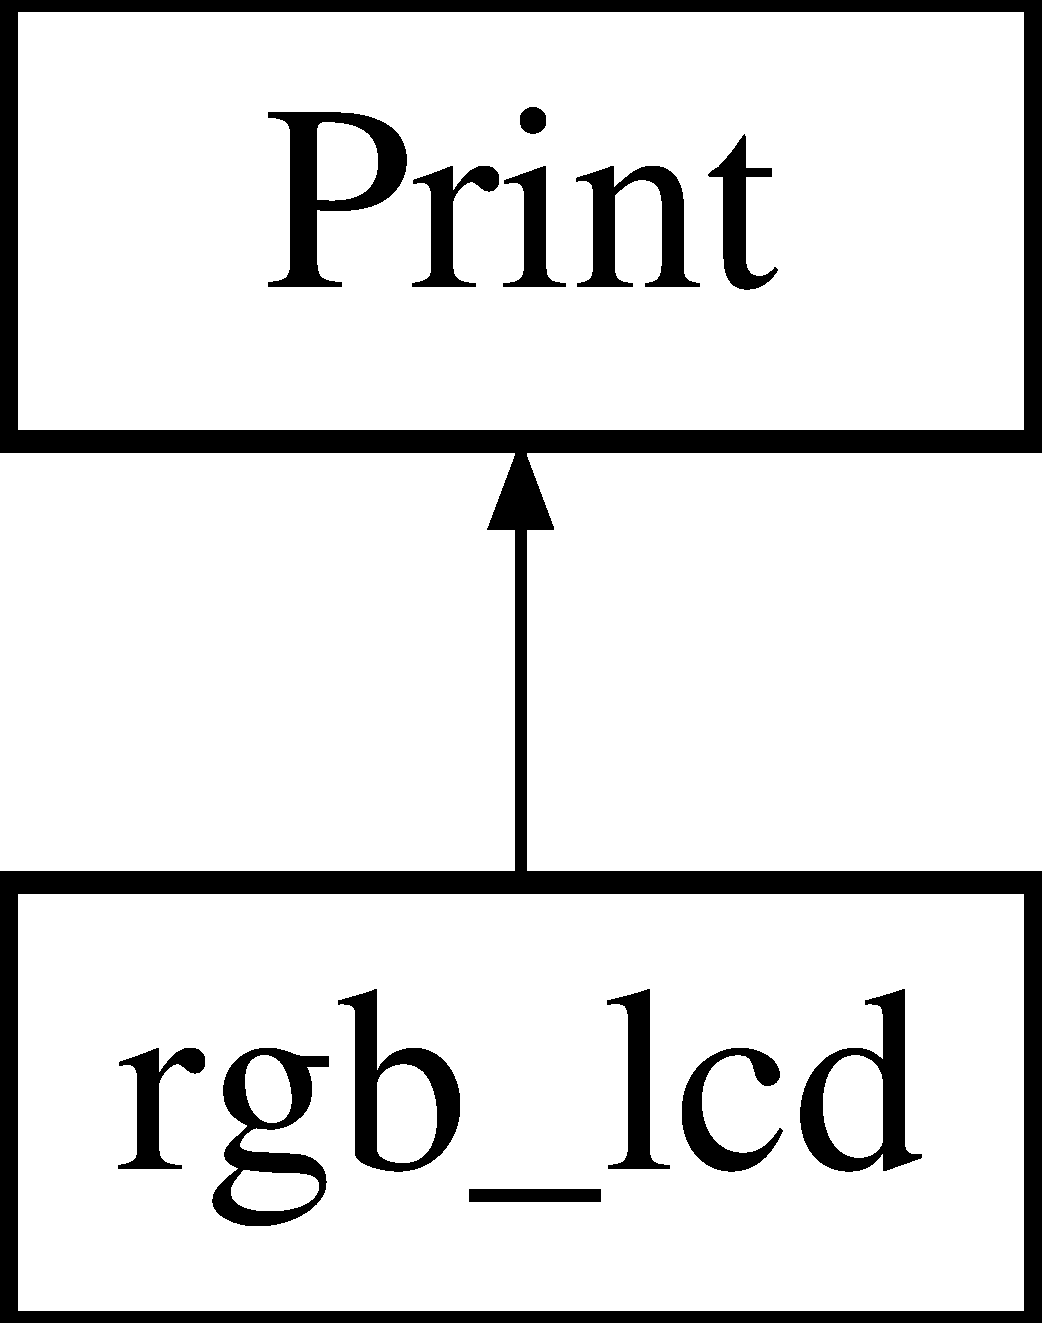
\includegraphics[height=2.000000cm]{classrgb__lcd}
\end{center}
\end{figure}
\subsection*{Public Member Functions}
\begin{DoxyCompactItemize}
\item 
\hyperlink{classrgb__lcd_ac651f214e977bc15e4f4f4bfc921ae6a}{rgb\+\_\+lcd} ()
\item 
void \hyperlink{classrgb__lcd_a828ec16645effff091b11356de90f016}{begin} (uint8\+\_\+t cols, uint8\+\_\+t rows, uint8\+\_\+t charsize=\hyperlink{rgb__lcd_8h_a9ef57e724c1b846dae0f531aff6fb464}{L\+C\+D\+\_\+5x8\+D\+O\+T\+S})
\item 
void \hyperlink{classrgb__lcd_a3be1a6075d03e10beff572c7303d6205}{clear} ()
\item 
void \hyperlink{classrgb__lcd_a3cb99ab37a932a7279605033a1f3627a}{home} ()
\item 
void \hyperlink{classrgb__lcd_ae74196f203857b5a0886668263cb6b0a}{no\+Display} ()
\item 
void \hyperlink{classrgb__lcd_aaa29ca8413bdc5e558f2f24575a0884b}{display} ()
\item 
void \hyperlink{classrgb__lcd_a2da54a37f1f57cec4f41a6f9415b278b}{no\+Blink} ()
\item 
void \hyperlink{classrgb__lcd_a9d7a1aca56d3b677eac640909e44317c}{blink} ()
\item 
void \hyperlink{classrgb__lcd_afcfef50ded29ec34468e56c1a578ad39}{no\+Cursor} ()
\item 
void \hyperlink{classrgb__lcd_a624fa4814b8d8e328cbaa1e030c7e5b6}{cursor} ()
\item 
void \hyperlink{classrgb__lcd_a13ec4ba249962dfa70e2296cbbbb59b7}{scroll\+Display\+Left} ()
\item 
void \hyperlink{classrgb__lcd_acba95981c737747a2bbf74698145dc85}{scroll\+Display\+Right} ()
\item 
void \hyperlink{classrgb__lcd_aa6a10cee260f41c76fc3ec76797ae3e1}{left\+To\+Right} ()
\item 
void \hyperlink{classrgb__lcd_ad023821ee7042a6c9602741febda6db6}{right\+To\+Left} ()
\item 
void \hyperlink{classrgb__lcd_a6280037a96fa1f40c3cc447e8c548076}{autoscroll} ()
\item 
void \hyperlink{classrgb__lcd_acda0feac43a242781f72e21e6f474d50}{no\+Autoscroll} ()
\item 
void \hyperlink{classrgb__lcd_a2904b44e55a03d5ae11d2dd1e940725e}{create\+Char} (uint8\+\_\+t, uint8\+\_\+t\mbox{[}$\,$\mbox{]})
\item 
void \hyperlink{classrgb__lcd_af4fb51c7b2dc73c4bad4ff3c54d808d5}{set\+Cursor} (uint8\+\_\+t, uint8\+\_\+t)
\item 
virtual size\+\_\+t \hyperlink{classrgb__lcd_afb79c9b7461d192545808de0555aa94c}{write} (uint8\+\_\+t)
\item 
void \hyperlink{classrgb__lcd_a4fadb9289928d7111636d006f47912de}{command} (uint8\+\_\+t)
\item 
void \hyperlink{classrgb__lcd_aa319b6f0ace80a28b1f3826f9fb0a1d5}{set\+R\+G\+B} (unsigned char r, unsigned char g, unsigned char b)
\item 
void \hyperlink{classrgb__lcd_aca034d77eb07e553d31ccab21014b5b7}{set\+P\+W\+M} (unsigned char color, unsigned char pwm)
\item 
void \hyperlink{classrgb__lcd_a2cc888d679923f959d2a2f19d2ca8519}{set\+Color} (unsigned char color)
\item 
void \hyperlink{classrgb__lcd_a9b57c5c6acf822fe86c2206bbf86d429}{set\+Color\+All} ()
\item 
void \hyperlink{classrgb__lcd_af90f303c88c594c27983f100b01960d3}{set\+Color\+White} ()
\end{DoxyCompactItemize}


\subsection{Constructor \& Destructor Documentation}
\hypertarget{classrgb__lcd_ac651f214e977bc15e4f4f4bfc921ae6a}{}\index{rgb\+\_\+lcd@{rgb\+\_\+lcd}!rgb\+\_\+lcd@{rgb\+\_\+lcd}}
\index{rgb\+\_\+lcd@{rgb\+\_\+lcd}!rgb\+\_\+lcd@{rgb\+\_\+lcd}}
\subsubsection[{rgb\+\_\+lcd}]{\setlength{\rightskip}{0pt plus 5cm}rgb\+\_\+lcd\+::rgb\+\_\+lcd (
\begin{DoxyParamCaption}
{}
\end{DoxyParamCaption}
)}\label{classrgb__lcd_ac651f214e977bc15e4f4f4bfc921ae6a}


\subsection{Member Function Documentation}
\hypertarget{classrgb__lcd_a6280037a96fa1f40c3cc447e8c548076}{}\index{rgb\+\_\+lcd@{rgb\+\_\+lcd}!autoscroll@{autoscroll}}
\index{autoscroll@{autoscroll}!rgb\+\_\+lcd@{rgb\+\_\+lcd}}
\subsubsection[{autoscroll}]{\setlength{\rightskip}{0pt plus 5cm}void rgb\+\_\+lcd\+::autoscroll (
\begin{DoxyParamCaption}
\item[{void}]{}
\end{DoxyParamCaption}
)}\label{classrgb__lcd_a6280037a96fa1f40c3cc447e8c548076}
\hypertarget{classrgb__lcd_a828ec16645effff091b11356de90f016}{}\index{rgb\+\_\+lcd@{rgb\+\_\+lcd}!begin@{begin}}
\index{begin@{begin}!rgb\+\_\+lcd@{rgb\+\_\+lcd}}
\subsubsection[{begin}]{\setlength{\rightskip}{0pt plus 5cm}void rgb\+\_\+lcd\+::begin (
\begin{DoxyParamCaption}
\item[{uint8\+\_\+t}]{cols, }
\item[{uint8\+\_\+t}]{rows, }
\item[{uint8\+\_\+t}]{charsize = {\ttfamily {\bf L\+C\+D\+\_\+5x8\+D\+O\+T\+S}}}
\end{DoxyParamCaption}
)}\label{classrgb__lcd_a828ec16645effff091b11356de90f016}
\hypertarget{classrgb__lcd_a9d7a1aca56d3b677eac640909e44317c}{}\index{rgb\+\_\+lcd@{rgb\+\_\+lcd}!blink@{blink}}
\index{blink@{blink}!rgb\+\_\+lcd@{rgb\+\_\+lcd}}
\subsubsection[{blink}]{\setlength{\rightskip}{0pt plus 5cm}void rgb\+\_\+lcd\+::blink (
\begin{DoxyParamCaption}
{}
\end{DoxyParamCaption}
)}\label{classrgb__lcd_a9d7a1aca56d3b677eac640909e44317c}
\hypertarget{classrgb__lcd_a3be1a6075d03e10beff572c7303d6205}{}\index{rgb\+\_\+lcd@{rgb\+\_\+lcd}!clear@{clear}}
\index{clear@{clear}!rgb\+\_\+lcd@{rgb\+\_\+lcd}}
\subsubsection[{clear}]{\setlength{\rightskip}{0pt plus 5cm}void rgb\+\_\+lcd\+::clear (
\begin{DoxyParamCaption}
{}
\end{DoxyParamCaption}
)}\label{classrgb__lcd_a3be1a6075d03e10beff572c7303d6205}
\hypertarget{classrgb__lcd_a4fadb9289928d7111636d006f47912de}{}\index{rgb\+\_\+lcd@{rgb\+\_\+lcd}!command@{command}}
\index{command@{command}!rgb\+\_\+lcd@{rgb\+\_\+lcd}}
\subsubsection[{command}]{\setlength{\rightskip}{0pt plus 5cm}void rgb\+\_\+lcd\+::command (
\begin{DoxyParamCaption}
\item[{uint8\+\_\+t}]{value}
\end{DoxyParamCaption}
)\hspace{0.3cm}{\ttfamily [inline]}}\label{classrgb__lcd_a4fadb9289928d7111636d006f47912de}
\hypertarget{classrgb__lcd_a2904b44e55a03d5ae11d2dd1e940725e}{}\index{rgb\+\_\+lcd@{rgb\+\_\+lcd}!create\+Char@{create\+Char}}
\index{create\+Char@{create\+Char}!rgb\+\_\+lcd@{rgb\+\_\+lcd}}
\subsubsection[{create\+Char}]{\setlength{\rightskip}{0pt plus 5cm}void rgb\+\_\+lcd\+::create\+Char (
\begin{DoxyParamCaption}
\item[{uint8\+\_\+t}]{location, }
\item[{uint8\+\_\+t}]{charmap\mbox{[}$\,$\mbox{]}}
\end{DoxyParamCaption}
)}\label{classrgb__lcd_a2904b44e55a03d5ae11d2dd1e940725e}
\hypertarget{classrgb__lcd_a624fa4814b8d8e328cbaa1e030c7e5b6}{}\index{rgb\+\_\+lcd@{rgb\+\_\+lcd}!cursor@{cursor}}
\index{cursor@{cursor}!rgb\+\_\+lcd@{rgb\+\_\+lcd}}
\subsubsection[{cursor}]{\setlength{\rightskip}{0pt plus 5cm}void rgb\+\_\+lcd\+::cursor (
\begin{DoxyParamCaption}
{}
\end{DoxyParamCaption}
)}\label{classrgb__lcd_a624fa4814b8d8e328cbaa1e030c7e5b6}
\hypertarget{classrgb__lcd_aaa29ca8413bdc5e558f2f24575a0884b}{}\index{rgb\+\_\+lcd@{rgb\+\_\+lcd}!display@{display}}
\index{display@{display}!rgb\+\_\+lcd@{rgb\+\_\+lcd}}
\subsubsection[{display}]{\setlength{\rightskip}{0pt plus 5cm}void rgb\+\_\+lcd\+::display (
\begin{DoxyParamCaption}
{}
\end{DoxyParamCaption}
)}\label{classrgb__lcd_aaa29ca8413bdc5e558f2f24575a0884b}
\hypertarget{classrgb__lcd_a3cb99ab37a932a7279605033a1f3627a}{}\index{rgb\+\_\+lcd@{rgb\+\_\+lcd}!home@{home}}
\index{home@{home}!rgb\+\_\+lcd@{rgb\+\_\+lcd}}
\subsubsection[{home}]{\setlength{\rightskip}{0pt plus 5cm}void rgb\+\_\+lcd\+::home (
\begin{DoxyParamCaption}
{}
\end{DoxyParamCaption}
)}\label{classrgb__lcd_a3cb99ab37a932a7279605033a1f3627a}
\hypertarget{classrgb__lcd_aa6a10cee260f41c76fc3ec76797ae3e1}{}\index{rgb\+\_\+lcd@{rgb\+\_\+lcd}!left\+To\+Right@{left\+To\+Right}}
\index{left\+To\+Right@{left\+To\+Right}!rgb\+\_\+lcd@{rgb\+\_\+lcd}}
\subsubsection[{left\+To\+Right}]{\setlength{\rightskip}{0pt plus 5cm}void rgb\+\_\+lcd\+::left\+To\+Right (
\begin{DoxyParamCaption}
\item[{void}]{}
\end{DoxyParamCaption}
)}\label{classrgb__lcd_aa6a10cee260f41c76fc3ec76797ae3e1}
\hypertarget{classrgb__lcd_acda0feac43a242781f72e21e6f474d50}{}\index{rgb\+\_\+lcd@{rgb\+\_\+lcd}!no\+Autoscroll@{no\+Autoscroll}}
\index{no\+Autoscroll@{no\+Autoscroll}!rgb\+\_\+lcd@{rgb\+\_\+lcd}}
\subsubsection[{no\+Autoscroll}]{\setlength{\rightskip}{0pt plus 5cm}void rgb\+\_\+lcd\+::no\+Autoscroll (
\begin{DoxyParamCaption}
\item[{void}]{}
\end{DoxyParamCaption}
)}\label{classrgb__lcd_acda0feac43a242781f72e21e6f474d50}
\hypertarget{classrgb__lcd_a2da54a37f1f57cec4f41a6f9415b278b}{}\index{rgb\+\_\+lcd@{rgb\+\_\+lcd}!no\+Blink@{no\+Blink}}
\index{no\+Blink@{no\+Blink}!rgb\+\_\+lcd@{rgb\+\_\+lcd}}
\subsubsection[{no\+Blink}]{\setlength{\rightskip}{0pt plus 5cm}void rgb\+\_\+lcd\+::no\+Blink (
\begin{DoxyParamCaption}
{}
\end{DoxyParamCaption}
)}\label{classrgb__lcd_a2da54a37f1f57cec4f41a6f9415b278b}
\hypertarget{classrgb__lcd_afcfef50ded29ec34468e56c1a578ad39}{}\index{rgb\+\_\+lcd@{rgb\+\_\+lcd}!no\+Cursor@{no\+Cursor}}
\index{no\+Cursor@{no\+Cursor}!rgb\+\_\+lcd@{rgb\+\_\+lcd}}
\subsubsection[{no\+Cursor}]{\setlength{\rightskip}{0pt plus 5cm}void rgb\+\_\+lcd\+::no\+Cursor (
\begin{DoxyParamCaption}
{}
\end{DoxyParamCaption}
)}\label{classrgb__lcd_afcfef50ded29ec34468e56c1a578ad39}
\hypertarget{classrgb__lcd_ae74196f203857b5a0886668263cb6b0a}{}\index{rgb\+\_\+lcd@{rgb\+\_\+lcd}!no\+Display@{no\+Display}}
\index{no\+Display@{no\+Display}!rgb\+\_\+lcd@{rgb\+\_\+lcd}}
\subsubsection[{no\+Display}]{\setlength{\rightskip}{0pt plus 5cm}void rgb\+\_\+lcd\+::no\+Display (
\begin{DoxyParamCaption}
{}
\end{DoxyParamCaption}
)}\label{classrgb__lcd_ae74196f203857b5a0886668263cb6b0a}
\hypertarget{classrgb__lcd_ad023821ee7042a6c9602741febda6db6}{}\index{rgb\+\_\+lcd@{rgb\+\_\+lcd}!right\+To\+Left@{right\+To\+Left}}
\index{right\+To\+Left@{right\+To\+Left}!rgb\+\_\+lcd@{rgb\+\_\+lcd}}
\subsubsection[{right\+To\+Left}]{\setlength{\rightskip}{0pt plus 5cm}void rgb\+\_\+lcd\+::right\+To\+Left (
\begin{DoxyParamCaption}
\item[{void}]{}
\end{DoxyParamCaption}
)}\label{classrgb__lcd_ad023821ee7042a6c9602741febda6db6}
\hypertarget{classrgb__lcd_a13ec4ba249962dfa70e2296cbbbb59b7}{}\index{rgb\+\_\+lcd@{rgb\+\_\+lcd}!scroll\+Display\+Left@{scroll\+Display\+Left}}
\index{scroll\+Display\+Left@{scroll\+Display\+Left}!rgb\+\_\+lcd@{rgb\+\_\+lcd}}
\subsubsection[{scroll\+Display\+Left}]{\setlength{\rightskip}{0pt plus 5cm}void rgb\+\_\+lcd\+::scroll\+Display\+Left (
\begin{DoxyParamCaption}
\item[{void}]{}
\end{DoxyParamCaption}
)}\label{classrgb__lcd_a13ec4ba249962dfa70e2296cbbbb59b7}
\hypertarget{classrgb__lcd_acba95981c737747a2bbf74698145dc85}{}\index{rgb\+\_\+lcd@{rgb\+\_\+lcd}!scroll\+Display\+Right@{scroll\+Display\+Right}}
\index{scroll\+Display\+Right@{scroll\+Display\+Right}!rgb\+\_\+lcd@{rgb\+\_\+lcd}}
\subsubsection[{scroll\+Display\+Right}]{\setlength{\rightskip}{0pt plus 5cm}void rgb\+\_\+lcd\+::scroll\+Display\+Right (
\begin{DoxyParamCaption}
\item[{void}]{}
\end{DoxyParamCaption}
)}\label{classrgb__lcd_acba95981c737747a2bbf74698145dc85}
\hypertarget{classrgb__lcd_a2cc888d679923f959d2a2f19d2ca8519}{}\index{rgb\+\_\+lcd@{rgb\+\_\+lcd}!set\+Color@{set\+Color}}
\index{set\+Color@{set\+Color}!rgb\+\_\+lcd@{rgb\+\_\+lcd}}
\subsubsection[{set\+Color}]{\setlength{\rightskip}{0pt plus 5cm}void rgb\+\_\+lcd\+::set\+Color (
\begin{DoxyParamCaption}
\item[{unsigned char}]{color}
\end{DoxyParamCaption}
)}\label{classrgb__lcd_a2cc888d679923f959d2a2f19d2ca8519}
\hypertarget{classrgb__lcd_a9b57c5c6acf822fe86c2206bbf86d429}{}\index{rgb\+\_\+lcd@{rgb\+\_\+lcd}!set\+Color\+All@{set\+Color\+All}}
\index{set\+Color\+All@{set\+Color\+All}!rgb\+\_\+lcd@{rgb\+\_\+lcd}}
\subsubsection[{set\+Color\+All}]{\setlength{\rightskip}{0pt plus 5cm}void rgb\+\_\+lcd\+::set\+Color\+All (
\begin{DoxyParamCaption}
{}
\end{DoxyParamCaption}
)\hspace{0.3cm}{\ttfamily [inline]}}\label{classrgb__lcd_a9b57c5c6acf822fe86c2206bbf86d429}
\hypertarget{classrgb__lcd_af90f303c88c594c27983f100b01960d3}{}\index{rgb\+\_\+lcd@{rgb\+\_\+lcd}!set\+Color\+White@{set\+Color\+White}}
\index{set\+Color\+White@{set\+Color\+White}!rgb\+\_\+lcd@{rgb\+\_\+lcd}}
\subsubsection[{set\+Color\+White}]{\setlength{\rightskip}{0pt plus 5cm}void rgb\+\_\+lcd\+::set\+Color\+White (
\begin{DoxyParamCaption}
{}
\end{DoxyParamCaption}
)\hspace{0.3cm}{\ttfamily [inline]}}\label{classrgb__lcd_af90f303c88c594c27983f100b01960d3}
\hypertarget{classrgb__lcd_af4fb51c7b2dc73c4bad4ff3c54d808d5}{}\index{rgb\+\_\+lcd@{rgb\+\_\+lcd}!set\+Cursor@{set\+Cursor}}
\index{set\+Cursor@{set\+Cursor}!rgb\+\_\+lcd@{rgb\+\_\+lcd}}
\subsubsection[{set\+Cursor}]{\setlength{\rightskip}{0pt plus 5cm}void rgb\+\_\+lcd\+::set\+Cursor (
\begin{DoxyParamCaption}
\item[{uint8\+\_\+t}]{col, }
\item[{uint8\+\_\+t}]{row}
\end{DoxyParamCaption}
)}\label{classrgb__lcd_af4fb51c7b2dc73c4bad4ff3c54d808d5}
\hypertarget{classrgb__lcd_aca034d77eb07e553d31ccab21014b5b7}{}\index{rgb\+\_\+lcd@{rgb\+\_\+lcd}!set\+P\+W\+M@{set\+P\+W\+M}}
\index{set\+P\+W\+M@{set\+P\+W\+M}!rgb\+\_\+lcd@{rgb\+\_\+lcd}}
\subsubsection[{set\+P\+W\+M}]{\setlength{\rightskip}{0pt plus 5cm}void rgb\+\_\+lcd\+::set\+P\+W\+M (
\begin{DoxyParamCaption}
\item[{unsigned char}]{color, }
\item[{unsigned char}]{pwm}
\end{DoxyParamCaption}
)\hspace{0.3cm}{\ttfamily [inline]}}\label{classrgb__lcd_aca034d77eb07e553d31ccab21014b5b7}
\hypertarget{classrgb__lcd_aa319b6f0ace80a28b1f3826f9fb0a1d5}{}\index{rgb\+\_\+lcd@{rgb\+\_\+lcd}!set\+R\+G\+B@{set\+R\+G\+B}}
\index{set\+R\+G\+B@{set\+R\+G\+B}!rgb\+\_\+lcd@{rgb\+\_\+lcd}}
\subsubsection[{set\+R\+G\+B}]{\setlength{\rightskip}{0pt plus 5cm}void rgb\+\_\+lcd\+::set\+R\+G\+B (
\begin{DoxyParamCaption}
\item[{unsigned char}]{r, }
\item[{unsigned char}]{g, }
\item[{unsigned char}]{b}
\end{DoxyParamCaption}
)}\label{classrgb__lcd_aa319b6f0ace80a28b1f3826f9fb0a1d5}
\hypertarget{classrgb__lcd_afb79c9b7461d192545808de0555aa94c}{}\index{rgb\+\_\+lcd@{rgb\+\_\+lcd}!write@{write}}
\index{write@{write}!rgb\+\_\+lcd@{rgb\+\_\+lcd}}
\subsubsection[{write}]{\setlength{\rightskip}{0pt plus 5cm}size\+\_\+t rgb\+\_\+lcd\+::write (
\begin{DoxyParamCaption}
\item[{uint8\+\_\+t}]{value}
\end{DoxyParamCaption}
)\hspace{0.3cm}{\ttfamily [inline]}, {\ttfamily [virtual]}}\label{classrgb__lcd_afb79c9b7461d192545808de0555aa94c}


The documentation for this class was generated from the following files\+:\begin{DoxyCompactItemize}
\item 
\hyperlink{rgb__lcd_8h}{rgb\+\_\+lcd.\+h}\item 
\hyperlink{rgb__lcd_8cpp}{rgb\+\_\+lcd.\+cpp}\end{DoxyCompactItemize}

\hypertarget{class_sensor_contact_switch}{}\section{Sensor\+Contact\+Switch Class Reference}
\label{class_sensor_contact_switch}\index{Sensor\+Contact\+Switch@{Sensor\+Contact\+Switch}}


{\ttfamily \#include $<$sensor\+\_\+contact\+\_\+switch.\+h$>$}

\subsection*{Public Member Functions}
\begin{DoxyCompactItemize}
\item 
\hyperlink{class_sensor_contact_switch_a821878d797ea7b94dd2870f98df8fdf5}{Sensor\+Contact\+Switch} (int pin, String instruction\+\_\+code, int instruction\+\_\+id)
\item 
void \hyperlink{class_sensor_contact_switch_a037d866b1e40776cc6fa00a46169b150}{begin} (void)
\item 
String \hyperlink{class_sensor_contact_switch_a99a5906b45ed441eea56fb2960d35191}{get} (void)
\item 
String \hyperlink{class_sensor_contact_switch_ab49acd5d6132eed50d7342717649abc2}{set} (String instruction\+\_\+code, int instruction\+\_\+id, String instruction\+\_\+parameter)
\end{DoxyCompactItemize}
\subsection*{Public Attributes}
\begin{DoxyCompactItemize}
\item 
bool \hyperlink{class_sensor_contact_switch_a38d5bad22015b2013e776dec61bc8622}{is\+\_\+connected\+\_\+}
\end{DoxyCompactItemize}


\subsection{Constructor \& Destructor Documentation}
\hypertarget{class_sensor_contact_switch_a821878d797ea7b94dd2870f98df8fdf5}{}\index{Sensor\+Contact\+Switch@{Sensor\+Contact\+Switch}!Sensor\+Contact\+Switch@{Sensor\+Contact\+Switch}}
\index{Sensor\+Contact\+Switch@{Sensor\+Contact\+Switch}!Sensor\+Contact\+Switch@{Sensor\+Contact\+Switch}}
\subsubsection[{Sensor\+Contact\+Switch}]{\setlength{\rightskip}{0pt plus 5cm}Sensor\+Contact\+Switch\+::\+Sensor\+Contact\+Switch (
\begin{DoxyParamCaption}
\item[{int}]{pin, }
\item[{String}]{instruction\+\_\+code, }
\item[{int}]{instruction\+\_\+id}
\end{DoxyParamCaption}
)}\label{class_sensor_contact_switch_a821878d797ea7b94dd2870f98df8fdf5}


\subsection{Member Function Documentation}
\hypertarget{class_sensor_contact_switch_a037d866b1e40776cc6fa00a46169b150}{}\index{Sensor\+Contact\+Switch@{Sensor\+Contact\+Switch}!begin@{begin}}
\index{begin@{begin}!Sensor\+Contact\+Switch@{Sensor\+Contact\+Switch}}
\subsubsection[{begin}]{\setlength{\rightskip}{0pt plus 5cm}void Sensor\+Contact\+Switch\+::begin (
\begin{DoxyParamCaption}
\item[{void}]{}
\end{DoxyParamCaption}
)}\label{class_sensor_contact_switch_a037d866b1e40776cc6fa00a46169b150}
\hypertarget{class_sensor_contact_switch_a99a5906b45ed441eea56fb2960d35191}{}\index{Sensor\+Contact\+Switch@{Sensor\+Contact\+Switch}!get@{get}}
\index{get@{get}!Sensor\+Contact\+Switch@{Sensor\+Contact\+Switch}}
\subsubsection[{get}]{\setlength{\rightskip}{0pt plus 5cm}String Sensor\+Contact\+Switch\+::get (
\begin{DoxyParamCaption}
\item[{void}]{}
\end{DoxyParamCaption}
)}\label{class_sensor_contact_switch_a99a5906b45ed441eea56fb2960d35191}
\hypertarget{class_sensor_contact_switch_ab49acd5d6132eed50d7342717649abc2}{}\index{Sensor\+Contact\+Switch@{Sensor\+Contact\+Switch}!set@{set}}
\index{set@{set}!Sensor\+Contact\+Switch@{Sensor\+Contact\+Switch}}
\subsubsection[{set}]{\setlength{\rightskip}{0pt plus 5cm}String Sensor\+Contact\+Switch\+::set (
\begin{DoxyParamCaption}
\item[{String}]{instruction\+\_\+code, }
\item[{int}]{instruction\+\_\+id, }
\item[{String}]{instruction\+\_\+parameter}
\end{DoxyParamCaption}
)}\label{class_sensor_contact_switch_ab49acd5d6132eed50d7342717649abc2}


\subsection{Member Data Documentation}
\hypertarget{class_sensor_contact_switch_a38d5bad22015b2013e776dec61bc8622}{}\index{Sensor\+Contact\+Switch@{Sensor\+Contact\+Switch}!is\+\_\+connected\+\_\+@{is\+\_\+connected\+\_\+}}
\index{is\+\_\+connected\+\_\+@{is\+\_\+connected\+\_\+}!Sensor\+Contact\+Switch@{Sensor\+Contact\+Switch}}
\subsubsection[{is\+\_\+connected\+\_\+}]{\setlength{\rightskip}{0pt plus 5cm}bool Sensor\+Contact\+Switch\+::is\+\_\+connected\+\_\+}\label{class_sensor_contact_switch_a38d5bad22015b2013e776dec61bc8622}


The documentation for this class was generated from the following files\+:\begin{DoxyCompactItemize}
\item 
\hyperlink{sensor__contact__switch_8h}{sensor\+\_\+contact\+\_\+switch.\+h}\item 
\hyperlink{sensor__contact__switch_8cpp}{sensor\+\_\+contact\+\_\+switch.\+cpp}\end{DoxyCompactItemize}

\hypertarget{class_sensor_dfr0161}{}\section{Sensor\+Dfr0161 Class Reference}
\label{class_sensor_dfr0161}\index{Sensor\+Dfr0161@{Sensor\+Dfr0161}}


{\ttfamily \#include $<$sensor\+\_\+dfr0161.\+h$>$}

\subsection*{Public Member Functions}
\begin{DoxyCompactItemize}
\item 
\hyperlink{class_sensor_dfr0161_a2610eb178b9cd0c2e00738df72863e8b}{Sensor\+Dfr0161} (uint8\+\_\+t ph\+\_\+pin, String ph\+\_\+instruction\+\_\+code, int ph\+\_\+instruction\+\_\+id)
\item 
void \hyperlink{class_sensor_dfr0161_aee10a8faa4f752486a3a14662ba70d2d}{begin} (void)
\item 
String \hyperlink{class_sensor_dfr0161_a85017ddaf1e4ef3c09ea77fd0625e691}{get} (void)
\item 
String \hyperlink{class_sensor_dfr0161_a072cbfa3e18f9e5dd7b2faeec20721c3}{set} (String ph\+\_\+instruction\+\_\+code, int ph\+\_\+instruction\+\_\+id, String pg\+\_\+instruction\+\_\+parameter)
\item 
double \hyperlink{class_sensor_dfr0161_a659010048f28fd711b98a29b7825486f}{get\+Ph} (void)
\end{DoxyCompactItemize}
\subsection*{Public Attributes}
\begin{DoxyCompactItemize}
\item 
float \hyperlink{class_sensor_dfr0161_a98640420a5bd5b7461341893c1a8633b}{ph}
\item 
float \hyperlink{class_sensor_dfr0161_a84060ac1d68a19d8cbc7505484c31391}{ph\+\_\+avg}
\end{DoxyCompactItemize}


\subsection{Constructor \& Destructor Documentation}
\hypertarget{class_sensor_dfr0161_a2610eb178b9cd0c2e00738df72863e8b}{}\index{Sensor\+Dfr0161@{Sensor\+Dfr0161}!Sensor\+Dfr0161@{Sensor\+Dfr0161}}
\index{Sensor\+Dfr0161@{Sensor\+Dfr0161}!Sensor\+Dfr0161@{Sensor\+Dfr0161}}
\subsubsection[{Sensor\+Dfr0161}]{\setlength{\rightskip}{0pt plus 5cm}Sensor\+Dfr0161\+::\+Sensor\+Dfr0161 (
\begin{DoxyParamCaption}
\item[{uint8\+\_\+t}]{ph\+\_\+pin, }
\item[{String}]{ph\+\_\+instruction\+\_\+code, }
\item[{int}]{ph\+\_\+instruction\+\_\+id}
\end{DoxyParamCaption}
)}\label{class_sensor_dfr0161_a2610eb178b9cd0c2e00738df72863e8b}


\subsection{Member Function Documentation}
\hypertarget{class_sensor_dfr0161_aee10a8faa4f752486a3a14662ba70d2d}{}\index{Sensor\+Dfr0161@{Sensor\+Dfr0161}!begin@{begin}}
\index{begin@{begin}!Sensor\+Dfr0161@{Sensor\+Dfr0161}}
\subsubsection[{begin}]{\setlength{\rightskip}{0pt plus 5cm}void Sensor\+Dfr0161\+::begin (
\begin{DoxyParamCaption}
\item[{void}]{}
\end{DoxyParamCaption}
)}\label{class_sensor_dfr0161_aee10a8faa4f752486a3a14662ba70d2d}
\hypertarget{class_sensor_dfr0161_a85017ddaf1e4ef3c09ea77fd0625e691}{}\index{Sensor\+Dfr0161@{Sensor\+Dfr0161}!get@{get}}
\index{get@{get}!Sensor\+Dfr0161@{Sensor\+Dfr0161}}
\subsubsection[{get}]{\setlength{\rightskip}{0pt plus 5cm}String Sensor\+Dfr0161\+::get (
\begin{DoxyParamCaption}
\item[{void}]{}
\end{DoxyParamCaption}
)}\label{class_sensor_dfr0161_a85017ddaf1e4ef3c09ea77fd0625e691}
\hypertarget{class_sensor_dfr0161_a659010048f28fd711b98a29b7825486f}{}\index{Sensor\+Dfr0161@{Sensor\+Dfr0161}!get\+Ph@{get\+Ph}}
\index{get\+Ph@{get\+Ph}!Sensor\+Dfr0161@{Sensor\+Dfr0161}}
\subsubsection[{get\+Ph}]{\setlength{\rightskip}{0pt plus 5cm}double Sensor\+Dfr0161\+::get\+Ph (
\begin{DoxyParamCaption}
\item[{void}]{}
\end{DoxyParamCaption}
)}\label{class_sensor_dfr0161_a659010048f28fd711b98a29b7825486f}
\hypertarget{class_sensor_dfr0161_a072cbfa3e18f9e5dd7b2faeec20721c3}{}\index{Sensor\+Dfr0161@{Sensor\+Dfr0161}!set@{set}}
\index{set@{set}!Sensor\+Dfr0161@{Sensor\+Dfr0161}}
\subsubsection[{set}]{\setlength{\rightskip}{0pt plus 5cm}String Sensor\+Dfr0161\+::set (
\begin{DoxyParamCaption}
\item[{String}]{ph\+\_\+instruction\+\_\+code, }
\item[{int}]{ph\+\_\+instruction\+\_\+id, }
\item[{String}]{pg\+\_\+instruction\+\_\+parameter}
\end{DoxyParamCaption}
)}\label{class_sensor_dfr0161_a072cbfa3e18f9e5dd7b2faeec20721c3}


\subsection{Member Data Documentation}
\hypertarget{class_sensor_dfr0161_a98640420a5bd5b7461341893c1a8633b}{}\index{Sensor\+Dfr0161@{Sensor\+Dfr0161}!ph@{ph}}
\index{ph@{ph}!Sensor\+Dfr0161@{Sensor\+Dfr0161}}
\subsubsection[{ph}]{\setlength{\rightskip}{0pt plus 5cm}float Sensor\+Dfr0161\+::ph}\label{class_sensor_dfr0161_a98640420a5bd5b7461341893c1a8633b}
\hypertarget{class_sensor_dfr0161_a84060ac1d68a19d8cbc7505484c31391}{}\index{Sensor\+Dfr0161@{Sensor\+Dfr0161}!ph\+\_\+avg@{ph\+\_\+avg}}
\index{ph\+\_\+avg@{ph\+\_\+avg}!Sensor\+Dfr0161@{Sensor\+Dfr0161}}
\subsubsection[{ph\+\_\+avg}]{\setlength{\rightskip}{0pt plus 5cm}float Sensor\+Dfr0161\+::ph\+\_\+avg}\label{class_sensor_dfr0161_a84060ac1d68a19d8cbc7505484c31391}


The documentation for this class was generated from the following files\+:\begin{DoxyCompactItemize}
\item 
\hyperlink{sensor__dfr0161_8h}{sensor\+\_\+dfr0161.\+h}\item 
\hyperlink{sensor__dfr0161_8cpp}{sensor\+\_\+dfr0161.\+cpp}\end{DoxyCompactItemize}

\hypertarget{class_sensor_dfr0300}{}\section{Sensor\+Dfr0300 Class Reference}
\label{class_sensor_dfr0300}\index{Sensor\+Dfr0300@{Sensor\+Dfr0300}}


{\ttfamily \#include $<$sensor\+\_\+dfr0300.\+h$>$}

\subsection*{Public Member Functions}
\begin{DoxyCompactItemize}
\item 
\hyperlink{class_sensor_dfr0300_a8a318afa69fd7aeb2c5d331bf3cc196a}{Sensor\+Dfr0300} (int temperature\+\_\+pin, int ec\+\_\+pin, int ec\+\_\+enable\+\_\+pin, String temperature\+\_\+instruction\+\_\+code, int temperature\+\_\+id, String ec\+\_\+instruction\+\_\+code, int ec\+\_\+id)
\item 
void \hyperlink{class_sensor_dfr0300_a310bf946e482b58ab079d43f3bb3093b}{begin} (void)
\item 
String \hyperlink{class_sensor_dfr0300_a16b2e1ab7ed6bd191ea3a4d588d28861}{get} (void)
\item 
String \hyperlink{class_sensor_dfr0300_a538a5bd7f86693ce975d4b4b7f48bee0}{set} (String instruction\+\_\+code, int instruction\+\_\+id, String instruction\+\_\+parameter)
\end{DoxyCompactItemize}
\subsection*{Public Attributes}
\begin{DoxyCompactItemize}
\item 
float \hyperlink{class_sensor_dfr0300_acc4191cfd71800c3aa571bcb1820b385}{temperature}
\item 
float \hyperlink{class_sensor_dfr0300_abe5609d68642bb1f9e898820dd742671}{ec}
\item 
float \hyperlink{class_sensor_dfr0300_a110d741893fd0fca0145325b3ffa8300}{ec\+\_\+avg}
\end{DoxyCompactItemize}


\subsection{Constructor \& Destructor Documentation}
\hypertarget{class_sensor_dfr0300_a8a318afa69fd7aeb2c5d331bf3cc196a}{}\index{Sensor\+Dfr0300@{Sensor\+Dfr0300}!Sensor\+Dfr0300@{Sensor\+Dfr0300}}
\index{Sensor\+Dfr0300@{Sensor\+Dfr0300}!Sensor\+Dfr0300@{Sensor\+Dfr0300}}
\subsubsection[{Sensor\+Dfr0300}]{\setlength{\rightskip}{0pt plus 5cm}Sensor\+Dfr0300\+::\+Sensor\+Dfr0300 (
\begin{DoxyParamCaption}
\item[{int}]{temperature\+\_\+pin, }
\item[{int}]{ec\+\_\+pin, }
\item[{int}]{ec\+\_\+enable\+\_\+pin, }
\item[{String}]{temperature\+\_\+instruction\+\_\+code, }
\item[{int}]{temperature\+\_\+id, }
\item[{String}]{ec\+\_\+instruction\+\_\+code, }
\item[{int}]{ec\+\_\+id}
\end{DoxyParamCaption}
)}\label{class_sensor_dfr0300_a8a318afa69fd7aeb2c5d331bf3cc196a}


\subsection{Member Function Documentation}
\hypertarget{class_sensor_dfr0300_a310bf946e482b58ab079d43f3bb3093b}{}\index{Sensor\+Dfr0300@{Sensor\+Dfr0300}!begin@{begin}}
\index{begin@{begin}!Sensor\+Dfr0300@{Sensor\+Dfr0300}}
\subsubsection[{begin}]{\setlength{\rightskip}{0pt plus 5cm}void Sensor\+Dfr0300\+::begin (
\begin{DoxyParamCaption}
\item[{void}]{}
\end{DoxyParamCaption}
)}\label{class_sensor_dfr0300_a310bf946e482b58ab079d43f3bb3093b}
\hypertarget{class_sensor_dfr0300_a16b2e1ab7ed6bd191ea3a4d588d28861}{}\index{Sensor\+Dfr0300@{Sensor\+Dfr0300}!get@{get}}
\index{get@{get}!Sensor\+Dfr0300@{Sensor\+Dfr0300}}
\subsubsection[{get}]{\setlength{\rightskip}{0pt plus 5cm}String Sensor\+Dfr0300\+::get (
\begin{DoxyParamCaption}
\item[{void}]{}
\end{DoxyParamCaption}
)}\label{class_sensor_dfr0300_a16b2e1ab7ed6bd191ea3a4d588d28861}
\hypertarget{class_sensor_dfr0300_a538a5bd7f86693ce975d4b4b7f48bee0}{}\index{Sensor\+Dfr0300@{Sensor\+Dfr0300}!set@{set}}
\index{set@{set}!Sensor\+Dfr0300@{Sensor\+Dfr0300}}
\subsubsection[{set}]{\setlength{\rightskip}{0pt plus 5cm}String Sensor\+Dfr0300\+::set (
\begin{DoxyParamCaption}
\item[{String}]{instruction\+\_\+code, }
\item[{int}]{instruction\+\_\+id, }
\item[{String}]{instruction\+\_\+parameter}
\end{DoxyParamCaption}
)}\label{class_sensor_dfr0300_a538a5bd7f86693ce975d4b4b7f48bee0}


\subsection{Member Data Documentation}
\hypertarget{class_sensor_dfr0300_abe5609d68642bb1f9e898820dd742671}{}\index{Sensor\+Dfr0300@{Sensor\+Dfr0300}!ec@{ec}}
\index{ec@{ec}!Sensor\+Dfr0300@{Sensor\+Dfr0300}}
\subsubsection[{ec}]{\setlength{\rightskip}{0pt plus 5cm}float Sensor\+Dfr0300\+::ec}\label{class_sensor_dfr0300_abe5609d68642bb1f9e898820dd742671}
\hypertarget{class_sensor_dfr0300_a110d741893fd0fca0145325b3ffa8300}{}\index{Sensor\+Dfr0300@{Sensor\+Dfr0300}!ec\+\_\+avg@{ec\+\_\+avg}}
\index{ec\+\_\+avg@{ec\+\_\+avg}!Sensor\+Dfr0300@{Sensor\+Dfr0300}}
\subsubsection[{ec\+\_\+avg}]{\setlength{\rightskip}{0pt plus 5cm}float Sensor\+Dfr0300\+::ec\+\_\+avg}\label{class_sensor_dfr0300_a110d741893fd0fca0145325b3ffa8300}
\hypertarget{class_sensor_dfr0300_acc4191cfd71800c3aa571bcb1820b385}{}\index{Sensor\+Dfr0300@{Sensor\+Dfr0300}!temperature@{temperature}}
\index{temperature@{temperature}!Sensor\+Dfr0300@{Sensor\+Dfr0300}}
\subsubsection[{temperature}]{\setlength{\rightskip}{0pt plus 5cm}float Sensor\+Dfr0300\+::temperature}\label{class_sensor_dfr0300_acc4191cfd71800c3aa571bcb1820b385}


The documentation for this class was generated from the following files\+:\begin{DoxyCompactItemize}
\item 
\hyperlink{sensor__dfr0300_8h}{sensor\+\_\+dfr0300.\+h}\item 
\hyperlink{sensor__dfr0300_8cpp}{sensor\+\_\+dfr0300.\+cpp}\end{DoxyCompactItemize}

\hypertarget{class_sensor_dht22}{}\section{Sensor\+Dht22 Class Reference}
\label{class_sensor_dht22}\index{Sensor\+Dht22@{Sensor\+Dht22}}


{\ttfamily \#include $<$sensor\+\_\+dht22.\+h$>$}

\subsection*{Public Member Functions}
\begin{DoxyCompactItemize}
\item 
\hyperlink{class_sensor_dht22_a417840f2a31737059e6b0885d89de32f}{Sensor\+Dht22} (int pin, String temperature\+\_\+instruction\+\_\+code, int temperature\+\_\+instruction\+\_\+id, String humidity\+\_\+instruction\+\_\+code, int humidity\+\_\+instruction\+\_\+id)
\item 
void \hyperlink{class_sensor_dht22_ae4de2976d82d060c9dc12bf84195a347}{begin} (void)
\item 
String \hyperlink{class_sensor_dht22_ad939eefeb967eea7029d9505cc6aad6f}{get} (void)
\item 
String \hyperlink{class_sensor_dht22_a177a42edbc33d5cf4fa0c4c38dc0047c}{set} (String instruction\+\_\+code, int instruction\+\_\+id, String parameter)
\end{DoxyCompactItemize}
\subsection*{Public Attributes}
\begin{DoxyCompactItemize}
\item 
float \hyperlink{class_sensor_dht22_a93f9363f3086e00f440fc89a7f1f8a1b}{humidity}
\item 
float \hyperlink{class_sensor_dht22_af35665067c66e887afa5fef5611fb48a}{temperature}
\end{DoxyCompactItemize}


\subsection{Constructor \& Destructor Documentation}
\hypertarget{class_sensor_dht22_a417840f2a31737059e6b0885d89de32f}{}\index{Sensor\+Dht22@{Sensor\+Dht22}!Sensor\+Dht22@{Sensor\+Dht22}}
\index{Sensor\+Dht22@{Sensor\+Dht22}!Sensor\+Dht22@{Sensor\+Dht22}}
\subsubsection[{Sensor\+Dht22}]{\setlength{\rightskip}{0pt plus 5cm}Sensor\+Dht22\+::\+Sensor\+Dht22 (
\begin{DoxyParamCaption}
\item[{int}]{pin, }
\item[{String}]{temperature\+\_\+instruction\+\_\+code, }
\item[{int}]{temperature\+\_\+instruction\+\_\+id, }
\item[{String}]{humidity\+\_\+instruction\+\_\+code, }
\item[{int}]{humidity\+\_\+instruction\+\_\+id}
\end{DoxyParamCaption}
)}\label{class_sensor_dht22_a417840f2a31737059e6b0885d89de32f}


\subsection{Member Function Documentation}
\hypertarget{class_sensor_dht22_ae4de2976d82d060c9dc12bf84195a347}{}\index{Sensor\+Dht22@{Sensor\+Dht22}!begin@{begin}}
\index{begin@{begin}!Sensor\+Dht22@{Sensor\+Dht22}}
\subsubsection[{begin}]{\setlength{\rightskip}{0pt plus 5cm}void Sensor\+Dht22\+::begin (
\begin{DoxyParamCaption}
\item[{void}]{}
\end{DoxyParamCaption}
)}\label{class_sensor_dht22_ae4de2976d82d060c9dc12bf84195a347}
\hypertarget{class_sensor_dht22_ad939eefeb967eea7029d9505cc6aad6f}{}\index{Sensor\+Dht22@{Sensor\+Dht22}!get@{get}}
\index{get@{get}!Sensor\+Dht22@{Sensor\+Dht22}}
\subsubsection[{get}]{\setlength{\rightskip}{0pt plus 5cm}String Sensor\+Dht22\+::get (
\begin{DoxyParamCaption}
\item[{void}]{}
\end{DoxyParamCaption}
)}\label{class_sensor_dht22_ad939eefeb967eea7029d9505cc6aad6f}
\hypertarget{class_sensor_dht22_a177a42edbc33d5cf4fa0c4c38dc0047c}{}\index{Sensor\+Dht22@{Sensor\+Dht22}!set@{set}}
\index{set@{set}!Sensor\+Dht22@{Sensor\+Dht22}}
\subsubsection[{set}]{\setlength{\rightskip}{0pt plus 5cm}String Sensor\+Dht22\+::set (
\begin{DoxyParamCaption}
\item[{String}]{instruction\+\_\+code, }
\item[{int}]{instruction\+\_\+id, }
\item[{String}]{parameter}
\end{DoxyParamCaption}
)}\label{class_sensor_dht22_a177a42edbc33d5cf4fa0c4c38dc0047c}


\subsection{Member Data Documentation}
\hypertarget{class_sensor_dht22_a93f9363f3086e00f440fc89a7f1f8a1b}{}\index{Sensor\+Dht22@{Sensor\+Dht22}!humidity@{humidity}}
\index{humidity@{humidity}!Sensor\+Dht22@{Sensor\+Dht22}}
\subsubsection[{humidity}]{\setlength{\rightskip}{0pt plus 5cm}float Sensor\+Dht22\+::humidity}\label{class_sensor_dht22_a93f9363f3086e00f440fc89a7f1f8a1b}
\hypertarget{class_sensor_dht22_af35665067c66e887afa5fef5611fb48a}{}\index{Sensor\+Dht22@{Sensor\+Dht22}!temperature@{temperature}}
\index{temperature@{temperature}!Sensor\+Dht22@{Sensor\+Dht22}}
\subsubsection[{temperature}]{\setlength{\rightskip}{0pt plus 5cm}float Sensor\+Dht22\+::temperature}\label{class_sensor_dht22_af35665067c66e887afa5fef5611fb48a}


The documentation for this class was generated from the following files\+:\begin{DoxyCompactItemize}
\item 
\hyperlink{sensor__dht22_8h}{sensor\+\_\+dht22.\+h}\item 
\hyperlink{sensor__dht22_8cpp}{sensor\+\_\+dht22.\+cpp}\end{DoxyCompactItemize}

\hypertarget{class_sensor_gc0011}{}\section{Sensor\+Gc0011 Class Reference}
\label{class_sensor_gc0011}\index{Sensor\+Gc0011@{Sensor\+Gc0011}}


{\ttfamily \#include $<$sensor\+\_\+gc0011.\+h$>$}

\subsection*{Public Member Functions}
\begin{DoxyCompactItemize}
\item 
\hyperlink{class_sensor_gc0011_ac8b12368b4b524198210048fbd1d0c81}{Sensor\+Gc0011} (int rx\+\_\+pin, int tx\+\_\+pin, String co2\+\_\+instruction\+\_\+code, int co2\+\_\+instruction\+\_\+id, String temperature\+\_\+instruction\+\_\+code, int temperature\+\_\+instruction\+\_\+id, String humidity\+\_\+instruction\+\_\+code, int humidity\+\_\+instruction\+\_\+id)
\item 
void \hyperlink{class_sensor_gc0011_a661743d47448c6b9c965fd8e1f123fbc}{begin} (void)
\item 
String \hyperlink{class_sensor_gc0011_a2920401f54e121bba1398d52e9b2c90a}{get} (void)
\item 
String \hyperlink{class_sensor_gc0011_a658b7856221577342b54e4dc7fe06d2a}{set} (String instruction\+\_\+code, int instruction\+\_\+id, String instruction\+\_\+parameter)
\end{DoxyCompactItemize}
\subsection*{Public Attributes}
\begin{DoxyCompactItemize}
\item 
float \hyperlink{class_sensor_gc0011_a6da77eb384ff77e28c2fa092a03a4cbb}{temperature}
\item 
float \hyperlink{class_sensor_gc0011_af5964ea62f030dd4ea2f219224afa4e6}{humidity}
\item 
float \hyperlink{class_sensor_gc0011_acd7c57373be1c5fb21c8da8c25861138}{co2}
\end{DoxyCompactItemize}


\subsection{Constructor \& Destructor Documentation}
\hypertarget{class_sensor_gc0011_ac8b12368b4b524198210048fbd1d0c81}{}\index{Sensor\+Gc0011@{Sensor\+Gc0011}!Sensor\+Gc0011@{Sensor\+Gc0011}}
\index{Sensor\+Gc0011@{Sensor\+Gc0011}!Sensor\+Gc0011@{Sensor\+Gc0011}}
\subsubsection[{Sensor\+Gc0011}]{\setlength{\rightskip}{0pt plus 5cm}Sensor\+Gc0011\+::\+Sensor\+Gc0011 (
\begin{DoxyParamCaption}
\item[{int}]{rx\+\_\+pin, }
\item[{int}]{tx\+\_\+pin, }
\item[{String}]{co2\+\_\+instruction\+\_\+code, }
\item[{int}]{co2\+\_\+instruction\+\_\+id, }
\item[{String}]{temperature\+\_\+instruction\+\_\+code, }
\item[{int}]{temperature\+\_\+instruction\+\_\+id, }
\item[{String}]{humidity\+\_\+instruction\+\_\+code, }
\item[{int}]{humidity\+\_\+instruction\+\_\+id}
\end{DoxyParamCaption}
)}\label{class_sensor_gc0011_ac8b12368b4b524198210048fbd1d0c81}


\subsection{Member Function Documentation}
\hypertarget{class_sensor_gc0011_a661743d47448c6b9c965fd8e1f123fbc}{}\index{Sensor\+Gc0011@{Sensor\+Gc0011}!begin@{begin}}
\index{begin@{begin}!Sensor\+Gc0011@{Sensor\+Gc0011}}
\subsubsection[{begin}]{\setlength{\rightskip}{0pt plus 5cm}void Sensor\+Gc0011\+::begin (
\begin{DoxyParamCaption}
\item[{void}]{}
\end{DoxyParamCaption}
)}\label{class_sensor_gc0011_a661743d47448c6b9c965fd8e1f123fbc}
\hypertarget{class_sensor_gc0011_a2920401f54e121bba1398d52e9b2c90a}{}\index{Sensor\+Gc0011@{Sensor\+Gc0011}!get@{get}}
\index{get@{get}!Sensor\+Gc0011@{Sensor\+Gc0011}}
\subsubsection[{get}]{\setlength{\rightskip}{0pt plus 5cm}String Sensor\+Gc0011\+::get (
\begin{DoxyParamCaption}
\item[{void}]{}
\end{DoxyParamCaption}
)}\label{class_sensor_gc0011_a2920401f54e121bba1398d52e9b2c90a}
\hypertarget{class_sensor_gc0011_a658b7856221577342b54e4dc7fe06d2a}{}\index{Sensor\+Gc0011@{Sensor\+Gc0011}!set@{set}}
\index{set@{set}!Sensor\+Gc0011@{Sensor\+Gc0011}}
\subsubsection[{set}]{\setlength{\rightskip}{0pt plus 5cm}String Sensor\+Gc0011\+::set (
\begin{DoxyParamCaption}
\item[{String}]{instruction\+\_\+code, }
\item[{int}]{instruction\+\_\+id, }
\item[{String}]{instruction\+\_\+parameter}
\end{DoxyParamCaption}
)}\label{class_sensor_gc0011_a658b7856221577342b54e4dc7fe06d2a}


\subsection{Member Data Documentation}
\hypertarget{class_sensor_gc0011_acd7c57373be1c5fb21c8da8c25861138}{}\index{Sensor\+Gc0011@{Sensor\+Gc0011}!co2@{co2}}
\index{co2@{co2}!Sensor\+Gc0011@{Sensor\+Gc0011}}
\subsubsection[{co2}]{\setlength{\rightskip}{0pt plus 5cm}float Sensor\+Gc0011\+::co2}\label{class_sensor_gc0011_acd7c57373be1c5fb21c8da8c25861138}
\hypertarget{class_sensor_gc0011_af5964ea62f030dd4ea2f219224afa4e6}{}\index{Sensor\+Gc0011@{Sensor\+Gc0011}!humidity@{humidity}}
\index{humidity@{humidity}!Sensor\+Gc0011@{Sensor\+Gc0011}}
\subsubsection[{humidity}]{\setlength{\rightskip}{0pt plus 5cm}float Sensor\+Gc0011\+::humidity}\label{class_sensor_gc0011_af5964ea62f030dd4ea2f219224afa4e6}
\hypertarget{class_sensor_gc0011_a6da77eb384ff77e28c2fa092a03a4cbb}{}\index{Sensor\+Gc0011@{Sensor\+Gc0011}!temperature@{temperature}}
\index{temperature@{temperature}!Sensor\+Gc0011@{Sensor\+Gc0011}}
\subsubsection[{temperature}]{\setlength{\rightskip}{0pt plus 5cm}float Sensor\+Gc0011\+::temperature}\label{class_sensor_gc0011_a6da77eb384ff77e28c2fa092a03a4cbb}


The documentation for this class was generated from the following files\+:\begin{DoxyCompactItemize}
\item 
\hyperlink{sensor__gc0011_8h}{sensor\+\_\+gc0011.\+h}\item 
\hyperlink{sensor__gc0011_8cpp}{sensor\+\_\+gc0011.\+cpp}\end{DoxyCompactItemize}

\hypertarget{class_sensor_tsl2561}{}\section{Sensor\+Tsl2561 Class Reference}
\label{class_sensor_tsl2561}\index{Sensor\+Tsl2561@{Sensor\+Tsl2561}}


{\ttfamily \#include $<$sensor\+\_\+tsl2561.\+h$>$}

\subsection*{Public Member Functions}
\begin{DoxyCompactItemize}
\item 
\hyperlink{class_sensor_tsl2561_acb66b0b6127d1d889ff31085dbb9d8c2}{Sensor\+Tsl2561} (String lux\+\_\+instruction\+\_\+code, int lux\+\_\+instruction\+\_\+id, String par\+\_\+instruction\+\_\+code, int par\+\_\+instruction\+\_\+id)
\item 
void \hyperlink{class_sensor_tsl2561_ace17c892222366185df021bda708cc10}{begin} (void)
\item 
String \hyperlink{class_sensor_tsl2561_a1d9dff52af755218abca50f9025f0f5c}{get} (void)
\item 
String \hyperlink{class_sensor_tsl2561_ab4eb3d8197c96867f43857876df46b33}{set} (String instruction\+\_\+code, int instruction\+\_\+id, String instruction\+\_\+parameter)
\end{DoxyCompactItemize}
\subsection*{Public Attributes}
\begin{DoxyCompactItemize}
\item 
int \hyperlink{class_sensor_tsl2561_ae12c0a6210834b63eb786e81043c38c4}{lux\+\_\+}
\item 
float \hyperlink{class_sensor_tsl2561_a1159f0229bf7cfc07da35366f81661f7}{par\+\_\+}
\end{DoxyCompactItemize}


\subsection{Constructor \& Destructor Documentation}
\hypertarget{class_sensor_tsl2561_acb66b0b6127d1d889ff31085dbb9d8c2}{}\index{Sensor\+Tsl2561@{Sensor\+Tsl2561}!Sensor\+Tsl2561@{Sensor\+Tsl2561}}
\index{Sensor\+Tsl2561@{Sensor\+Tsl2561}!Sensor\+Tsl2561@{Sensor\+Tsl2561}}
\subsubsection[{Sensor\+Tsl2561}]{\setlength{\rightskip}{0pt plus 5cm}Sensor\+Tsl2561\+::\+Sensor\+Tsl2561 (
\begin{DoxyParamCaption}
\item[{String}]{lux\+\_\+instruction\+\_\+code, }
\item[{int}]{lux\+\_\+instruction\+\_\+id, }
\item[{String}]{par\+\_\+instruction\+\_\+code, }
\item[{int}]{par\+\_\+instruction\+\_\+id}
\end{DoxyParamCaption}
)}\label{class_sensor_tsl2561_acb66b0b6127d1d889ff31085dbb9d8c2}


\subsection{Member Function Documentation}
\hypertarget{class_sensor_tsl2561_ace17c892222366185df021bda708cc10}{}\index{Sensor\+Tsl2561@{Sensor\+Tsl2561}!begin@{begin}}
\index{begin@{begin}!Sensor\+Tsl2561@{Sensor\+Tsl2561}}
\subsubsection[{begin}]{\setlength{\rightskip}{0pt plus 5cm}void Sensor\+Tsl2561\+::begin (
\begin{DoxyParamCaption}
\item[{void}]{}
\end{DoxyParamCaption}
)}\label{class_sensor_tsl2561_ace17c892222366185df021bda708cc10}
\hypertarget{class_sensor_tsl2561_a1d9dff52af755218abca50f9025f0f5c}{}\index{Sensor\+Tsl2561@{Sensor\+Tsl2561}!get@{get}}
\index{get@{get}!Sensor\+Tsl2561@{Sensor\+Tsl2561}}
\subsubsection[{get}]{\setlength{\rightskip}{0pt plus 5cm}String Sensor\+Tsl2561\+::get (
\begin{DoxyParamCaption}
\item[{void}]{}
\end{DoxyParamCaption}
)}\label{class_sensor_tsl2561_a1d9dff52af755218abca50f9025f0f5c}
\hypertarget{class_sensor_tsl2561_ab4eb3d8197c96867f43857876df46b33}{}\index{Sensor\+Tsl2561@{Sensor\+Tsl2561}!set@{set}}
\index{set@{set}!Sensor\+Tsl2561@{Sensor\+Tsl2561}}
\subsubsection[{set}]{\setlength{\rightskip}{0pt plus 5cm}String Sensor\+Tsl2561\+::set (
\begin{DoxyParamCaption}
\item[{String}]{instruction\+\_\+code, }
\item[{int}]{instruction\+\_\+id, }
\item[{String}]{instruction\+\_\+parameter}
\end{DoxyParamCaption}
)}\label{class_sensor_tsl2561_ab4eb3d8197c96867f43857876df46b33}


\subsection{Member Data Documentation}
\hypertarget{class_sensor_tsl2561_ae12c0a6210834b63eb786e81043c38c4}{}\index{Sensor\+Tsl2561@{Sensor\+Tsl2561}!lux\+\_\+@{lux\+\_\+}}
\index{lux\+\_\+@{lux\+\_\+}!Sensor\+Tsl2561@{Sensor\+Tsl2561}}
\subsubsection[{lux\+\_\+}]{\setlength{\rightskip}{0pt plus 5cm}int Sensor\+Tsl2561\+::lux\+\_\+}\label{class_sensor_tsl2561_ae12c0a6210834b63eb786e81043c38c4}
\hypertarget{class_sensor_tsl2561_a1159f0229bf7cfc07da35366f81661f7}{}\index{Sensor\+Tsl2561@{Sensor\+Tsl2561}!par\+\_\+@{par\+\_\+}}
\index{par\+\_\+@{par\+\_\+}!Sensor\+Tsl2561@{Sensor\+Tsl2561}}
\subsubsection[{par\+\_\+}]{\setlength{\rightskip}{0pt plus 5cm}float Sensor\+Tsl2561\+::par\+\_\+}\label{class_sensor_tsl2561_a1159f0229bf7cfc07da35366f81661f7}


The documentation for this class was generated from the following files\+:\begin{DoxyCompactItemize}
\item 
\hyperlink{sensor__tsl2561_8h}{sensor\+\_\+tsl2561.\+h}\item 
\hyperlink{sensor__tsl2561_8cpp}{sensor\+\_\+tsl2561.\+cpp}\end{DoxyCompactItemize}

\hypertarget{class_software_serial}{}\section{Software\+Serial Class Reference}
\label{class_software_serial}\index{Software\+Serial@{Software\+Serial}}


{\ttfamily \#include $<$support\+\_\+software\+\_\+serial.\+h$>$}

Inheritance diagram for Software\+Serial\+:\begin{figure}[H]
\begin{center}
\leavevmode
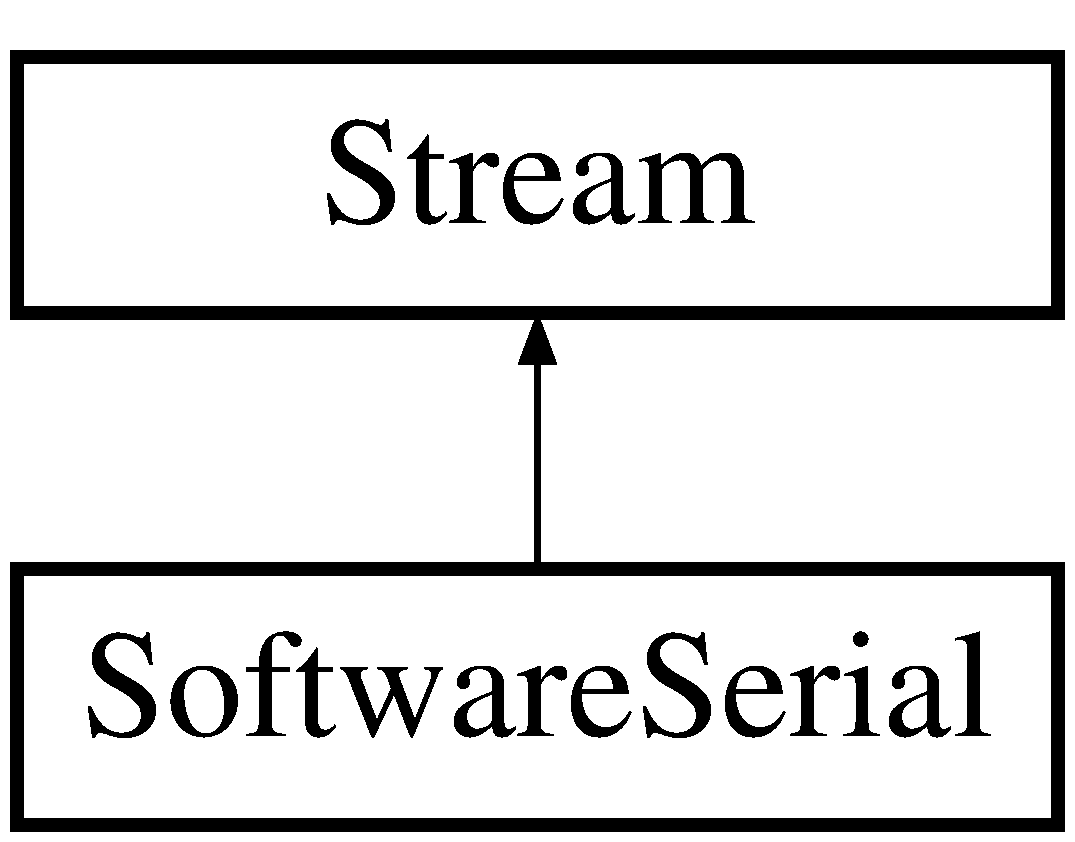
\includegraphics[height=2.000000cm]{class_software_serial}
\end{center}
\end{figure}
\subsection*{Public Member Functions}
\begin{DoxyCompactItemize}
\item 
\hyperlink{class_software_serial_aab36336db4a1ca5073071c07d910cb87}{Software\+Serial} (uint8\+\_\+t receive\+Pin, uint8\+\_\+t transmit\+Pin, bool inverse\+\_\+logic=false)
\item 
\hyperlink{class_software_serial_af6b8fff282e09a6cecc5df669ae71ee7}{$\sim$\+Software\+Serial} ()
\item 
void \hyperlink{class_software_serial_af1b194359d70894b3a2f38236a68480e}{begin} (long speed)
\item 
bool \hyperlink{class_software_serial_ad235539ef28939836bd0bde9387eb8fc}{listen} ()
\item 
void \hyperlink{class_software_serial_a9034270f7de617b3cc7d3f38f3a8e0df}{end} ()
\item 
bool \hyperlink{class_software_serial_a7b3fb4a8f57d2b5f2233f841d71ef80f}{is\+Listening} ()
\item 
bool \hyperlink{class_software_serial_a1c87a6b43c176c104f28e2c2eec2841e}{stop\+Listening} ()
\item 
bool \hyperlink{class_software_serial_ac6d4d5dfbe05515bf23766e2c8abfd46}{overflow} ()
\item 
int \hyperlink{class_software_serial_a51c2d2e79f0d982b1ef9cc9ac4453648}{peek} ()
\item 
virtual size\+\_\+t \hyperlink{class_software_serial_ac24e5c6af203ec636c0a200b0cb3caf0}{write} (uint8\+\_\+t byte)
\item 
virtual int \hyperlink{class_software_serial_a2d0b2f2868d519c716114777f482705b}{read} ()
\item 
virtual int \hyperlink{class_software_serial_a4cbf77a4e90e15ca576972d7952659c5}{available} ()
\item 
virtual void \hyperlink{class_software_serial_a9a46db376a19fc958e011e38799b902c}{flush} ()
\item 
\hyperlink{class_software_serial_ab0cba63b2a27fcfa4760a2f3f7389de0}{operator bool} ()
\end{DoxyCompactItemize}
\subsection*{Static Public Member Functions}
\begin{DoxyCompactItemize}
\item 
static void \hyperlink{class_software_serial_a8700c768d3c5d681362253324852ceee}{handle\+\_\+interrupt} () \+\_\+\+\_\+attribute\+\_\+\+\_\+((\+\_\+\+\_\+always\+\_\+inline\+\_\+\+\_\+))
\end{DoxyCompactItemize}


\subsection{Constructor \& Destructor Documentation}
\hypertarget{class_software_serial_aab36336db4a1ca5073071c07d910cb87}{}\index{Software\+Serial@{Software\+Serial}!Software\+Serial@{Software\+Serial}}
\index{Software\+Serial@{Software\+Serial}!Software\+Serial@{Software\+Serial}}
\subsubsection[{Software\+Serial}]{\setlength{\rightskip}{0pt plus 5cm}Software\+Serial\+::\+Software\+Serial (
\begin{DoxyParamCaption}
\item[{uint8\+\_\+t}]{receive\+Pin, }
\item[{uint8\+\_\+t}]{transmit\+Pin, }
\item[{bool}]{inverse\+\_\+logic = {\ttfamily false}}
\end{DoxyParamCaption}
)}\label{class_software_serial_aab36336db4a1ca5073071c07d910cb87}
\hypertarget{class_software_serial_af6b8fff282e09a6cecc5df669ae71ee7}{}\index{Software\+Serial@{Software\+Serial}!````~Software\+Serial@{$\sim$\+Software\+Serial}}
\index{````~Software\+Serial@{$\sim$\+Software\+Serial}!Software\+Serial@{Software\+Serial}}
\subsubsection[{$\sim$\+Software\+Serial}]{\setlength{\rightskip}{0pt plus 5cm}Software\+Serial\+::$\sim$\+Software\+Serial (
\begin{DoxyParamCaption}
{}
\end{DoxyParamCaption}
)}\label{class_software_serial_af6b8fff282e09a6cecc5df669ae71ee7}


\subsection{Member Function Documentation}
\hypertarget{class_software_serial_a4cbf77a4e90e15ca576972d7952659c5}{}\index{Software\+Serial@{Software\+Serial}!available@{available}}
\index{available@{available}!Software\+Serial@{Software\+Serial}}
\subsubsection[{available}]{\setlength{\rightskip}{0pt plus 5cm}int Software\+Serial\+::available (
\begin{DoxyParamCaption}
\item[{void}]{}
\end{DoxyParamCaption}
)\hspace{0.3cm}{\ttfamily [virtual]}}\label{class_software_serial_a4cbf77a4e90e15ca576972d7952659c5}
\hypertarget{class_software_serial_af1b194359d70894b3a2f38236a68480e}{}\index{Software\+Serial@{Software\+Serial}!begin@{begin}}
\index{begin@{begin}!Software\+Serial@{Software\+Serial}}
\subsubsection[{begin}]{\setlength{\rightskip}{0pt plus 5cm}void Software\+Serial\+::begin (
\begin{DoxyParamCaption}
\item[{long}]{speed}
\end{DoxyParamCaption}
)}\label{class_software_serial_af1b194359d70894b3a2f38236a68480e}
\hypertarget{class_software_serial_a9034270f7de617b3cc7d3f38f3a8e0df}{}\index{Software\+Serial@{Software\+Serial}!end@{end}}
\index{end@{end}!Software\+Serial@{Software\+Serial}}
\subsubsection[{end}]{\setlength{\rightskip}{0pt plus 5cm}void Software\+Serial\+::end (
\begin{DoxyParamCaption}
{}
\end{DoxyParamCaption}
)}\label{class_software_serial_a9034270f7de617b3cc7d3f38f3a8e0df}
\hypertarget{class_software_serial_a9a46db376a19fc958e011e38799b902c}{}\index{Software\+Serial@{Software\+Serial}!flush@{flush}}
\index{flush@{flush}!Software\+Serial@{Software\+Serial}}
\subsubsection[{flush}]{\setlength{\rightskip}{0pt plus 5cm}void Software\+Serial\+::flush (
\begin{DoxyParamCaption}
{}
\end{DoxyParamCaption}
)\hspace{0.3cm}{\ttfamily [virtual]}}\label{class_software_serial_a9a46db376a19fc958e011e38799b902c}
\hypertarget{class_software_serial_a8700c768d3c5d681362253324852ceee}{}\index{Software\+Serial@{Software\+Serial}!handle\+\_\+interrupt@{handle\+\_\+interrupt}}
\index{handle\+\_\+interrupt@{handle\+\_\+interrupt}!Software\+Serial@{Software\+Serial}}
\subsubsection[{handle\+\_\+interrupt}]{\setlength{\rightskip}{0pt plus 5cm}void Software\+Serial\+::handle\+\_\+interrupt (
\begin{DoxyParamCaption}
{}
\end{DoxyParamCaption}
)\hspace{0.3cm}{\ttfamily [inline]}, {\ttfamily [static]}}\label{class_software_serial_a8700c768d3c5d681362253324852ceee}
\hypertarget{class_software_serial_a7b3fb4a8f57d2b5f2233f841d71ef80f}{}\index{Software\+Serial@{Software\+Serial}!is\+Listening@{is\+Listening}}
\index{is\+Listening@{is\+Listening}!Software\+Serial@{Software\+Serial}}
\subsubsection[{is\+Listening}]{\setlength{\rightskip}{0pt plus 5cm}bool Software\+Serial\+::is\+Listening (
\begin{DoxyParamCaption}
{}
\end{DoxyParamCaption}
)\hspace{0.3cm}{\ttfamily [inline]}}\label{class_software_serial_a7b3fb4a8f57d2b5f2233f841d71ef80f}
\hypertarget{class_software_serial_ad235539ef28939836bd0bde9387eb8fc}{}\index{Software\+Serial@{Software\+Serial}!listen@{listen}}
\index{listen@{listen}!Software\+Serial@{Software\+Serial}}
\subsubsection[{listen}]{\setlength{\rightskip}{0pt plus 5cm}bool Software\+Serial\+::listen (
\begin{DoxyParamCaption}
{}
\end{DoxyParamCaption}
)}\label{class_software_serial_ad235539ef28939836bd0bde9387eb8fc}
\hypertarget{class_software_serial_ab0cba63b2a27fcfa4760a2f3f7389de0}{}\index{Software\+Serial@{Software\+Serial}!operator bool@{operator bool}}
\index{operator bool@{operator bool}!Software\+Serial@{Software\+Serial}}
\subsubsection[{operator bool}]{\setlength{\rightskip}{0pt plus 5cm}Software\+Serial\+::operator bool (
\begin{DoxyParamCaption}
{}
\end{DoxyParamCaption}
)\hspace{0.3cm}{\ttfamily [inline]}}\label{class_software_serial_ab0cba63b2a27fcfa4760a2f3f7389de0}
\hypertarget{class_software_serial_ac6d4d5dfbe05515bf23766e2c8abfd46}{}\index{Software\+Serial@{Software\+Serial}!overflow@{overflow}}
\index{overflow@{overflow}!Software\+Serial@{Software\+Serial}}
\subsubsection[{overflow}]{\setlength{\rightskip}{0pt plus 5cm}bool Software\+Serial\+::overflow (
\begin{DoxyParamCaption}
{}
\end{DoxyParamCaption}
)\hspace{0.3cm}{\ttfamily [inline]}}\label{class_software_serial_ac6d4d5dfbe05515bf23766e2c8abfd46}
\hypertarget{class_software_serial_a51c2d2e79f0d982b1ef9cc9ac4453648}{}\index{Software\+Serial@{Software\+Serial}!peek@{peek}}
\index{peek@{peek}!Software\+Serial@{Software\+Serial}}
\subsubsection[{peek}]{\setlength{\rightskip}{0pt plus 5cm}int Software\+Serial\+::peek (
\begin{DoxyParamCaption}
{}
\end{DoxyParamCaption}
)}\label{class_software_serial_a51c2d2e79f0d982b1ef9cc9ac4453648}
\hypertarget{class_software_serial_a2d0b2f2868d519c716114777f482705b}{}\index{Software\+Serial@{Software\+Serial}!read@{read}}
\index{read@{read}!Software\+Serial@{Software\+Serial}}
\subsubsection[{read}]{\setlength{\rightskip}{0pt plus 5cm}int Software\+Serial\+::read (
\begin{DoxyParamCaption}
\item[{void}]{}
\end{DoxyParamCaption}
)\hspace{0.3cm}{\ttfamily [virtual]}}\label{class_software_serial_a2d0b2f2868d519c716114777f482705b}
\hypertarget{class_software_serial_a1c87a6b43c176c104f28e2c2eec2841e}{}\index{Software\+Serial@{Software\+Serial}!stop\+Listening@{stop\+Listening}}
\index{stop\+Listening@{stop\+Listening}!Software\+Serial@{Software\+Serial}}
\subsubsection[{stop\+Listening}]{\setlength{\rightskip}{0pt plus 5cm}bool Software\+Serial\+::stop\+Listening (
\begin{DoxyParamCaption}
{}
\end{DoxyParamCaption}
)}\label{class_software_serial_a1c87a6b43c176c104f28e2c2eec2841e}
\hypertarget{class_software_serial_ac24e5c6af203ec636c0a200b0cb3caf0}{}\index{Software\+Serial@{Software\+Serial}!write@{write}}
\index{write@{write}!Software\+Serial@{Software\+Serial}}
\subsubsection[{write}]{\setlength{\rightskip}{0pt plus 5cm}size\+\_\+t Software\+Serial\+::write (
\begin{DoxyParamCaption}
\item[{uint8\+\_\+t}]{byte}
\end{DoxyParamCaption}
)\hspace{0.3cm}{\ttfamily [virtual]}}\label{class_software_serial_ac24e5c6af203ec636c0a200b0cb3caf0}


The documentation for this class was generated from the following files\+:\begin{DoxyCompactItemize}
\item 
\hyperlink{support__software__serial_8h}{support\+\_\+software\+\_\+serial.\+h}\item 
\hyperlink{support__software__serial_8cpp}{support\+\_\+software\+\_\+serial.\+cpp}\end{DoxyCompactItemize}

\hypertarget{class_two_wire}{}\section{Two\+Wire Class Reference}
\label{class_two_wire}\index{Two\+Wire@{Two\+Wire}}


{\ttfamily \#include $<$support\+\_\+wire.\+h$>$}

Inheritance diagram for Two\+Wire\+:\begin{figure}[H]
\begin{center}
\leavevmode
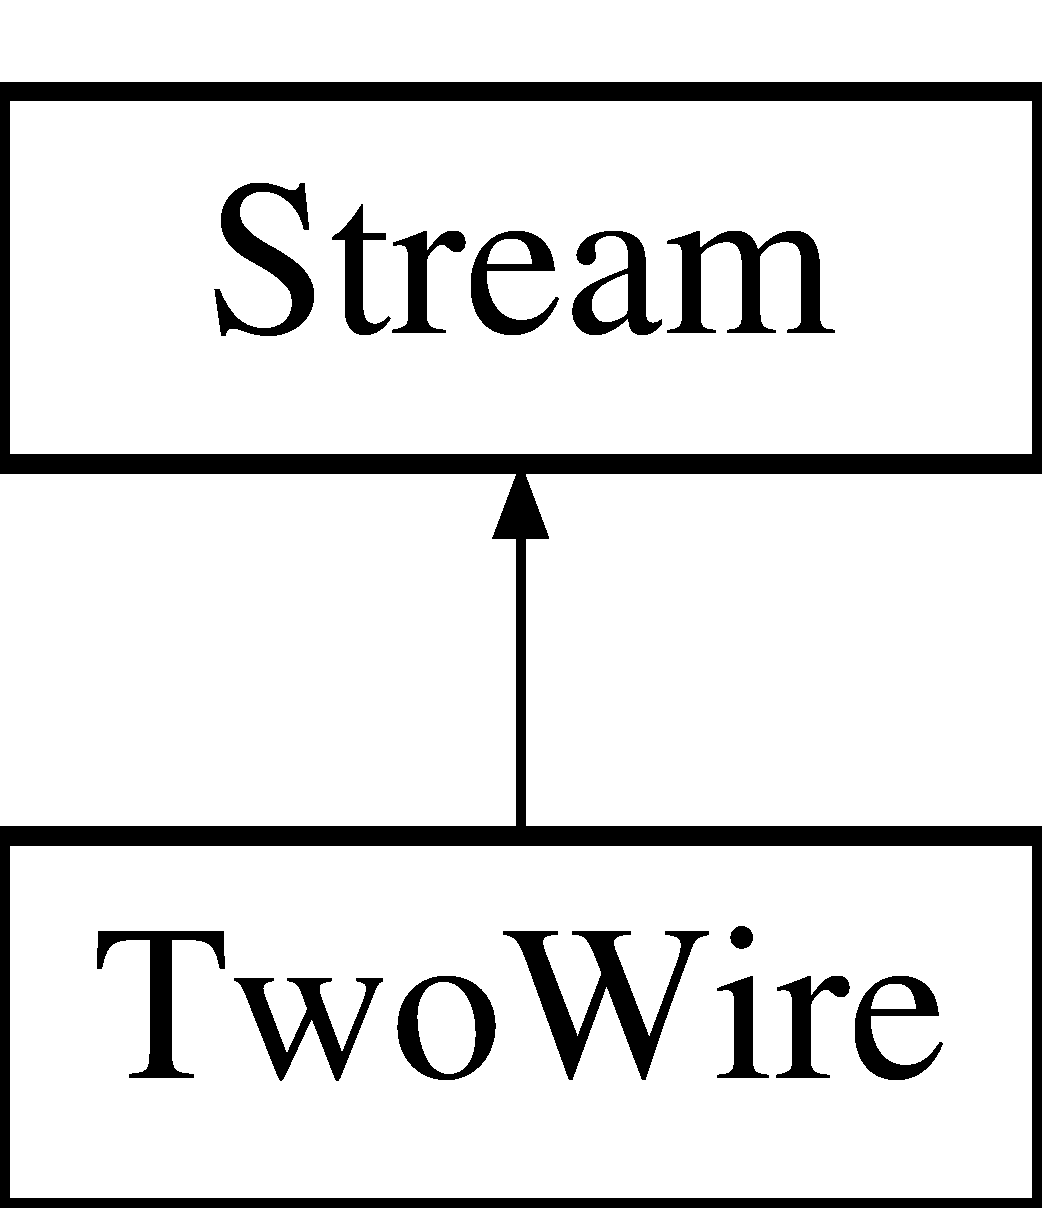
\includegraphics[height=2.000000cm]{class_two_wire}
\end{center}
\end{figure}
\subsection*{Public Member Functions}
\begin{DoxyCompactItemize}
\item 
\hyperlink{class_two_wire_a4c7daf378c06e5e72762e1bd3d5937b6}{Two\+Wire} ()
\item 
void \hyperlink{class_two_wire_ada85a7a8663ec8af0a1248b659be2f18}{begin} ()
\item 
void \hyperlink{class_two_wire_a28bca087ed188781ef15e72622d3b1fb}{begin} (uint8\+\_\+t)
\item 
void \hyperlink{class_two_wire_a2806aa5684d36d7d20bf7c51cab3e602}{begin} (int)
\item 
void \hyperlink{class_two_wire_a3c4aaae8779a8c34d8a1a90ff317d982}{set\+Clock} (uint32\+\_\+t)
\item 
void \hyperlink{class_two_wire_a8d55f00ea8ac3d7427d62e0c71e95ec2}{begin\+Transmission} (uint8\+\_\+t)
\item 
void \hyperlink{class_two_wire_a4da95eb4adced5dad152344243e57aad}{begin\+Transmission} (int)
\item 
uint8\+\_\+t \hyperlink{class_two_wire_af80f9a7b85a3a81a035ca94c95bcdc1d}{end\+Transmission} (void)
\item 
uint8\+\_\+t \hyperlink{class_two_wire_a289f5ef9bb0f79b31095fd72402ed54a}{end\+Transmission} (uint8\+\_\+t)
\item 
uint8\+\_\+t \hyperlink{class_two_wire_ae27d0936487551a05a1e9901bc456599}{request\+From} (uint8\+\_\+t, uint8\+\_\+t)
\item 
uint8\+\_\+t \hyperlink{class_two_wire_a4b4b618531a04d5488a52583a3dfb173}{request\+From} (uint8\+\_\+t, uint8\+\_\+t, uint8\+\_\+t)
\item 
uint8\+\_\+t \hyperlink{class_two_wire_ad40a27213d0bb32f7b819aa8962fccd3}{request\+From} (int, int)
\item 
uint8\+\_\+t \hyperlink{class_two_wire_a3d76da36fb8571e0b5e8310e9f86f6fe}{request\+From} (int, int, int)
\item 
virtual size\+\_\+t \hyperlink{class_two_wire_a318b7bec156c1f1075a818c0ad3427d7}{write} (uint8\+\_\+t)
\item 
virtual size\+\_\+t \hyperlink{class_two_wire_a1957b4d5a6a997bdde436e9e40d131a7}{write} (const uint8\+\_\+t $\ast$, size\+\_\+t)
\item 
virtual int \hyperlink{class_two_wire_aee57bc52bee06508e231c5fc6bc35ada}{available} (void)
\item 
virtual int \hyperlink{class_two_wire_aa361b83500d00dfb93bb25b6473b33e9}{read} (void)
\item 
virtual int \hyperlink{class_two_wire_a5bd64cb7bd609e9470a15d96a0991ec8}{peek} (void)
\item 
virtual void \hyperlink{class_two_wire_a4d92ddf6ca349c815de1de15fca06b5e}{flush} (void)
\item 
void \hyperlink{class_two_wire_a860d97eb825c6fdca388f2f0577cc34a}{on\+Receive} (void($\ast$)(int))
\item 
void \hyperlink{class_two_wire_a224bf8799dda398fc0db223801852ca5}{on\+Request} (void($\ast$)(void))
\item 
size\+\_\+t \hyperlink{class_two_wire_a0c9d09ead8fcddf2a84781fe77d3c975}{write} (unsigned long n)
\item 
size\+\_\+t \hyperlink{class_two_wire_a55a9894186458e43852f6fb7c59bb066}{write} (long n)
\item 
size\+\_\+t \hyperlink{class_two_wire_afdb917746ee37f72e7452b4782e9527b}{write} (unsigned int n)
\item 
size\+\_\+t \hyperlink{class_two_wire_a8ec34b0d2a75e8b2751eb9f4332bd7c3}{write} (int n)
\end{DoxyCompactItemize}


\subsection{Constructor \& Destructor Documentation}
\hypertarget{class_two_wire_a4c7daf378c06e5e72762e1bd3d5937b6}{}\index{Two\+Wire@{Two\+Wire}!Two\+Wire@{Two\+Wire}}
\index{Two\+Wire@{Two\+Wire}!Two\+Wire@{Two\+Wire}}
\subsubsection[{Two\+Wire}]{\setlength{\rightskip}{0pt plus 5cm}Two\+Wire\+::\+Two\+Wire (
\begin{DoxyParamCaption}
{}
\end{DoxyParamCaption}
)}\label{class_two_wire_a4c7daf378c06e5e72762e1bd3d5937b6}


\subsection{Member Function Documentation}
\hypertarget{class_two_wire_aee57bc52bee06508e231c5fc6bc35ada}{}\index{Two\+Wire@{Two\+Wire}!available@{available}}
\index{available@{available}!Two\+Wire@{Two\+Wire}}
\subsubsection[{available}]{\setlength{\rightskip}{0pt plus 5cm}int Two\+Wire\+::available (
\begin{DoxyParamCaption}
\item[{void}]{}
\end{DoxyParamCaption}
)\hspace{0.3cm}{\ttfamily [virtual]}}\label{class_two_wire_aee57bc52bee06508e231c5fc6bc35ada}
\hypertarget{class_two_wire_ada85a7a8663ec8af0a1248b659be2f18}{}\index{Two\+Wire@{Two\+Wire}!begin@{begin}}
\index{begin@{begin}!Two\+Wire@{Two\+Wire}}
\subsubsection[{begin}]{\setlength{\rightskip}{0pt plus 5cm}void Two\+Wire\+::begin (
\begin{DoxyParamCaption}
\item[{void}]{}
\end{DoxyParamCaption}
)}\label{class_two_wire_ada85a7a8663ec8af0a1248b659be2f18}
\hypertarget{class_two_wire_a28bca087ed188781ef15e72622d3b1fb}{}\index{Two\+Wire@{Two\+Wire}!begin@{begin}}
\index{begin@{begin}!Two\+Wire@{Two\+Wire}}
\subsubsection[{begin}]{\setlength{\rightskip}{0pt plus 5cm}void Two\+Wire\+::begin (
\begin{DoxyParamCaption}
\item[{uint8\+\_\+t}]{address}
\end{DoxyParamCaption}
)}\label{class_two_wire_a28bca087ed188781ef15e72622d3b1fb}
\hypertarget{class_two_wire_a2806aa5684d36d7d20bf7c51cab3e602}{}\index{Two\+Wire@{Two\+Wire}!begin@{begin}}
\index{begin@{begin}!Two\+Wire@{Two\+Wire}}
\subsubsection[{begin}]{\setlength{\rightskip}{0pt plus 5cm}void Two\+Wire\+::begin (
\begin{DoxyParamCaption}
\item[{int}]{address}
\end{DoxyParamCaption}
)}\label{class_two_wire_a2806aa5684d36d7d20bf7c51cab3e602}
\hypertarget{class_two_wire_a8d55f00ea8ac3d7427d62e0c71e95ec2}{}\index{Two\+Wire@{Two\+Wire}!begin\+Transmission@{begin\+Transmission}}
\index{begin\+Transmission@{begin\+Transmission}!Two\+Wire@{Two\+Wire}}
\subsubsection[{begin\+Transmission}]{\setlength{\rightskip}{0pt plus 5cm}void Two\+Wire\+::begin\+Transmission (
\begin{DoxyParamCaption}
\item[{uint8\+\_\+t}]{address}
\end{DoxyParamCaption}
)}\label{class_two_wire_a8d55f00ea8ac3d7427d62e0c71e95ec2}
\hypertarget{class_two_wire_a4da95eb4adced5dad152344243e57aad}{}\index{Two\+Wire@{Two\+Wire}!begin\+Transmission@{begin\+Transmission}}
\index{begin\+Transmission@{begin\+Transmission}!Two\+Wire@{Two\+Wire}}
\subsubsection[{begin\+Transmission}]{\setlength{\rightskip}{0pt plus 5cm}void Two\+Wire\+::begin\+Transmission (
\begin{DoxyParamCaption}
\item[{int}]{address}
\end{DoxyParamCaption}
)}\label{class_two_wire_a4da95eb4adced5dad152344243e57aad}
\hypertarget{class_two_wire_af80f9a7b85a3a81a035ca94c95bcdc1d}{}\index{Two\+Wire@{Two\+Wire}!end\+Transmission@{end\+Transmission}}
\index{end\+Transmission@{end\+Transmission}!Two\+Wire@{Two\+Wire}}
\subsubsection[{end\+Transmission}]{\setlength{\rightskip}{0pt plus 5cm}uint8\+\_\+t Two\+Wire\+::end\+Transmission (
\begin{DoxyParamCaption}
\item[{void}]{}
\end{DoxyParamCaption}
)}\label{class_two_wire_af80f9a7b85a3a81a035ca94c95bcdc1d}
\hypertarget{class_two_wire_a289f5ef9bb0f79b31095fd72402ed54a}{}\index{Two\+Wire@{Two\+Wire}!end\+Transmission@{end\+Transmission}}
\index{end\+Transmission@{end\+Transmission}!Two\+Wire@{Two\+Wire}}
\subsubsection[{end\+Transmission}]{\setlength{\rightskip}{0pt plus 5cm}uint8\+\_\+t Two\+Wire\+::end\+Transmission (
\begin{DoxyParamCaption}
\item[{uint8\+\_\+t}]{send\+Stop}
\end{DoxyParamCaption}
)}\label{class_two_wire_a289f5ef9bb0f79b31095fd72402ed54a}
\hypertarget{class_two_wire_a4d92ddf6ca349c815de1de15fca06b5e}{}\index{Two\+Wire@{Two\+Wire}!flush@{flush}}
\index{flush@{flush}!Two\+Wire@{Two\+Wire}}
\subsubsection[{flush}]{\setlength{\rightskip}{0pt plus 5cm}void Two\+Wire\+::flush (
\begin{DoxyParamCaption}
\item[{void}]{}
\end{DoxyParamCaption}
)\hspace{0.3cm}{\ttfamily [virtual]}}\label{class_two_wire_a4d92ddf6ca349c815de1de15fca06b5e}
\hypertarget{class_two_wire_a860d97eb825c6fdca388f2f0577cc34a}{}\index{Two\+Wire@{Two\+Wire}!on\+Receive@{on\+Receive}}
\index{on\+Receive@{on\+Receive}!Two\+Wire@{Two\+Wire}}
\subsubsection[{on\+Receive}]{\setlength{\rightskip}{0pt plus 5cm}void Two\+Wire\+::on\+Receive (
\begin{DoxyParamCaption}
\item[{void($\ast$)(int)}]{function}
\end{DoxyParamCaption}
)}\label{class_two_wire_a860d97eb825c6fdca388f2f0577cc34a}
\hypertarget{class_two_wire_a224bf8799dda398fc0db223801852ca5}{}\index{Two\+Wire@{Two\+Wire}!on\+Request@{on\+Request}}
\index{on\+Request@{on\+Request}!Two\+Wire@{Two\+Wire}}
\subsubsection[{on\+Request}]{\setlength{\rightskip}{0pt plus 5cm}void Two\+Wire\+::on\+Request (
\begin{DoxyParamCaption}
\item[{void($\ast$)(void)}]{function}
\end{DoxyParamCaption}
)}\label{class_two_wire_a224bf8799dda398fc0db223801852ca5}
\hypertarget{class_two_wire_a5bd64cb7bd609e9470a15d96a0991ec8}{}\index{Two\+Wire@{Two\+Wire}!peek@{peek}}
\index{peek@{peek}!Two\+Wire@{Two\+Wire}}
\subsubsection[{peek}]{\setlength{\rightskip}{0pt plus 5cm}int Two\+Wire\+::peek (
\begin{DoxyParamCaption}
\item[{void}]{}
\end{DoxyParamCaption}
)\hspace{0.3cm}{\ttfamily [virtual]}}\label{class_two_wire_a5bd64cb7bd609e9470a15d96a0991ec8}
\hypertarget{class_two_wire_aa361b83500d00dfb93bb25b6473b33e9}{}\index{Two\+Wire@{Two\+Wire}!read@{read}}
\index{read@{read}!Two\+Wire@{Two\+Wire}}
\subsubsection[{read}]{\setlength{\rightskip}{0pt plus 5cm}int Two\+Wire\+::read (
\begin{DoxyParamCaption}
\item[{void}]{}
\end{DoxyParamCaption}
)\hspace{0.3cm}{\ttfamily [virtual]}}\label{class_two_wire_aa361b83500d00dfb93bb25b6473b33e9}
\hypertarget{class_two_wire_ae27d0936487551a05a1e9901bc456599}{}\index{Two\+Wire@{Two\+Wire}!request\+From@{request\+From}}
\index{request\+From@{request\+From}!Two\+Wire@{Two\+Wire}}
\subsubsection[{request\+From}]{\setlength{\rightskip}{0pt plus 5cm}uint8\+\_\+t Two\+Wire\+::request\+From (
\begin{DoxyParamCaption}
\item[{uint8\+\_\+t}]{address, }
\item[{uint8\+\_\+t}]{quantity}
\end{DoxyParamCaption}
)}\label{class_two_wire_ae27d0936487551a05a1e9901bc456599}
\hypertarget{class_two_wire_a4b4b618531a04d5488a52583a3dfb173}{}\index{Two\+Wire@{Two\+Wire}!request\+From@{request\+From}}
\index{request\+From@{request\+From}!Two\+Wire@{Two\+Wire}}
\subsubsection[{request\+From}]{\setlength{\rightskip}{0pt plus 5cm}uint8\+\_\+t Two\+Wire\+::request\+From (
\begin{DoxyParamCaption}
\item[{uint8\+\_\+t}]{address, }
\item[{uint8\+\_\+t}]{quantity, }
\item[{uint8\+\_\+t}]{send\+Stop}
\end{DoxyParamCaption}
)}\label{class_two_wire_a4b4b618531a04d5488a52583a3dfb173}
\hypertarget{class_two_wire_ad40a27213d0bb32f7b819aa8962fccd3}{}\index{Two\+Wire@{Two\+Wire}!request\+From@{request\+From}}
\index{request\+From@{request\+From}!Two\+Wire@{Two\+Wire}}
\subsubsection[{request\+From}]{\setlength{\rightskip}{0pt plus 5cm}uint8\+\_\+t Two\+Wire\+::request\+From (
\begin{DoxyParamCaption}
\item[{int}]{address, }
\item[{int}]{quantity}
\end{DoxyParamCaption}
)}\label{class_two_wire_ad40a27213d0bb32f7b819aa8962fccd3}
\hypertarget{class_two_wire_a3d76da36fb8571e0b5e8310e9f86f6fe}{}\index{Two\+Wire@{Two\+Wire}!request\+From@{request\+From}}
\index{request\+From@{request\+From}!Two\+Wire@{Two\+Wire}}
\subsubsection[{request\+From}]{\setlength{\rightskip}{0pt plus 5cm}uint8\+\_\+t Two\+Wire\+::request\+From (
\begin{DoxyParamCaption}
\item[{int}]{address, }
\item[{int}]{quantity, }
\item[{int}]{send\+Stop}
\end{DoxyParamCaption}
)}\label{class_two_wire_a3d76da36fb8571e0b5e8310e9f86f6fe}
\hypertarget{class_two_wire_a3c4aaae8779a8c34d8a1a90ff317d982}{}\index{Two\+Wire@{Two\+Wire}!set\+Clock@{set\+Clock}}
\index{set\+Clock@{set\+Clock}!Two\+Wire@{Two\+Wire}}
\subsubsection[{set\+Clock}]{\setlength{\rightskip}{0pt plus 5cm}void Two\+Wire\+::set\+Clock (
\begin{DoxyParamCaption}
\item[{uint32\+\_\+t}]{frequency}
\end{DoxyParamCaption}
)}\label{class_two_wire_a3c4aaae8779a8c34d8a1a90ff317d982}
\hypertarget{class_two_wire_a318b7bec156c1f1075a818c0ad3427d7}{}\index{Two\+Wire@{Two\+Wire}!write@{write}}
\index{write@{write}!Two\+Wire@{Two\+Wire}}
\subsubsection[{write}]{\setlength{\rightskip}{0pt plus 5cm}size\+\_\+t Two\+Wire\+::write (
\begin{DoxyParamCaption}
\item[{uint8\+\_\+t}]{data}
\end{DoxyParamCaption}
)\hspace{0.3cm}{\ttfamily [virtual]}}\label{class_two_wire_a318b7bec156c1f1075a818c0ad3427d7}
\hypertarget{class_two_wire_a1957b4d5a6a997bdde436e9e40d131a7}{}\index{Two\+Wire@{Two\+Wire}!write@{write}}
\index{write@{write}!Two\+Wire@{Two\+Wire}}
\subsubsection[{write}]{\setlength{\rightskip}{0pt plus 5cm}size\+\_\+t Two\+Wire\+::write (
\begin{DoxyParamCaption}
\item[{const uint8\+\_\+t $\ast$}]{data, }
\item[{size\+\_\+t}]{quantity}
\end{DoxyParamCaption}
)\hspace{0.3cm}{\ttfamily [virtual]}}\label{class_two_wire_a1957b4d5a6a997bdde436e9e40d131a7}
\hypertarget{class_two_wire_a0c9d09ead8fcddf2a84781fe77d3c975}{}\index{Two\+Wire@{Two\+Wire}!write@{write}}
\index{write@{write}!Two\+Wire@{Two\+Wire}}
\subsubsection[{write}]{\setlength{\rightskip}{0pt plus 5cm}size\+\_\+t Two\+Wire\+::write (
\begin{DoxyParamCaption}
\item[{unsigned long}]{n}
\end{DoxyParamCaption}
)\hspace{0.3cm}{\ttfamily [inline]}}\label{class_two_wire_a0c9d09ead8fcddf2a84781fe77d3c975}
\hypertarget{class_two_wire_a55a9894186458e43852f6fb7c59bb066}{}\index{Two\+Wire@{Two\+Wire}!write@{write}}
\index{write@{write}!Two\+Wire@{Two\+Wire}}
\subsubsection[{write}]{\setlength{\rightskip}{0pt plus 5cm}size\+\_\+t Two\+Wire\+::write (
\begin{DoxyParamCaption}
\item[{long}]{n}
\end{DoxyParamCaption}
)\hspace{0.3cm}{\ttfamily [inline]}}\label{class_two_wire_a55a9894186458e43852f6fb7c59bb066}
\hypertarget{class_two_wire_afdb917746ee37f72e7452b4782e9527b}{}\index{Two\+Wire@{Two\+Wire}!write@{write}}
\index{write@{write}!Two\+Wire@{Two\+Wire}}
\subsubsection[{write}]{\setlength{\rightskip}{0pt plus 5cm}size\+\_\+t Two\+Wire\+::write (
\begin{DoxyParamCaption}
\item[{unsigned int}]{n}
\end{DoxyParamCaption}
)\hspace{0.3cm}{\ttfamily [inline]}}\label{class_two_wire_afdb917746ee37f72e7452b4782e9527b}
\hypertarget{class_two_wire_a8ec34b0d2a75e8b2751eb9f4332bd7c3}{}\index{Two\+Wire@{Two\+Wire}!write@{write}}
\index{write@{write}!Two\+Wire@{Two\+Wire}}
\subsubsection[{write}]{\setlength{\rightskip}{0pt plus 5cm}size\+\_\+t Two\+Wire\+::write (
\begin{DoxyParamCaption}
\item[{int}]{n}
\end{DoxyParamCaption}
)\hspace{0.3cm}{\ttfamily [inline]}}\label{class_two_wire_a8ec34b0d2a75e8b2751eb9f4332bd7c3}


The documentation for this class was generated from the following files\+:\begin{DoxyCompactItemize}
\item 
\hyperlink{support__wire_8h}{support\+\_\+wire.\+h}\item 
\hyperlink{support__wire_8cpp}{support\+\_\+wire.\+cpp}\end{DoxyCompactItemize}

\chapter{File Documentation}
\hypertarget{actuator__relay_8cpp}{}\section{actuator\+\_\+relay.\+cpp File Reference}
\label{actuator__relay_8cpp}\index{actuator\+\_\+relay.\+cpp@{actuator\+\_\+relay.\+cpp}}
{\ttfamily \#include \char`\"{}actuator\+\_\+relay.\+h\char`\"{}}\\*

\hypertarget{actuator__relay_8h}{}\section{actuator\+\_\+relay.\+h File Reference}
\label{actuator__relay_8h}\index{actuator\+\_\+relay.\+h@{actuator\+\_\+relay.\+h}}


Actuator module for an active low relay.  


{\ttfamily \#include \char`\"{}W\+Program.\+h\char`\"{}}\\*
\subsection*{Classes}
\begin{DoxyCompactItemize}
\item 
class \hyperlink{class_actuator_relay}{Actuator\+Relay}
\end{DoxyCompactItemize}


\subsection{Detailed Description}
Actuator module for an active low relay. 

\begin{DoxyAuthor}{Author}
Jake Rye 
\end{DoxyAuthor}

\hypertarget{communication_8cpp}{}\section{communication.\+cpp File Reference}
\label{communication_8cpp}\index{communication.\+cpp@{communication.\+cpp}}
{\ttfamily \#include \char`\"{}communication.\+h\char`\"{}}\\*

\hypertarget{communication_8h}{}\section{communication.\+h File Reference}
\label{communication_8h}\index{communication.\+h@{communication.\+h}}
{\ttfamily \#include \char`\"{}W\+Program.\+h\char`\"{}}\\*
\subsection*{Classes}
\begin{DoxyCompactItemize}
\item 
class \hyperlink{class_communication}{Communication}
\end{DoxyCompactItemize}

\hypertarget{groduino_8ino}{}\section{groduino.\+ino File Reference}
\label{groduino_8ino}\index{groduino.\+ino@{groduino.\+ino}}

\hypertarget{module__handler_8cpp}{}\section{module\+\_\+handler.\+cpp File Reference}
\label{module__handler_8cpp}\index{module\+\_\+handler.\+cpp@{module\+\_\+handler.\+cpp}}


Handles all module integration. See \hyperlink{module__handler_8h}{module\+\_\+handler.\+h} for details.  


{\ttfamily \#include \char`\"{}module\+\_\+handler.\+h\char`\"{}}\\*
{\ttfamily \#include \char`\"{}communication.\+h\char`\"{}}\\*
{\ttfamily \#include \char`\"{}sensor\+\_\+tsl2561.\+h\char`\"{}}\\*
{\ttfamily \#include \char`\"{}sensor\+\_\+dht22.\+h\char`\"{}}\\*
{\ttfamily \#include \char`\"{}sensor\+\_\+gc0011.\+h\char`\"{}}\\*
{\ttfamily \#include \char`\"{}sensor\+\_\+dfr0161.\+h\char`\"{}}\\*
{\ttfamily \#include \char`\"{}actuator\+\_\+relay.\+h\char`\"{}}\\*
{\ttfamily \#include \char`\"{}sensor\+\_\+dfr0300.\+h\char`\"{}}\\*
{\ttfamily \#include \char`\"{}sensor\+\_\+contact\+\_\+switch.\+h\char`\"{}}\\*
\subsection*{Functions}
\begin{DoxyCompactItemize}
\item 
void \hyperlink{module__handler_8cpp_a691a0d8c2404cb4ce0c088e9857560ee}{update\+Incoming\+Message} (void)
\begin{DoxyCompactList}\small\item\em Handles all incoming messages from the controller. If new message is available, receive message and pass to handler function. If handler function returns response message, send out. \end{DoxyCompactList}\item 
\hyperlink{struct_instruction}{Instruction} \hyperlink{module__handler_8cpp_afcbd04d77356acd5e3dcf91fefb8bd11}{parse\+Incoming\+Message} (String message)
\begin{DoxyCompactList}\small\item\em Formats an instruction string into an instruction struct. Message is broken into 3 parts\+: \hyperlink{struct_instruction}{Instruction} Code, \hyperlink{struct_instruction}{Instruction} I\+D, \hyperlink{struct_instruction}{Instruction} Parameter then returns the parts as an \hyperlink{struct_instruction}{Instruction} Object Also, the \hyperlink{struct_instruction}{Instruction} Valid parameter is set accordingly. \end{DoxyCompactList}\item 
void \hyperlink{module__handler_8cpp_aea7eb84b3bdf67ce76b8b3d1a7c1b64d}{initialize\+Modules} (void)
\begin{DoxyCompactList}\small\item\em Called once to initialize all modules. Runs once at the beginning of the program. Calls all module $\ast$.begin() functions. \end{DoxyCompactList}\item 
void \hyperlink{module__handler_8cpp_a5897de55f349106cd3e341df9bc6ddcd}{update\+Stream\+Message} (void)
\begin{DoxyCompactList}\small\item\em Handles all outgoing messages to the controller. Polls all objects using their $\ast$.get() function and appends to message stream Sends message stream to controller. \end{DoxyCompactList}\item 
String \hyperlink{module__handler_8cpp_a84d5c9e2f57b3fcb377800f72edea419}{handle\+Incoming\+Message} (void)
\begin{DoxyCompactList}\small\item\em Messages from controller are handled by this function. Each message is a single instruction string. \hyperlink{struct_instruction}{Instruction} string gets broken into instruction code, id, and parameter. Passed in piecewise to $<$module$>$.set function. If a return message is generated from the $<$module$>$.set function, this function returns that message. \end{DoxyCompactList}\end{DoxyCompactItemize}
\subsection*{Variables}
\begin{DoxyCompactItemize}
\item 
\hyperlink{class_communication}{Communication} \hyperlink{module__handler_8cpp_ae162b537f743c1fa3e4b3a398324649d}{communication} (0)
\item 
\hyperlink{class_sensor_tsl2561}{Sensor\+Tsl2561} \hyperlink{module__handler_8cpp_ac80bfd1cbb89a121918c276b790b790e}{sensor\+\_\+tsl2561\+\_\+light\+\_\+intensity\+\_\+default} (\char`\"{}S\+L\+I\+N\char`\"{}, 1,\char`\"{}S\+L\+P\+A\char`\"{}, 1)
\item 
\hyperlink{class_sensor_dht22}{Sensor\+Dht22} \hyperlink{module__handler_8cpp_a71b8e34ff72f1d153e53311443c419e6}{sensor\+\_\+dht22\+\_\+air\+\_\+temperature\+\_\+humidity\+\_\+default} (A0,\char`\"{}S\+A\+T\+M\char`\"{}, 1,\char`\"{}S\+A\+H\+U\char`\"{}, 1)
\item 
\hyperlink{class_sensor_gc0011}{Sensor\+Gc0011} \hyperlink{module__handler_8cpp_a8875593f7e7ffa5750599fe64d0cb659}{sensor\+\_\+gc0011\+\_\+air\+\_\+co2\+\_\+temperature\+\_\+humidity\+\_\+default} (12, 11,\char`\"{}S\+A\+C\+O\char`\"{}, 1,\char`\"{}S\+A\+T\+M\char`\"{}, 2,\char`\"{}S\+A\+H\+U\char`\"{}, 2)
\item 
\hyperlink{class_sensor_dfr0161}{Sensor\+Dfr0161} \hyperlink{module__handler_8cpp_a1ca73f6d0c3361a7fc59d0b07ab1750d}{sensor\+\_\+dfr0161\+\_\+water\+\_\+ph\+\_\+default} (A1,\char`\"{}S\+W\+P\+H\char`\"{}, 1)
\item 
\hyperlink{class_sensor_dfr0300}{Sensor\+Dfr0300} \hyperlink{module__handler_8cpp_a88260dc0f33287b1462b533e4dc127b2}{sensor\+\_\+dfr0300\+\_\+water\+\_\+temperature\+\_\+ec\+\_\+default} (5, A2, 2,\char`\"{}S\+W\+T\+M\char`\"{}, 1,\char`\"{}S\+W\+E\+C\char`\"{}, 1)
\item 
\hyperlink{class_sensor_contact_switch}{Sensor\+Contact\+Switch} \hyperlink{module__handler_8cpp_aa9f3da0083131fdbd8cf03f27cf9d551}{sensor\+\_\+contact\+\_\+switch\+\_\+general\+\_\+shell\+\_\+open\+\_\+default} (4,\char`\"{}S\+G\+S\+O\char`\"{}, 1)
\item 
\hyperlink{class_sensor_contact_switch}{Sensor\+Contact\+Switch} \hyperlink{module__handler_8cpp_ab6630028881a21e75bbe48305c5604f7}{sensor\+\_\+contact\+\_\+switch\+\_\+general\+\_\+window\+\_\+open\+\_\+default} (3,\char`\"{}S\+G\+W\+O\char`\"{}, 1)
\item 
\hyperlink{class_actuator_relay}{Actuator\+Relay} \hyperlink{module__handler_8cpp_a0a937c87b9401ed7584696b6923185f3}{actuator\+\_\+relay\+\_\+air\+\_\+heater\+\_\+default} (6,\char`\"{}A\+A\+H\+E\char`\"{}, 1)
\item 
\hyperlink{class_actuator_relay}{Actuator\+Relay} \hyperlink{module__handler_8cpp_a8332988d91deeba745badf4ca8ad163e}{actuator\+\_\+relay\+\_\+light\+\_\+panel\+\_\+default} (8,\char`\"{}A\+L\+P\+N\char`\"{}, 1)
\item 
\hyperlink{class_actuator_relay}{Actuator\+Relay} \hyperlink{module__handler_8cpp_a0e86deb38503c2cf91314642c78cdfd3}{actuator\+\_\+relay\+\_\+air\+\_\+humidifier\+\_\+default} (9,\char`\"{}A\+A\+H\+U\char`\"{}, 1)
\item 
\hyperlink{class_actuator_relay}{Actuator\+Relay} \hyperlink{module__handler_8cpp_a25c0b2af14a6fb79b2f25ec1df8c838e}{actuator\+\_\+relay\+\_\+air\+\_\+vent\+\_\+default} (14,\char`\"{}A\+A\+V\+E\char`\"{}, 1)
\item 
\hyperlink{class_actuator_relay}{Actuator\+Relay} \hyperlink{module__handler_8cpp_a3f0b6a49faffb54d8af560b9dc3b4cc0}{actuator\+\_\+relay\+\_\+air\+\_\+circulation\+\_\+default} (15,\char`\"{}A\+A\+C\+R\char`\"{}, 1)
\item 
\hyperlink{class_actuator_relay}{Actuator\+Relay} \hyperlink{module__handler_8cpp_a804b6a7c6d635c11d5dd634e016e7f3b}{actuator\+\_\+relay\+\_\+light\+\_\+chamber\+\_\+illumination\+\_\+default} (53,\char`\"{}A\+L\+P\+N\char`\"{}, 2)
\item 
\hyperlink{class_actuator_relay}{Actuator\+Relay} \hyperlink{module__handler_8cpp_a10f9d41c1003f37e9036eb87416e30c2}{actuator\+\_\+relay\+\_\+light\+\_\+motherboard\+\_\+illumination\+\_\+default} (52,\char`\"{}A\+L\+M\+I\char`\"{}, 1)
\end{DoxyCompactItemize}


\subsection{Detailed Description}
Handles all module integration. See \hyperlink{module__handler_8h}{module\+\_\+handler.\+h} for details. 

\begin{DoxyAuthor}{Author}
Jake Rye 
\end{DoxyAuthor}


\subsection{Function Documentation}
\hypertarget{module__handler_8cpp_a84d5c9e2f57b3fcb377800f72edea419}{}\index{module\+\_\+handler.\+cpp@{module\+\_\+handler.\+cpp}!handle\+Incoming\+Message@{handle\+Incoming\+Message}}
\index{handle\+Incoming\+Message@{handle\+Incoming\+Message}!module\+\_\+handler.\+cpp@{module\+\_\+handler.\+cpp}}
\subsubsection[{handle\+Incoming\+Message}]{\setlength{\rightskip}{0pt plus 5cm}String handle\+Incoming\+Message (
\begin{DoxyParamCaption}
\item[{void}]{}
\end{DoxyParamCaption}
)}\label{module__handler_8cpp_a84d5c9e2f57b3fcb377800f72edea419}


Messages from controller are handled by this function. Each message is a single instruction string. \hyperlink{struct_instruction}{Instruction} string gets broken into instruction code, id, and parameter. Passed in piecewise to $<$module$>$.set function. If a return message is generated from the $<$module$>$.set function, this function returns that message. 

\hypertarget{module__handler_8cpp_aea7eb84b3bdf67ce76b8b3d1a7c1b64d}{}\index{module\+\_\+handler.\+cpp@{module\+\_\+handler.\+cpp}!initialize\+Modules@{initialize\+Modules}}
\index{initialize\+Modules@{initialize\+Modules}!module\+\_\+handler.\+cpp@{module\+\_\+handler.\+cpp}}
\subsubsection[{initialize\+Modules}]{\setlength{\rightskip}{0pt plus 5cm}void initialize\+Modules (
\begin{DoxyParamCaption}
\item[{void}]{}
\end{DoxyParamCaption}
)}\label{module__handler_8cpp_aea7eb84b3bdf67ce76b8b3d1a7c1b64d}


Called once to initialize all modules. Runs once at the beginning of the program. Calls all module $\ast$.begin() functions. 

\hypertarget{module__handler_8cpp_afcbd04d77356acd5e3dcf91fefb8bd11}{}\index{module\+\_\+handler.\+cpp@{module\+\_\+handler.\+cpp}!parse\+Incoming\+Message@{parse\+Incoming\+Message}}
\index{parse\+Incoming\+Message@{parse\+Incoming\+Message}!module\+\_\+handler.\+cpp@{module\+\_\+handler.\+cpp}}
\subsubsection[{parse\+Incoming\+Message}]{\setlength{\rightskip}{0pt plus 5cm}{\bf Instruction} parse\+Incoming\+Message (
\begin{DoxyParamCaption}
\item[{String}]{message}
\end{DoxyParamCaption}
)}\label{module__handler_8cpp_afcbd04d77356acd5e3dcf91fefb8bd11}


Formats an instruction string into an instruction struct. Message is broken into 3 parts\+: \hyperlink{struct_instruction}{Instruction} Code, \hyperlink{struct_instruction}{Instruction} I\+D, \hyperlink{struct_instruction}{Instruction} Parameter then returns the parts as an \hyperlink{struct_instruction}{Instruction} Object Also, the \hyperlink{struct_instruction}{Instruction} Valid parameter is set accordingly. 

\hypertarget{module__handler_8cpp_a691a0d8c2404cb4ce0c088e9857560ee}{}\index{module\+\_\+handler.\+cpp@{module\+\_\+handler.\+cpp}!update\+Incoming\+Message@{update\+Incoming\+Message}}
\index{update\+Incoming\+Message@{update\+Incoming\+Message}!module\+\_\+handler.\+cpp@{module\+\_\+handler.\+cpp}}
\subsubsection[{update\+Incoming\+Message}]{\setlength{\rightskip}{0pt plus 5cm}void update\+Incoming\+Message (
\begin{DoxyParamCaption}
\item[{void}]{}
\end{DoxyParamCaption}
)}\label{module__handler_8cpp_a691a0d8c2404cb4ce0c088e9857560ee}


Handles all incoming messages from the controller. If new message is available, receive message and pass to handler function. If handler function returns response message, send out. 

\hypertarget{module__handler_8cpp_a5897de55f349106cd3e341df9bc6ddcd}{}\index{module\+\_\+handler.\+cpp@{module\+\_\+handler.\+cpp}!update\+Stream\+Message@{update\+Stream\+Message}}
\index{update\+Stream\+Message@{update\+Stream\+Message}!module\+\_\+handler.\+cpp@{module\+\_\+handler.\+cpp}}
\subsubsection[{update\+Stream\+Message}]{\setlength{\rightskip}{0pt plus 5cm}void update\+Stream\+Message (
\begin{DoxyParamCaption}
\item[{void}]{}
\end{DoxyParamCaption}
)}\label{module__handler_8cpp_a5897de55f349106cd3e341df9bc6ddcd}


Handles all outgoing messages to the controller. Polls all objects using their $\ast$.get() function and appends to message stream Sends message stream to controller. 



\subsection{Variable Documentation}
\hypertarget{module__handler_8cpp_a3f0b6a49faffb54d8af560b9dc3b4cc0}{}\index{module\+\_\+handler.\+cpp@{module\+\_\+handler.\+cpp}!actuator\+\_\+relay\+\_\+air\+\_\+circulation\+\_\+default@{actuator\+\_\+relay\+\_\+air\+\_\+circulation\+\_\+default}}
\index{actuator\+\_\+relay\+\_\+air\+\_\+circulation\+\_\+default@{actuator\+\_\+relay\+\_\+air\+\_\+circulation\+\_\+default}!module\+\_\+handler.\+cpp@{module\+\_\+handler.\+cpp}}
\subsubsection[{actuator\+\_\+relay\+\_\+air\+\_\+circulation\+\_\+default}]{\setlength{\rightskip}{0pt plus 5cm}{\bf Actuator\+Relay} actuator\+\_\+relay\+\_\+air\+\_\+circulation\+\_\+default(15,\char`\"{}A\+A\+C\+R\char`\"{}, 1)}\label{module__handler_8cpp_a3f0b6a49faffb54d8af560b9dc3b4cc0}
\hypertarget{module__handler_8cpp_a0a937c87b9401ed7584696b6923185f3}{}\index{module\+\_\+handler.\+cpp@{module\+\_\+handler.\+cpp}!actuator\+\_\+relay\+\_\+air\+\_\+heater\+\_\+default@{actuator\+\_\+relay\+\_\+air\+\_\+heater\+\_\+default}}
\index{actuator\+\_\+relay\+\_\+air\+\_\+heater\+\_\+default@{actuator\+\_\+relay\+\_\+air\+\_\+heater\+\_\+default}!module\+\_\+handler.\+cpp@{module\+\_\+handler.\+cpp}}
\subsubsection[{actuator\+\_\+relay\+\_\+air\+\_\+heater\+\_\+default}]{\setlength{\rightskip}{0pt plus 5cm}{\bf Actuator\+Relay} actuator\+\_\+relay\+\_\+air\+\_\+heater\+\_\+default(6,\char`\"{}A\+A\+H\+E\char`\"{}, 1)}\label{module__handler_8cpp_a0a937c87b9401ed7584696b6923185f3}
\hypertarget{module__handler_8cpp_a0e86deb38503c2cf91314642c78cdfd3}{}\index{module\+\_\+handler.\+cpp@{module\+\_\+handler.\+cpp}!actuator\+\_\+relay\+\_\+air\+\_\+humidifier\+\_\+default@{actuator\+\_\+relay\+\_\+air\+\_\+humidifier\+\_\+default}}
\index{actuator\+\_\+relay\+\_\+air\+\_\+humidifier\+\_\+default@{actuator\+\_\+relay\+\_\+air\+\_\+humidifier\+\_\+default}!module\+\_\+handler.\+cpp@{module\+\_\+handler.\+cpp}}
\subsubsection[{actuator\+\_\+relay\+\_\+air\+\_\+humidifier\+\_\+default}]{\setlength{\rightskip}{0pt plus 5cm}{\bf Actuator\+Relay} actuator\+\_\+relay\+\_\+air\+\_\+humidifier\+\_\+default(9,\char`\"{}A\+A\+H\+U\char`\"{}, 1)}\label{module__handler_8cpp_a0e86deb38503c2cf91314642c78cdfd3}
\hypertarget{module__handler_8cpp_a25c0b2af14a6fb79b2f25ec1df8c838e}{}\index{module\+\_\+handler.\+cpp@{module\+\_\+handler.\+cpp}!actuator\+\_\+relay\+\_\+air\+\_\+vent\+\_\+default@{actuator\+\_\+relay\+\_\+air\+\_\+vent\+\_\+default}}
\index{actuator\+\_\+relay\+\_\+air\+\_\+vent\+\_\+default@{actuator\+\_\+relay\+\_\+air\+\_\+vent\+\_\+default}!module\+\_\+handler.\+cpp@{module\+\_\+handler.\+cpp}}
\subsubsection[{actuator\+\_\+relay\+\_\+air\+\_\+vent\+\_\+default}]{\setlength{\rightskip}{0pt plus 5cm}{\bf Actuator\+Relay} actuator\+\_\+relay\+\_\+air\+\_\+vent\+\_\+default(14,\char`\"{}A\+A\+V\+E\char`\"{}, 1)}\label{module__handler_8cpp_a25c0b2af14a6fb79b2f25ec1df8c838e}
\hypertarget{module__handler_8cpp_a804b6a7c6d635c11d5dd634e016e7f3b}{}\index{module\+\_\+handler.\+cpp@{module\+\_\+handler.\+cpp}!actuator\+\_\+relay\+\_\+light\+\_\+chamber\+\_\+illumination\+\_\+default@{actuator\+\_\+relay\+\_\+light\+\_\+chamber\+\_\+illumination\+\_\+default}}
\index{actuator\+\_\+relay\+\_\+light\+\_\+chamber\+\_\+illumination\+\_\+default@{actuator\+\_\+relay\+\_\+light\+\_\+chamber\+\_\+illumination\+\_\+default}!module\+\_\+handler.\+cpp@{module\+\_\+handler.\+cpp}}
\subsubsection[{actuator\+\_\+relay\+\_\+light\+\_\+chamber\+\_\+illumination\+\_\+default}]{\setlength{\rightskip}{0pt plus 5cm}{\bf Actuator\+Relay} actuator\+\_\+relay\+\_\+light\+\_\+chamber\+\_\+illumination\+\_\+default(53,\char`\"{}A\+L\+P\+N\char`\"{}, 2)}\label{module__handler_8cpp_a804b6a7c6d635c11d5dd634e016e7f3b}
\hypertarget{module__handler_8cpp_a10f9d41c1003f37e9036eb87416e30c2}{}\index{module\+\_\+handler.\+cpp@{module\+\_\+handler.\+cpp}!actuator\+\_\+relay\+\_\+light\+\_\+motherboard\+\_\+illumination\+\_\+default@{actuator\+\_\+relay\+\_\+light\+\_\+motherboard\+\_\+illumination\+\_\+default}}
\index{actuator\+\_\+relay\+\_\+light\+\_\+motherboard\+\_\+illumination\+\_\+default@{actuator\+\_\+relay\+\_\+light\+\_\+motherboard\+\_\+illumination\+\_\+default}!module\+\_\+handler.\+cpp@{module\+\_\+handler.\+cpp}}
\subsubsection[{actuator\+\_\+relay\+\_\+light\+\_\+motherboard\+\_\+illumination\+\_\+default}]{\setlength{\rightskip}{0pt plus 5cm}{\bf Actuator\+Relay} actuator\+\_\+relay\+\_\+light\+\_\+motherboard\+\_\+illumination\+\_\+default(52,\char`\"{}A\+L\+M\+I\char`\"{}, 1)}\label{module__handler_8cpp_a10f9d41c1003f37e9036eb87416e30c2}
\hypertarget{module__handler_8cpp_a8332988d91deeba745badf4ca8ad163e}{}\index{module\+\_\+handler.\+cpp@{module\+\_\+handler.\+cpp}!actuator\+\_\+relay\+\_\+light\+\_\+panel\+\_\+default@{actuator\+\_\+relay\+\_\+light\+\_\+panel\+\_\+default}}
\index{actuator\+\_\+relay\+\_\+light\+\_\+panel\+\_\+default@{actuator\+\_\+relay\+\_\+light\+\_\+panel\+\_\+default}!module\+\_\+handler.\+cpp@{module\+\_\+handler.\+cpp}}
\subsubsection[{actuator\+\_\+relay\+\_\+light\+\_\+panel\+\_\+default}]{\setlength{\rightskip}{0pt plus 5cm}{\bf Actuator\+Relay} actuator\+\_\+relay\+\_\+light\+\_\+panel\+\_\+default(8,\char`\"{}A\+L\+P\+N\char`\"{}, 1)}\label{module__handler_8cpp_a8332988d91deeba745badf4ca8ad163e}
\hypertarget{module__handler_8cpp_ae162b537f743c1fa3e4b3a398324649d}{}\index{module\+\_\+handler.\+cpp@{module\+\_\+handler.\+cpp}!communication@{communication}}
\index{communication@{communication}!module\+\_\+handler.\+cpp@{module\+\_\+handler.\+cpp}}
\subsubsection[{communication}]{\setlength{\rightskip}{0pt plus 5cm}{\bf Communication} communication(0)}\label{module__handler_8cpp_ae162b537f743c1fa3e4b3a398324649d}
\hypertarget{module__handler_8cpp_aa9f3da0083131fdbd8cf03f27cf9d551}{}\index{module\+\_\+handler.\+cpp@{module\+\_\+handler.\+cpp}!sensor\+\_\+contact\+\_\+switch\+\_\+general\+\_\+shell\+\_\+open\+\_\+default@{sensor\+\_\+contact\+\_\+switch\+\_\+general\+\_\+shell\+\_\+open\+\_\+default}}
\index{sensor\+\_\+contact\+\_\+switch\+\_\+general\+\_\+shell\+\_\+open\+\_\+default@{sensor\+\_\+contact\+\_\+switch\+\_\+general\+\_\+shell\+\_\+open\+\_\+default}!module\+\_\+handler.\+cpp@{module\+\_\+handler.\+cpp}}
\subsubsection[{sensor\+\_\+contact\+\_\+switch\+\_\+general\+\_\+shell\+\_\+open\+\_\+default}]{\setlength{\rightskip}{0pt plus 5cm}{\bf Sensor\+Contact\+Switch} sensor\+\_\+contact\+\_\+switch\+\_\+general\+\_\+shell\+\_\+open\+\_\+default(4,\char`\"{}S\+G\+S\+O\char`\"{}, 1)}\label{module__handler_8cpp_aa9f3da0083131fdbd8cf03f27cf9d551}
\hypertarget{module__handler_8cpp_ab6630028881a21e75bbe48305c5604f7}{}\index{module\+\_\+handler.\+cpp@{module\+\_\+handler.\+cpp}!sensor\+\_\+contact\+\_\+switch\+\_\+general\+\_\+window\+\_\+open\+\_\+default@{sensor\+\_\+contact\+\_\+switch\+\_\+general\+\_\+window\+\_\+open\+\_\+default}}
\index{sensor\+\_\+contact\+\_\+switch\+\_\+general\+\_\+window\+\_\+open\+\_\+default@{sensor\+\_\+contact\+\_\+switch\+\_\+general\+\_\+window\+\_\+open\+\_\+default}!module\+\_\+handler.\+cpp@{module\+\_\+handler.\+cpp}}
\subsubsection[{sensor\+\_\+contact\+\_\+switch\+\_\+general\+\_\+window\+\_\+open\+\_\+default}]{\setlength{\rightskip}{0pt plus 5cm}{\bf Sensor\+Contact\+Switch} sensor\+\_\+contact\+\_\+switch\+\_\+general\+\_\+window\+\_\+open\+\_\+default(3,\char`\"{}S\+G\+W\+O\char`\"{}, 1)}\label{module__handler_8cpp_ab6630028881a21e75bbe48305c5604f7}
\hypertarget{module__handler_8cpp_a1ca73f6d0c3361a7fc59d0b07ab1750d}{}\index{module\+\_\+handler.\+cpp@{module\+\_\+handler.\+cpp}!sensor\+\_\+dfr0161\+\_\+water\+\_\+ph\+\_\+default@{sensor\+\_\+dfr0161\+\_\+water\+\_\+ph\+\_\+default}}
\index{sensor\+\_\+dfr0161\+\_\+water\+\_\+ph\+\_\+default@{sensor\+\_\+dfr0161\+\_\+water\+\_\+ph\+\_\+default}!module\+\_\+handler.\+cpp@{module\+\_\+handler.\+cpp}}
\subsubsection[{sensor\+\_\+dfr0161\+\_\+water\+\_\+ph\+\_\+default}]{\setlength{\rightskip}{0pt plus 5cm}{\bf Sensor\+Dfr0161} sensor\+\_\+dfr0161\+\_\+water\+\_\+ph\+\_\+default(A1,\char`\"{}S\+W\+P\+H\char`\"{}, 1)}\label{module__handler_8cpp_a1ca73f6d0c3361a7fc59d0b07ab1750d}
\hypertarget{module__handler_8cpp_a88260dc0f33287b1462b533e4dc127b2}{}\index{module\+\_\+handler.\+cpp@{module\+\_\+handler.\+cpp}!sensor\+\_\+dfr0300\+\_\+water\+\_\+temperature\+\_\+ec\+\_\+default@{sensor\+\_\+dfr0300\+\_\+water\+\_\+temperature\+\_\+ec\+\_\+default}}
\index{sensor\+\_\+dfr0300\+\_\+water\+\_\+temperature\+\_\+ec\+\_\+default@{sensor\+\_\+dfr0300\+\_\+water\+\_\+temperature\+\_\+ec\+\_\+default}!module\+\_\+handler.\+cpp@{module\+\_\+handler.\+cpp}}
\subsubsection[{sensor\+\_\+dfr0300\+\_\+water\+\_\+temperature\+\_\+ec\+\_\+default}]{\setlength{\rightskip}{0pt plus 5cm}{\bf Sensor\+Dfr0300} sensor\+\_\+dfr0300\+\_\+water\+\_\+temperature\+\_\+ec\+\_\+default(5, A2, 2,\char`\"{}S\+W\+T\+M\char`\"{}, 1,\char`\"{}S\+W\+E\+C\char`\"{}, 1)}\label{module__handler_8cpp_a88260dc0f33287b1462b533e4dc127b2}
\hypertarget{module__handler_8cpp_a71b8e34ff72f1d153e53311443c419e6}{}\index{module\+\_\+handler.\+cpp@{module\+\_\+handler.\+cpp}!sensor\+\_\+dht22\+\_\+air\+\_\+temperature\+\_\+humidity\+\_\+default@{sensor\+\_\+dht22\+\_\+air\+\_\+temperature\+\_\+humidity\+\_\+default}}
\index{sensor\+\_\+dht22\+\_\+air\+\_\+temperature\+\_\+humidity\+\_\+default@{sensor\+\_\+dht22\+\_\+air\+\_\+temperature\+\_\+humidity\+\_\+default}!module\+\_\+handler.\+cpp@{module\+\_\+handler.\+cpp}}
\subsubsection[{sensor\+\_\+dht22\+\_\+air\+\_\+temperature\+\_\+humidity\+\_\+default}]{\setlength{\rightskip}{0pt plus 5cm}{\bf Sensor\+Dht22} sensor\+\_\+dht22\+\_\+air\+\_\+temperature\+\_\+humidity\+\_\+default(A0,\char`\"{}S\+A\+T\+M\char`\"{}, 1,\char`\"{}S\+A\+H\+U\char`\"{}, 1)}\label{module__handler_8cpp_a71b8e34ff72f1d153e53311443c419e6}
\hypertarget{module__handler_8cpp_a8875593f7e7ffa5750599fe64d0cb659}{}\index{module\+\_\+handler.\+cpp@{module\+\_\+handler.\+cpp}!sensor\+\_\+gc0011\+\_\+air\+\_\+co2\+\_\+temperature\+\_\+humidity\+\_\+default@{sensor\+\_\+gc0011\+\_\+air\+\_\+co2\+\_\+temperature\+\_\+humidity\+\_\+default}}
\index{sensor\+\_\+gc0011\+\_\+air\+\_\+co2\+\_\+temperature\+\_\+humidity\+\_\+default@{sensor\+\_\+gc0011\+\_\+air\+\_\+co2\+\_\+temperature\+\_\+humidity\+\_\+default}!module\+\_\+handler.\+cpp@{module\+\_\+handler.\+cpp}}
\subsubsection[{sensor\+\_\+gc0011\+\_\+air\+\_\+co2\+\_\+temperature\+\_\+humidity\+\_\+default}]{\setlength{\rightskip}{0pt plus 5cm}{\bf Sensor\+Gc0011} sensor\+\_\+gc0011\+\_\+air\+\_\+co2\+\_\+temperature\+\_\+humidity\+\_\+default(12, 11,\char`\"{}S\+A\+C\+O\char`\"{}, 1,\char`\"{}S\+A\+T\+M\char`\"{}, 2,\char`\"{}S\+A\+H\+U\char`\"{}, 2)}\label{module__handler_8cpp_a8875593f7e7ffa5750599fe64d0cb659}
\hypertarget{module__handler_8cpp_ac80bfd1cbb89a121918c276b790b790e}{}\index{module\+\_\+handler.\+cpp@{module\+\_\+handler.\+cpp}!sensor\+\_\+tsl2561\+\_\+light\+\_\+intensity\+\_\+default@{sensor\+\_\+tsl2561\+\_\+light\+\_\+intensity\+\_\+default}}
\index{sensor\+\_\+tsl2561\+\_\+light\+\_\+intensity\+\_\+default@{sensor\+\_\+tsl2561\+\_\+light\+\_\+intensity\+\_\+default}!module\+\_\+handler.\+cpp@{module\+\_\+handler.\+cpp}}
\subsubsection[{sensor\+\_\+tsl2561\+\_\+light\+\_\+intensity\+\_\+default}]{\setlength{\rightskip}{0pt plus 5cm}{\bf Sensor\+Tsl2561} sensor\+\_\+tsl2561\+\_\+light\+\_\+intensity\+\_\+default(\char`\"{}S\+L\+I\+N\char`\"{}, 1,\char`\"{}S\+L\+P\+A\char`\"{}, 1)}\label{module__handler_8cpp_ac80bfd1cbb89a121918c276b790b790e}

\hypertarget{module__handler_8h}{}\section{module\+\_\+handler.\+h File Reference}
\label{module__handler_8h}\index{module\+\_\+handler.\+h@{module\+\_\+handler.\+h}}


Handles all module integration.  


{\ttfamily \#include \char`\"{}W\+Program.\+h\char`\"{}}\\*
\subsection*{Classes}
\begin{DoxyCompactItemize}
\item 
struct \hyperlink{struct_instruction}{Instruction}
\begin{DoxyCompactList}\small\item\em A structure to represent instruction parameters. \end{DoxyCompactList}\end{DoxyCompactItemize}
\subsection*{Functions}
\begin{DoxyCompactItemize}
\item 
void \hyperlink{module__handler_8h_aea7eb84b3bdf67ce76b8b3d1a7c1b64d}{initialize\+Modules} (void)
\begin{DoxyCompactList}\small\item\em Called once to initialize all modules. Runs once at the beginning of the program. Calls all module $\ast$.begin() functions. \end{DoxyCompactList}\item 
void \hyperlink{module__handler_8h_a691a0d8c2404cb4ce0c088e9857560ee}{update\+Incoming\+Message} (void)
\begin{DoxyCompactList}\small\item\em Handles all incoming messages from the controller. If new message is available, receive message and pass to handler function. If handler function returns response message, send out. \end{DoxyCompactList}\item 
void \hyperlink{module__handler_8h_a5897de55f349106cd3e341df9bc6ddcd}{update\+Stream\+Message} (void)
\begin{DoxyCompactList}\small\item\em Handles all outgoing messages to the controller. Polls all objects using their $\ast$.get() function and appends to message stream Sends message stream to controller. \end{DoxyCompactList}\item 
String \hyperlink{module__handler_8h_a84d5c9e2f57b3fcb377800f72edea419}{handle\+Incoming\+Message} (void)
\begin{DoxyCompactList}\small\item\em Messages from controller are handled by this function. Each message is a single instruction string. \hyperlink{struct_instruction}{Instruction} string gets broken into instruction code, id, and parameter. Passed in piecewise to $<$module$>$.set function. If a return message is generated from the $<$module$>$.set function, this function returns that message. \end{DoxyCompactList}\item 
\hyperlink{struct_instruction}{Instruction} \hyperlink{module__handler_8h_afcbd04d77356acd5e3dcf91fefb8bd11}{parse\+Incoming\+Message} (String message)
\begin{DoxyCompactList}\small\item\em Formats an instruction string into an instruction struct. Message is broken into 3 parts\+: \hyperlink{struct_instruction}{Instruction} Code, \hyperlink{struct_instruction}{Instruction} I\+D, \hyperlink{struct_instruction}{Instruction} Parameter then returns the parts as an \hyperlink{struct_instruction}{Instruction} Object Also, the \hyperlink{struct_instruction}{Instruction} Valid parameter is set accordingly. \end{DoxyCompactList}\end{DoxyCompactItemize}


\subsection{Detailed Description}
Handles all module integration. 

\begin{DoxyAuthor}{Author}
Jake Rye 
\end{DoxyAuthor}


\subsection{Function Documentation}
\hypertarget{module__handler_8h_a84d5c9e2f57b3fcb377800f72edea419}{}\index{module\+\_\+handler.\+h@{module\+\_\+handler.\+h}!handle\+Incoming\+Message@{handle\+Incoming\+Message}}
\index{handle\+Incoming\+Message@{handle\+Incoming\+Message}!module\+\_\+handler.\+h@{module\+\_\+handler.\+h}}
\subsubsection[{handle\+Incoming\+Message}]{\setlength{\rightskip}{0pt plus 5cm}String handle\+Incoming\+Message (
\begin{DoxyParamCaption}
\item[{void}]{}
\end{DoxyParamCaption}
)}\label{module__handler_8h_a84d5c9e2f57b3fcb377800f72edea419}


Messages from controller are handled by this function. Each message is a single instruction string. \hyperlink{struct_instruction}{Instruction} string gets broken into instruction code, id, and parameter. Passed in piecewise to $<$module$>$.set function. If a return message is generated from the $<$module$>$.set function, this function returns that message. 

\hypertarget{module__handler_8h_aea7eb84b3bdf67ce76b8b3d1a7c1b64d}{}\index{module\+\_\+handler.\+h@{module\+\_\+handler.\+h}!initialize\+Modules@{initialize\+Modules}}
\index{initialize\+Modules@{initialize\+Modules}!module\+\_\+handler.\+h@{module\+\_\+handler.\+h}}
\subsubsection[{initialize\+Modules}]{\setlength{\rightskip}{0pt plus 5cm}void initialize\+Modules (
\begin{DoxyParamCaption}
\item[{void}]{}
\end{DoxyParamCaption}
)}\label{module__handler_8h_aea7eb84b3bdf67ce76b8b3d1a7c1b64d}


Called once to initialize all modules. Runs once at the beginning of the program. Calls all module $\ast$.begin() functions. 

\hypertarget{module__handler_8h_afcbd04d77356acd5e3dcf91fefb8bd11}{}\index{module\+\_\+handler.\+h@{module\+\_\+handler.\+h}!parse\+Incoming\+Message@{parse\+Incoming\+Message}}
\index{parse\+Incoming\+Message@{parse\+Incoming\+Message}!module\+\_\+handler.\+h@{module\+\_\+handler.\+h}}
\subsubsection[{parse\+Incoming\+Message}]{\setlength{\rightskip}{0pt plus 5cm}{\bf Instruction} parse\+Incoming\+Message (
\begin{DoxyParamCaption}
\item[{String}]{message}
\end{DoxyParamCaption}
)}\label{module__handler_8h_afcbd04d77356acd5e3dcf91fefb8bd11}


Formats an instruction string into an instruction struct. Message is broken into 3 parts\+: \hyperlink{struct_instruction}{Instruction} Code, \hyperlink{struct_instruction}{Instruction} I\+D, \hyperlink{struct_instruction}{Instruction} Parameter then returns the parts as an \hyperlink{struct_instruction}{Instruction} Object Also, the \hyperlink{struct_instruction}{Instruction} Valid parameter is set accordingly. 

\hypertarget{module__handler_8h_a691a0d8c2404cb4ce0c088e9857560ee}{}\index{module\+\_\+handler.\+h@{module\+\_\+handler.\+h}!update\+Incoming\+Message@{update\+Incoming\+Message}}
\index{update\+Incoming\+Message@{update\+Incoming\+Message}!module\+\_\+handler.\+h@{module\+\_\+handler.\+h}}
\subsubsection[{update\+Incoming\+Message}]{\setlength{\rightskip}{0pt plus 5cm}void update\+Incoming\+Message (
\begin{DoxyParamCaption}
\item[{void}]{}
\end{DoxyParamCaption}
)}\label{module__handler_8h_a691a0d8c2404cb4ce0c088e9857560ee}


Handles all incoming messages from the controller. If new message is available, receive message and pass to handler function. If handler function returns response message, send out. 

\hypertarget{module__handler_8h_a5897de55f349106cd3e341df9bc6ddcd}{}\index{module\+\_\+handler.\+h@{module\+\_\+handler.\+h}!update\+Stream\+Message@{update\+Stream\+Message}}
\index{update\+Stream\+Message@{update\+Stream\+Message}!module\+\_\+handler.\+h@{module\+\_\+handler.\+h}}
\subsubsection[{update\+Stream\+Message}]{\setlength{\rightskip}{0pt plus 5cm}void update\+Stream\+Message (
\begin{DoxyParamCaption}
\item[{void}]{}
\end{DoxyParamCaption}
)}\label{module__handler_8h_a5897de55f349106cd3e341df9bc6ddcd}


Handles all outgoing messages to the controller. Polls all objects using their $\ast$.get() function and appends to message stream Sends message stream to controller. 


\hypertarget{rgb__lcd_8cpp}{}\section{rgb\+\_\+lcd.\+cpp File Reference}
\label{rgb__lcd_8cpp}\index{rgb\+\_\+lcd.\+cpp@{rgb\+\_\+lcd.\+cpp}}
{\ttfamily \#include $<$Arduino.\+h$>$}\\*
{\ttfamily \#include $<$stdio.\+h$>$}\\*
{\ttfamily \#include $<$string.\+h$>$}\\*
{\ttfamily \#include $<$inttypes.\+h$>$}\\*
{\ttfamily \#include \char`\"{}support\+\_\+wire.\+h\char`\"{}}\\*
{\ttfamily \#include \char`\"{}rgb\+\_\+lcd.\+h\char`\"{}}\\*
\subsection*{Functions}
\begin{DoxyCompactItemize}
\item 
void \hyperlink{rgb__lcd_8cpp_a75e1202c87aa75faf3f7a768ca604f26}{i2c\+\_\+send\+\_\+byte} (unsigned char dta)
\item 
void \hyperlink{rgb__lcd_8cpp_a603f890482a0190e72512b6370bab23f}{i2c\+\_\+send\+\_\+byte\+S} (unsigned char $\ast$dta, unsigned char len)
\end{DoxyCompactItemize}
\subsection*{Variables}
\begin{DoxyCompactItemize}
\item 
const unsigned char \hyperlink{rgb__lcd_8cpp_a11ac9ab97f10eb68c8fe8382ab124fdf}{color\+\_\+define} \mbox{[}4\mbox{]}\mbox{[}3\mbox{]}
\end{DoxyCompactItemize}


\subsection{Function Documentation}
\hypertarget{rgb__lcd_8cpp_a75e1202c87aa75faf3f7a768ca604f26}{}\index{rgb\+\_\+lcd.\+cpp@{rgb\+\_\+lcd.\+cpp}!i2c\+\_\+send\+\_\+byte@{i2c\+\_\+send\+\_\+byte}}
\index{i2c\+\_\+send\+\_\+byte@{i2c\+\_\+send\+\_\+byte}!rgb\+\_\+lcd.\+cpp@{rgb\+\_\+lcd.\+cpp}}
\subsubsection[{i2c\+\_\+send\+\_\+byte}]{\setlength{\rightskip}{0pt plus 5cm}void i2c\+\_\+send\+\_\+byte (
\begin{DoxyParamCaption}
\item[{unsigned char}]{dta}
\end{DoxyParamCaption}
)}\label{rgb__lcd_8cpp_a75e1202c87aa75faf3f7a768ca604f26}
\hypertarget{rgb__lcd_8cpp_a603f890482a0190e72512b6370bab23f}{}\index{rgb\+\_\+lcd.\+cpp@{rgb\+\_\+lcd.\+cpp}!i2c\+\_\+send\+\_\+byte\+S@{i2c\+\_\+send\+\_\+byte\+S}}
\index{i2c\+\_\+send\+\_\+byte\+S@{i2c\+\_\+send\+\_\+byte\+S}!rgb\+\_\+lcd.\+cpp@{rgb\+\_\+lcd.\+cpp}}
\subsubsection[{i2c\+\_\+send\+\_\+byte\+S}]{\setlength{\rightskip}{0pt plus 5cm}void i2c\+\_\+send\+\_\+byte\+S (
\begin{DoxyParamCaption}
\item[{unsigned char $\ast$}]{dta, }
\item[{unsigned char}]{len}
\end{DoxyParamCaption}
)}\label{rgb__lcd_8cpp_a603f890482a0190e72512b6370bab23f}


\subsection{Variable Documentation}
\hypertarget{rgb__lcd_8cpp_a11ac9ab97f10eb68c8fe8382ab124fdf}{}\index{rgb\+\_\+lcd.\+cpp@{rgb\+\_\+lcd.\+cpp}!color\+\_\+define@{color\+\_\+define}}
\index{color\+\_\+define@{color\+\_\+define}!rgb\+\_\+lcd.\+cpp@{rgb\+\_\+lcd.\+cpp}}
\subsubsection[{color\+\_\+define}]{\setlength{\rightskip}{0pt plus 5cm}const unsigned char color\+\_\+define\mbox{[}4\mbox{]}\mbox{[}3\mbox{]}}\label{rgb__lcd_8cpp_a11ac9ab97f10eb68c8fe8382ab124fdf}
{\bfseries Initial value\+:}
\begin{DoxyCode}
= 
\{
    \{255, 255, 255\},            
    \{255, 0, 0\},                
    \{0, 255, 0\},                
    \{0, 0, 255\},                
\}
\end{DoxyCode}

\hypertarget{rgb__lcd_8h}{}\section{rgb\+\_\+lcd.\+h File Reference}
\label{rgb__lcd_8h}\index{rgb\+\_\+lcd.\+h@{rgb\+\_\+lcd.\+h}}
{\ttfamily \#include $<$inttypes.\+h$>$}\\*
{\ttfamily \#include \char`\"{}Print.\+h\char`\"{}}\\*
\subsection*{Classes}
\begin{DoxyCompactItemize}
\item 
class \hyperlink{classrgb__lcd}{rgb\+\_\+lcd}
\end{DoxyCompactItemize}
\subsection*{Macros}
\begin{DoxyCompactItemize}
\item 
\#define \hyperlink{rgb__lcd_8h_aab25150c611eb3bcd9efa6945d1ef7f7}{L\+C\+D\+\_\+\+A\+D\+D\+R\+E\+S\+S}~(0x7c$>$$>$1)
\item 
\#define \hyperlink{rgb__lcd_8h_a2e3762a739bed0a17cfdc7e314fbd9aa}{R\+G\+B\+\_\+\+A\+D\+D\+R\+E\+S\+S}~(0xc4$>$$>$1)
\item 
\#define \hyperlink{rgb__lcd_8h_a87b537f5fa5c109d3c05c13d6b18f382}{W\+H\+I\+T\+E}~0
\item 
\#define \hyperlink{rgb__lcd_8h_a8d23feea868a983c8c2b661e1e16972f}{R\+E\+D}~1
\item 
\#define \hyperlink{rgb__lcd_8h_acfbc006ea433ad708fdee3e82996e721}{G\+R\+E\+E\+N}~2
\item 
\#define \hyperlink{rgb__lcd_8h_a79d10e672abb49ad63eeaa8aaef57c38}{B\+L\+U\+E}~3
\item 
\#define \hyperlink{rgb__lcd_8h_a536cb6b9337bdc28365d65467b85323c}{R\+E\+G\+\_\+\+R\+E\+D}~0x04
\item 
\#define \hyperlink{rgb__lcd_8h_ac96ed11272aaf7cec530691ba0edd614}{R\+E\+G\+\_\+\+G\+R\+E\+E\+N}~0x03
\item 
\#define \hyperlink{rgb__lcd_8h_aecc673a9e070db8d16ae3d25f99efc8c}{R\+E\+G\+\_\+\+B\+L\+U\+E}~0x02
\item 
\#define \hyperlink{rgb__lcd_8h_a01082c2505bcd579197cb2f1163c352c}{R\+E\+G\+\_\+\+M\+O\+D\+E1}~0x00
\item 
\#define \hyperlink{rgb__lcd_8h_a80d98ba6dfe312e7cdf817a10a9bfda3}{R\+E\+G\+\_\+\+M\+O\+D\+E2}~0x01
\item 
\#define \hyperlink{rgb__lcd_8h_a2cb2bb355c8ce0c0fa50b7bc60db2ffa}{R\+E\+G\+\_\+\+O\+U\+T\+P\+U\+T}~0x08
\item 
\#define \hyperlink{rgb__lcd_8h_acc3509bc0442b41e2b816555de473ed2}{L\+C\+D\+\_\+\+C\+L\+E\+A\+R\+D\+I\+S\+P\+L\+A\+Y}~0x01
\item 
\#define \hyperlink{rgb__lcd_8h_a154c86a887633d0f6d9988e4dbb1f419}{L\+C\+D\+\_\+\+R\+E\+T\+U\+R\+N\+H\+O\+M\+E}~0x02
\item 
\#define \hyperlink{rgb__lcd_8h_a5597e1d5819ea2f0734ad4313abf6703}{L\+C\+D\+\_\+\+E\+N\+T\+R\+Y\+M\+O\+D\+E\+S\+E\+T}~0x04
\item 
\#define \hyperlink{rgb__lcd_8h_adfb8b2b8b8a08d7313504d7a4f89d99f}{L\+C\+D\+\_\+\+D\+I\+S\+P\+L\+A\+Y\+C\+O\+N\+T\+R\+O\+L}~0x08
\item 
\#define \hyperlink{rgb__lcd_8h_a61f16a2b7550e4700f7898a7587c5594}{L\+C\+D\+\_\+\+C\+U\+R\+S\+O\+R\+S\+H\+I\+F\+T}~0x10
\item 
\#define \hyperlink{rgb__lcd_8h_aaef882ae70d1f485cd132815d9716111}{L\+C\+D\+\_\+\+F\+U\+N\+C\+T\+I\+O\+N\+S\+E\+T}~0x20
\item 
\#define \hyperlink{rgb__lcd_8h_aae6ea856879c11dee58493184582a52f}{L\+C\+D\+\_\+\+S\+E\+T\+C\+G\+R\+A\+M\+A\+D\+D\+R}~0x40
\item 
\#define \hyperlink{rgb__lcd_8h_a15008b832807a208d9d88c74e6751ebf}{L\+C\+D\+\_\+\+S\+E\+T\+D\+D\+R\+A\+M\+A\+D\+D\+R}~0x80
\item 
\#define \hyperlink{rgb__lcd_8h_a43c26ba2e66880fac95ef640b56873ad}{L\+C\+D\+\_\+\+E\+N\+T\+R\+Y\+R\+I\+G\+H\+T}~0x00
\item 
\#define \hyperlink{rgb__lcd_8h_ae7c6309fce6200bd7526d090a4a84dd0}{L\+C\+D\+\_\+\+E\+N\+T\+R\+Y\+L\+E\+F\+T}~0x02
\item 
\#define \hyperlink{rgb__lcd_8h_aa2cf1d0f4a319e53c009cffe1184466c}{L\+C\+D\+\_\+\+E\+N\+T\+R\+Y\+S\+H\+I\+F\+T\+I\+N\+C\+R\+E\+M\+E\+N\+T}~0x01
\item 
\#define \hyperlink{rgb__lcd_8h_a049ee97e98d04788c1da9a55590fbe42}{L\+C\+D\+\_\+\+E\+N\+T\+R\+Y\+S\+H\+I\+F\+T\+D\+E\+C\+R\+E\+M\+E\+N\+T}~0x00
\item 
\#define \hyperlink{rgb__lcd_8h_a76236ae8317b34bbc98ea56bc0a2639c}{L\+C\+D\+\_\+\+D\+I\+S\+P\+L\+A\+Y\+O\+N}~0x04
\item 
\#define \hyperlink{rgb__lcd_8h_a257ebe775cac7140cf82aa40d8ce545a}{L\+C\+D\+\_\+\+D\+I\+S\+P\+L\+A\+Y\+O\+F\+F}~0x00
\item 
\#define \hyperlink{rgb__lcd_8h_ab67f0adccde68de88eee0513fdfc4574}{L\+C\+D\+\_\+\+C\+U\+R\+S\+O\+R\+O\+N}~0x02
\item 
\#define \hyperlink{rgb__lcd_8h_a32b194a3adaa0a0bb69acee2e6a754fa}{L\+C\+D\+\_\+\+C\+U\+R\+S\+O\+R\+O\+F\+F}~0x00
\item 
\#define \hyperlink{rgb__lcd_8h_ac3b19d4e6553b9bbf18a23387e439206}{L\+C\+D\+\_\+\+B\+L\+I\+N\+K\+O\+N}~0x01
\item 
\#define \hyperlink{rgb__lcd_8h_a4b28243034cec656b0ed490ba6979752}{L\+C\+D\+\_\+\+B\+L\+I\+N\+K\+O\+F\+F}~0x00
\item 
\#define \hyperlink{rgb__lcd_8h_ab2f7b67abfac33f610acfd5d7a971f40}{L\+C\+D\+\_\+\+D\+I\+S\+P\+L\+A\+Y\+M\+O\+V\+E}~0x08
\item 
\#define \hyperlink{rgb__lcd_8h_ac21f0302ac4136775877d5f4759e4f74}{L\+C\+D\+\_\+\+C\+U\+R\+S\+O\+R\+M\+O\+V\+E}~0x00
\item 
\#define \hyperlink{rgb__lcd_8h_acf5999180233790bb2c9902efde58f7f}{L\+C\+D\+\_\+\+M\+O\+V\+E\+R\+I\+G\+H\+T}~0x04
\item 
\#define \hyperlink{rgb__lcd_8h_aafb86adb0dfca1e65d65b2cd1946a009}{L\+C\+D\+\_\+\+M\+O\+V\+E\+L\+E\+F\+T}~0x00
\item 
\#define \hyperlink{rgb__lcd_8h_a59a57ca857dae5d89eb5f2a38c4ac6f0}{L\+C\+D\+\_\+8\+B\+I\+T\+M\+O\+D\+E}~0x10
\item 
\#define \hyperlink{rgb__lcd_8h_ab8c35d355d2372090c7a347e961c9224}{L\+C\+D\+\_\+4\+B\+I\+T\+M\+O\+D\+E}~0x00
\item 
\#define \hyperlink{rgb__lcd_8h_a7987e93538df2819583ba43b81ddbb25}{L\+C\+D\+\_\+2\+L\+I\+N\+E}~0x08
\item 
\#define \hyperlink{rgb__lcd_8h_a8c85cf88d8af66a47c42249d81c94641}{L\+C\+D\+\_\+1\+L\+I\+N\+E}~0x00
\item 
\#define \hyperlink{rgb__lcd_8h_abb3210156d88d3fe18c9352eb161fe42}{L\+C\+D\+\_\+5x10\+D\+O\+T\+S}~0x04
\item 
\#define \hyperlink{rgb__lcd_8h_a9ef57e724c1b846dae0f531aff6fb464}{L\+C\+D\+\_\+5x8\+D\+O\+T\+S}~0x00
\end{DoxyCompactItemize}


\subsection{Macro Definition Documentation}
\hypertarget{rgb__lcd_8h_a79d10e672abb49ad63eeaa8aaef57c38}{}\index{rgb\+\_\+lcd.\+h@{rgb\+\_\+lcd.\+h}!B\+L\+U\+E@{B\+L\+U\+E}}
\index{B\+L\+U\+E@{B\+L\+U\+E}!rgb\+\_\+lcd.\+h@{rgb\+\_\+lcd.\+h}}
\subsubsection[{B\+L\+U\+E}]{\setlength{\rightskip}{0pt plus 5cm}\#define B\+L\+U\+E~3}\label{rgb__lcd_8h_a79d10e672abb49ad63eeaa8aaef57c38}
\hypertarget{rgb__lcd_8h_acfbc006ea433ad708fdee3e82996e721}{}\index{rgb\+\_\+lcd.\+h@{rgb\+\_\+lcd.\+h}!G\+R\+E\+E\+N@{G\+R\+E\+E\+N}}
\index{G\+R\+E\+E\+N@{G\+R\+E\+E\+N}!rgb\+\_\+lcd.\+h@{rgb\+\_\+lcd.\+h}}
\subsubsection[{G\+R\+E\+E\+N}]{\setlength{\rightskip}{0pt plus 5cm}\#define G\+R\+E\+E\+N~2}\label{rgb__lcd_8h_acfbc006ea433ad708fdee3e82996e721}
\hypertarget{rgb__lcd_8h_a8c85cf88d8af66a47c42249d81c94641}{}\index{rgb\+\_\+lcd.\+h@{rgb\+\_\+lcd.\+h}!L\+C\+D\+\_\+1\+L\+I\+N\+E@{L\+C\+D\+\_\+1\+L\+I\+N\+E}}
\index{L\+C\+D\+\_\+1\+L\+I\+N\+E@{L\+C\+D\+\_\+1\+L\+I\+N\+E}!rgb\+\_\+lcd.\+h@{rgb\+\_\+lcd.\+h}}
\subsubsection[{L\+C\+D\+\_\+1\+L\+I\+N\+E}]{\setlength{\rightskip}{0pt plus 5cm}\#define L\+C\+D\+\_\+1\+L\+I\+N\+E~0x00}\label{rgb__lcd_8h_a8c85cf88d8af66a47c42249d81c94641}
\hypertarget{rgb__lcd_8h_a7987e93538df2819583ba43b81ddbb25}{}\index{rgb\+\_\+lcd.\+h@{rgb\+\_\+lcd.\+h}!L\+C\+D\+\_\+2\+L\+I\+N\+E@{L\+C\+D\+\_\+2\+L\+I\+N\+E}}
\index{L\+C\+D\+\_\+2\+L\+I\+N\+E@{L\+C\+D\+\_\+2\+L\+I\+N\+E}!rgb\+\_\+lcd.\+h@{rgb\+\_\+lcd.\+h}}
\subsubsection[{L\+C\+D\+\_\+2\+L\+I\+N\+E}]{\setlength{\rightskip}{0pt plus 5cm}\#define L\+C\+D\+\_\+2\+L\+I\+N\+E~0x08}\label{rgb__lcd_8h_a7987e93538df2819583ba43b81ddbb25}
\hypertarget{rgb__lcd_8h_ab8c35d355d2372090c7a347e961c9224}{}\index{rgb\+\_\+lcd.\+h@{rgb\+\_\+lcd.\+h}!L\+C\+D\+\_\+4\+B\+I\+T\+M\+O\+D\+E@{L\+C\+D\+\_\+4\+B\+I\+T\+M\+O\+D\+E}}
\index{L\+C\+D\+\_\+4\+B\+I\+T\+M\+O\+D\+E@{L\+C\+D\+\_\+4\+B\+I\+T\+M\+O\+D\+E}!rgb\+\_\+lcd.\+h@{rgb\+\_\+lcd.\+h}}
\subsubsection[{L\+C\+D\+\_\+4\+B\+I\+T\+M\+O\+D\+E}]{\setlength{\rightskip}{0pt plus 5cm}\#define L\+C\+D\+\_\+4\+B\+I\+T\+M\+O\+D\+E~0x00}\label{rgb__lcd_8h_ab8c35d355d2372090c7a347e961c9224}
\hypertarget{rgb__lcd_8h_abb3210156d88d3fe18c9352eb161fe42}{}\index{rgb\+\_\+lcd.\+h@{rgb\+\_\+lcd.\+h}!L\+C\+D\+\_\+5x10\+D\+O\+T\+S@{L\+C\+D\+\_\+5x10\+D\+O\+T\+S}}
\index{L\+C\+D\+\_\+5x10\+D\+O\+T\+S@{L\+C\+D\+\_\+5x10\+D\+O\+T\+S}!rgb\+\_\+lcd.\+h@{rgb\+\_\+lcd.\+h}}
\subsubsection[{L\+C\+D\+\_\+5x10\+D\+O\+T\+S}]{\setlength{\rightskip}{0pt plus 5cm}\#define L\+C\+D\+\_\+5x10\+D\+O\+T\+S~0x04}\label{rgb__lcd_8h_abb3210156d88d3fe18c9352eb161fe42}
\hypertarget{rgb__lcd_8h_a9ef57e724c1b846dae0f531aff6fb464}{}\index{rgb\+\_\+lcd.\+h@{rgb\+\_\+lcd.\+h}!L\+C\+D\+\_\+5x8\+D\+O\+T\+S@{L\+C\+D\+\_\+5x8\+D\+O\+T\+S}}
\index{L\+C\+D\+\_\+5x8\+D\+O\+T\+S@{L\+C\+D\+\_\+5x8\+D\+O\+T\+S}!rgb\+\_\+lcd.\+h@{rgb\+\_\+lcd.\+h}}
\subsubsection[{L\+C\+D\+\_\+5x8\+D\+O\+T\+S}]{\setlength{\rightskip}{0pt plus 5cm}\#define L\+C\+D\+\_\+5x8\+D\+O\+T\+S~0x00}\label{rgb__lcd_8h_a9ef57e724c1b846dae0f531aff6fb464}
\hypertarget{rgb__lcd_8h_a59a57ca857dae5d89eb5f2a38c4ac6f0}{}\index{rgb\+\_\+lcd.\+h@{rgb\+\_\+lcd.\+h}!L\+C\+D\+\_\+8\+B\+I\+T\+M\+O\+D\+E@{L\+C\+D\+\_\+8\+B\+I\+T\+M\+O\+D\+E}}
\index{L\+C\+D\+\_\+8\+B\+I\+T\+M\+O\+D\+E@{L\+C\+D\+\_\+8\+B\+I\+T\+M\+O\+D\+E}!rgb\+\_\+lcd.\+h@{rgb\+\_\+lcd.\+h}}
\subsubsection[{L\+C\+D\+\_\+8\+B\+I\+T\+M\+O\+D\+E}]{\setlength{\rightskip}{0pt plus 5cm}\#define L\+C\+D\+\_\+8\+B\+I\+T\+M\+O\+D\+E~0x10}\label{rgb__lcd_8h_a59a57ca857dae5d89eb5f2a38c4ac6f0}
\hypertarget{rgb__lcd_8h_aab25150c611eb3bcd9efa6945d1ef7f7}{}\index{rgb\+\_\+lcd.\+h@{rgb\+\_\+lcd.\+h}!L\+C\+D\+\_\+\+A\+D\+D\+R\+E\+S\+S@{L\+C\+D\+\_\+\+A\+D\+D\+R\+E\+S\+S}}
\index{L\+C\+D\+\_\+\+A\+D\+D\+R\+E\+S\+S@{L\+C\+D\+\_\+\+A\+D\+D\+R\+E\+S\+S}!rgb\+\_\+lcd.\+h@{rgb\+\_\+lcd.\+h}}
\subsubsection[{L\+C\+D\+\_\+\+A\+D\+D\+R\+E\+S\+S}]{\setlength{\rightskip}{0pt plus 5cm}\#define L\+C\+D\+\_\+\+A\+D\+D\+R\+E\+S\+S~(0x7c$>$$>$1)}\label{rgb__lcd_8h_aab25150c611eb3bcd9efa6945d1ef7f7}
\hypertarget{rgb__lcd_8h_a4b28243034cec656b0ed490ba6979752}{}\index{rgb\+\_\+lcd.\+h@{rgb\+\_\+lcd.\+h}!L\+C\+D\+\_\+\+B\+L\+I\+N\+K\+O\+F\+F@{L\+C\+D\+\_\+\+B\+L\+I\+N\+K\+O\+F\+F}}
\index{L\+C\+D\+\_\+\+B\+L\+I\+N\+K\+O\+F\+F@{L\+C\+D\+\_\+\+B\+L\+I\+N\+K\+O\+F\+F}!rgb\+\_\+lcd.\+h@{rgb\+\_\+lcd.\+h}}
\subsubsection[{L\+C\+D\+\_\+\+B\+L\+I\+N\+K\+O\+F\+F}]{\setlength{\rightskip}{0pt plus 5cm}\#define L\+C\+D\+\_\+\+B\+L\+I\+N\+K\+O\+F\+F~0x00}\label{rgb__lcd_8h_a4b28243034cec656b0ed490ba6979752}
\hypertarget{rgb__lcd_8h_ac3b19d4e6553b9bbf18a23387e439206}{}\index{rgb\+\_\+lcd.\+h@{rgb\+\_\+lcd.\+h}!L\+C\+D\+\_\+\+B\+L\+I\+N\+K\+O\+N@{L\+C\+D\+\_\+\+B\+L\+I\+N\+K\+O\+N}}
\index{L\+C\+D\+\_\+\+B\+L\+I\+N\+K\+O\+N@{L\+C\+D\+\_\+\+B\+L\+I\+N\+K\+O\+N}!rgb\+\_\+lcd.\+h@{rgb\+\_\+lcd.\+h}}
\subsubsection[{L\+C\+D\+\_\+\+B\+L\+I\+N\+K\+O\+N}]{\setlength{\rightskip}{0pt plus 5cm}\#define L\+C\+D\+\_\+\+B\+L\+I\+N\+K\+O\+N~0x01}\label{rgb__lcd_8h_ac3b19d4e6553b9bbf18a23387e439206}
\hypertarget{rgb__lcd_8h_acc3509bc0442b41e2b816555de473ed2}{}\index{rgb\+\_\+lcd.\+h@{rgb\+\_\+lcd.\+h}!L\+C\+D\+\_\+\+C\+L\+E\+A\+R\+D\+I\+S\+P\+L\+A\+Y@{L\+C\+D\+\_\+\+C\+L\+E\+A\+R\+D\+I\+S\+P\+L\+A\+Y}}
\index{L\+C\+D\+\_\+\+C\+L\+E\+A\+R\+D\+I\+S\+P\+L\+A\+Y@{L\+C\+D\+\_\+\+C\+L\+E\+A\+R\+D\+I\+S\+P\+L\+A\+Y}!rgb\+\_\+lcd.\+h@{rgb\+\_\+lcd.\+h}}
\subsubsection[{L\+C\+D\+\_\+\+C\+L\+E\+A\+R\+D\+I\+S\+P\+L\+A\+Y}]{\setlength{\rightskip}{0pt plus 5cm}\#define L\+C\+D\+\_\+\+C\+L\+E\+A\+R\+D\+I\+S\+P\+L\+A\+Y~0x01}\label{rgb__lcd_8h_acc3509bc0442b41e2b816555de473ed2}
\hypertarget{rgb__lcd_8h_ac21f0302ac4136775877d5f4759e4f74}{}\index{rgb\+\_\+lcd.\+h@{rgb\+\_\+lcd.\+h}!L\+C\+D\+\_\+\+C\+U\+R\+S\+O\+R\+M\+O\+V\+E@{L\+C\+D\+\_\+\+C\+U\+R\+S\+O\+R\+M\+O\+V\+E}}
\index{L\+C\+D\+\_\+\+C\+U\+R\+S\+O\+R\+M\+O\+V\+E@{L\+C\+D\+\_\+\+C\+U\+R\+S\+O\+R\+M\+O\+V\+E}!rgb\+\_\+lcd.\+h@{rgb\+\_\+lcd.\+h}}
\subsubsection[{L\+C\+D\+\_\+\+C\+U\+R\+S\+O\+R\+M\+O\+V\+E}]{\setlength{\rightskip}{0pt plus 5cm}\#define L\+C\+D\+\_\+\+C\+U\+R\+S\+O\+R\+M\+O\+V\+E~0x00}\label{rgb__lcd_8h_ac21f0302ac4136775877d5f4759e4f74}
\hypertarget{rgb__lcd_8h_a32b194a3adaa0a0bb69acee2e6a754fa}{}\index{rgb\+\_\+lcd.\+h@{rgb\+\_\+lcd.\+h}!L\+C\+D\+\_\+\+C\+U\+R\+S\+O\+R\+O\+F\+F@{L\+C\+D\+\_\+\+C\+U\+R\+S\+O\+R\+O\+F\+F}}
\index{L\+C\+D\+\_\+\+C\+U\+R\+S\+O\+R\+O\+F\+F@{L\+C\+D\+\_\+\+C\+U\+R\+S\+O\+R\+O\+F\+F}!rgb\+\_\+lcd.\+h@{rgb\+\_\+lcd.\+h}}
\subsubsection[{L\+C\+D\+\_\+\+C\+U\+R\+S\+O\+R\+O\+F\+F}]{\setlength{\rightskip}{0pt plus 5cm}\#define L\+C\+D\+\_\+\+C\+U\+R\+S\+O\+R\+O\+F\+F~0x00}\label{rgb__lcd_8h_a32b194a3adaa0a0bb69acee2e6a754fa}
\hypertarget{rgb__lcd_8h_ab67f0adccde68de88eee0513fdfc4574}{}\index{rgb\+\_\+lcd.\+h@{rgb\+\_\+lcd.\+h}!L\+C\+D\+\_\+\+C\+U\+R\+S\+O\+R\+O\+N@{L\+C\+D\+\_\+\+C\+U\+R\+S\+O\+R\+O\+N}}
\index{L\+C\+D\+\_\+\+C\+U\+R\+S\+O\+R\+O\+N@{L\+C\+D\+\_\+\+C\+U\+R\+S\+O\+R\+O\+N}!rgb\+\_\+lcd.\+h@{rgb\+\_\+lcd.\+h}}
\subsubsection[{L\+C\+D\+\_\+\+C\+U\+R\+S\+O\+R\+O\+N}]{\setlength{\rightskip}{0pt plus 5cm}\#define L\+C\+D\+\_\+\+C\+U\+R\+S\+O\+R\+O\+N~0x02}\label{rgb__lcd_8h_ab67f0adccde68de88eee0513fdfc4574}
\hypertarget{rgb__lcd_8h_a61f16a2b7550e4700f7898a7587c5594}{}\index{rgb\+\_\+lcd.\+h@{rgb\+\_\+lcd.\+h}!L\+C\+D\+\_\+\+C\+U\+R\+S\+O\+R\+S\+H\+I\+F\+T@{L\+C\+D\+\_\+\+C\+U\+R\+S\+O\+R\+S\+H\+I\+F\+T}}
\index{L\+C\+D\+\_\+\+C\+U\+R\+S\+O\+R\+S\+H\+I\+F\+T@{L\+C\+D\+\_\+\+C\+U\+R\+S\+O\+R\+S\+H\+I\+F\+T}!rgb\+\_\+lcd.\+h@{rgb\+\_\+lcd.\+h}}
\subsubsection[{L\+C\+D\+\_\+\+C\+U\+R\+S\+O\+R\+S\+H\+I\+F\+T}]{\setlength{\rightskip}{0pt plus 5cm}\#define L\+C\+D\+\_\+\+C\+U\+R\+S\+O\+R\+S\+H\+I\+F\+T~0x10}\label{rgb__lcd_8h_a61f16a2b7550e4700f7898a7587c5594}
\hypertarget{rgb__lcd_8h_adfb8b2b8b8a08d7313504d7a4f89d99f}{}\index{rgb\+\_\+lcd.\+h@{rgb\+\_\+lcd.\+h}!L\+C\+D\+\_\+\+D\+I\+S\+P\+L\+A\+Y\+C\+O\+N\+T\+R\+O\+L@{L\+C\+D\+\_\+\+D\+I\+S\+P\+L\+A\+Y\+C\+O\+N\+T\+R\+O\+L}}
\index{L\+C\+D\+\_\+\+D\+I\+S\+P\+L\+A\+Y\+C\+O\+N\+T\+R\+O\+L@{L\+C\+D\+\_\+\+D\+I\+S\+P\+L\+A\+Y\+C\+O\+N\+T\+R\+O\+L}!rgb\+\_\+lcd.\+h@{rgb\+\_\+lcd.\+h}}
\subsubsection[{L\+C\+D\+\_\+\+D\+I\+S\+P\+L\+A\+Y\+C\+O\+N\+T\+R\+O\+L}]{\setlength{\rightskip}{0pt plus 5cm}\#define L\+C\+D\+\_\+\+D\+I\+S\+P\+L\+A\+Y\+C\+O\+N\+T\+R\+O\+L~0x08}\label{rgb__lcd_8h_adfb8b2b8b8a08d7313504d7a4f89d99f}
\hypertarget{rgb__lcd_8h_ab2f7b67abfac33f610acfd5d7a971f40}{}\index{rgb\+\_\+lcd.\+h@{rgb\+\_\+lcd.\+h}!L\+C\+D\+\_\+\+D\+I\+S\+P\+L\+A\+Y\+M\+O\+V\+E@{L\+C\+D\+\_\+\+D\+I\+S\+P\+L\+A\+Y\+M\+O\+V\+E}}
\index{L\+C\+D\+\_\+\+D\+I\+S\+P\+L\+A\+Y\+M\+O\+V\+E@{L\+C\+D\+\_\+\+D\+I\+S\+P\+L\+A\+Y\+M\+O\+V\+E}!rgb\+\_\+lcd.\+h@{rgb\+\_\+lcd.\+h}}
\subsubsection[{L\+C\+D\+\_\+\+D\+I\+S\+P\+L\+A\+Y\+M\+O\+V\+E}]{\setlength{\rightskip}{0pt plus 5cm}\#define L\+C\+D\+\_\+\+D\+I\+S\+P\+L\+A\+Y\+M\+O\+V\+E~0x08}\label{rgb__lcd_8h_ab2f7b67abfac33f610acfd5d7a971f40}
\hypertarget{rgb__lcd_8h_a257ebe775cac7140cf82aa40d8ce545a}{}\index{rgb\+\_\+lcd.\+h@{rgb\+\_\+lcd.\+h}!L\+C\+D\+\_\+\+D\+I\+S\+P\+L\+A\+Y\+O\+F\+F@{L\+C\+D\+\_\+\+D\+I\+S\+P\+L\+A\+Y\+O\+F\+F}}
\index{L\+C\+D\+\_\+\+D\+I\+S\+P\+L\+A\+Y\+O\+F\+F@{L\+C\+D\+\_\+\+D\+I\+S\+P\+L\+A\+Y\+O\+F\+F}!rgb\+\_\+lcd.\+h@{rgb\+\_\+lcd.\+h}}
\subsubsection[{L\+C\+D\+\_\+\+D\+I\+S\+P\+L\+A\+Y\+O\+F\+F}]{\setlength{\rightskip}{0pt plus 5cm}\#define L\+C\+D\+\_\+\+D\+I\+S\+P\+L\+A\+Y\+O\+F\+F~0x00}\label{rgb__lcd_8h_a257ebe775cac7140cf82aa40d8ce545a}
\hypertarget{rgb__lcd_8h_a76236ae8317b34bbc98ea56bc0a2639c}{}\index{rgb\+\_\+lcd.\+h@{rgb\+\_\+lcd.\+h}!L\+C\+D\+\_\+\+D\+I\+S\+P\+L\+A\+Y\+O\+N@{L\+C\+D\+\_\+\+D\+I\+S\+P\+L\+A\+Y\+O\+N}}
\index{L\+C\+D\+\_\+\+D\+I\+S\+P\+L\+A\+Y\+O\+N@{L\+C\+D\+\_\+\+D\+I\+S\+P\+L\+A\+Y\+O\+N}!rgb\+\_\+lcd.\+h@{rgb\+\_\+lcd.\+h}}
\subsubsection[{L\+C\+D\+\_\+\+D\+I\+S\+P\+L\+A\+Y\+O\+N}]{\setlength{\rightskip}{0pt plus 5cm}\#define L\+C\+D\+\_\+\+D\+I\+S\+P\+L\+A\+Y\+O\+N~0x04}\label{rgb__lcd_8h_a76236ae8317b34bbc98ea56bc0a2639c}
\hypertarget{rgb__lcd_8h_ae7c6309fce6200bd7526d090a4a84dd0}{}\index{rgb\+\_\+lcd.\+h@{rgb\+\_\+lcd.\+h}!L\+C\+D\+\_\+\+E\+N\+T\+R\+Y\+L\+E\+F\+T@{L\+C\+D\+\_\+\+E\+N\+T\+R\+Y\+L\+E\+F\+T}}
\index{L\+C\+D\+\_\+\+E\+N\+T\+R\+Y\+L\+E\+F\+T@{L\+C\+D\+\_\+\+E\+N\+T\+R\+Y\+L\+E\+F\+T}!rgb\+\_\+lcd.\+h@{rgb\+\_\+lcd.\+h}}
\subsubsection[{L\+C\+D\+\_\+\+E\+N\+T\+R\+Y\+L\+E\+F\+T}]{\setlength{\rightskip}{0pt plus 5cm}\#define L\+C\+D\+\_\+\+E\+N\+T\+R\+Y\+L\+E\+F\+T~0x02}\label{rgb__lcd_8h_ae7c6309fce6200bd7526d090a4a84dd0}
\hypertarget{rgb__lcd_8h_a5597e1d5819ea2f0734ad4313abf6703}{}\index{rgb\+\_\+lcd.\+h@{rgb\+\_\+lcd.\+h}!L\+C\+D\+\_\+\+E\+N\+T\+R\+Y\+M\+O\+D\+E\+S\+E\+T@{L\+C\+D\+\_\+\+E\+N\+T\+R\+Y\+M\+O\+D\+E\+S\+E\+T}}
\index{L\+C\+D\+\_\+\+E\+N\+T\+R\+Y\+M\+O\+D\+E\+S\+E\+T@{L\+C\+D\+\_\+\+E\+N\+T\+R\+Y\+M\+O\+D\+E\+S\+E\+T}!rgb\+\_\+lcd.\+h@{rgb\+\_\+lcd.\+h}}
\subsubsection[{L\+C\+D\+\_\+\+E\+N\+T\+R\+Y\+M\+O\+D\+E\+S\+E\+T}]{\setlength{\rightskip}{0pt plus 5cm}\#define L\+C\+D\+\_\+\+E\+N\+T\+R\+Y\+M\+O\+D\+E\+S\+E\+T~0x04}\label{rgb__lcd_8h_a5597e1d5819ea2f0734ad4313abf6703}
\hypertarget{rgb__lcd_8h_a43c26ba2e66880fac95ef640b56873ad}{}\index{rgb\+\_\+lcd.\+h@{rgb\+\_\+lcd.\+h}!L\+C\+D\+\_\+\+E\+N\+T\+R\+Y\+R\+I\+G\+H\+T@{L\+C\+D\+\_\+\+E\+N\+T\+R\+Y\+R\+I\+G\+H\+T}}
\index{L\+C\+D\+\_\+\+E\+N\+T\+R\+Y\+R\+I\+G\+H\+T@{L\+C\+D\+\_\+\+E\+N\+T\+R\+Y\+R\+I\+G\+H\+T}!rgb\+\_\+lcd.\+h@{rgb\+\_\+lcd.\+h}}
\subsubsection[{L\+C\+D\+\_\+\+E\+N\+T\+R\+Y\+R\+I\+G\+H\+T}]{\setlength{\rightskip}{0pt plus 5cm}\#define L\+C\+D\+\_\+\+E\+N\+T\+R\+Y\+R\+I\+G\+H\+T~0x00}\label{rgb__lcd_8h_a43c26ba2e66880fac95ef640b56873ad}
\hypertarget{rgb__lcd_8h_a049ee97e98d04788c1da9a55590fbe42}{}\index{rgb\+\_\+lcd.\+h@{rgb\+\_\+lcd.\+h}!L\+C\+D\+\_\+\+E\+N\+T\+R\+Y\+S\+H\+I\+F\+T\+D\+E\+C\+R\+E\+M\+E\+N\+T@{L\+C\+D\+\_\+\+E\+N\+T\+R\+Y\+S\+H\+I\+F\+T\+D\+E\+C\+R\+E\+M\+E\+N\+T}}
\index{L\+C\+D\+\_\+\+E\+N\+T\+R\+Y\+S\+H\+I\+F\+T\+D\+E\+C\+R\+E\+M\+E\+N\+T@{L\+C\+D\+\_\+\+E\+N\+T\+R\+Y\+S\+H\+I\+F\+T\+D\+E\+C\+R\+E\+M\+E\+N\+T}!rgb\+\_\+lcd.\+h@{rgb\+\_\+lcd.\+h}}
\subsubsection[{L\+C\+D\+\_\+\+E\+N\+T\+R\+Y\+S\+H\+I\+F\+T\+D\+E\+C\+R\+E\+M\+E\+N\+T}]{\setlength{\rightskip}{0pt plus 5cm}\#define L\+C\+D\+\_\+\+E\+N\+T\+R\+Y\+S\+H\+I\+F\+T\+D\+E\+C\+R\+E\+M\+E\+N\+T~0x00}\label{rgb__lcd_8h_a049ee97e98d04788c1da9a55590fbe42}
\hypertarget{rgb__lcd_8h_aa2cf1d0f4a319e53c009cffe1184466c}{}\index{rgb\+\_\+lcd.\+h@{rgb\+\_\+lcd.\+h}!L\+C\+D\+\_\+\+E\+N\+T\+R\+Y\+S\+H\+I\+F\+T\+I\+N\+C\+R\+E\+M\+E\+N\+T@{L\+C\+D\+\_\+\+E\+N\+T\+R\+Y\+S\+H\+I\+F\+T\+I\+N\+C\+R\+E\+M\+E\+N\+T}}
\index{L\+C\+D\+\_\+\+E\+N\+T\+R\+Y\+S\+H\+I\+F\+T\+I\+N\+C\+R\+E\+M\+E\+N\+T@{L\+C\+D\+\_\+\+E\+N\+T\+R\+Y\+S\+H\+I\+F\+T\+I\+N\+C\+R\+E\+M\+E\+N\+T}!rgb\+\_\+lcd.\+h@{rgb\+\_\+lcd.\+h}}
\subsubsection[{L\+C\+D\+\_\+\+E\+N\+T\+R\+Y\+S\+H\+I\+F\+T\+I\+N\+C\+R\+E\+M\+E\+N\+T}]{\setlength{\rightskip}{0pt plus 5cm}\#define L\+C\+D\+\_\+\+E\+N\+T\+R\+Y\+S\+H\+I\+F\+T\+I\+N\+C\+R\+E\+M\+E\+N\+T~0x01}\label{rgb__lcd_8h_aa2cf1d0f4a319e53c009cffe1184466c}
\hypertarget{rgb__lcd_8h_aaef882ae70d1f485cd132815d9716111}{}\index{rgb\+\_\+lcd.\+h@{rgb\+\_\+lcd.\+h}!L\+C\+D\+\_\+\+F\+U\+N\+C\+T\+I\+O\+N\+S\+E\+T@{L\+C\+D\+\_\+\+F\+U\+N\+C\+T\+I\+O\+N\+S\+E\+T}}
\index{L\+C\+D\+\_\+\+F\+U\+N\+C\+T\+I\+O\+N\+S\+E\+T@{L\+C\+D\+\_\+\+F\+U\+N\+C\+T\+I\+O\+N\+S\+E\+T}!rgb\+\_\+lcd.\+h@{rgb\+\_\+lcd.\+h}}
\subsubsection[{L\+C\+D\+\_\+\+F\+U\+N\+C\+T\+I\+O\+N\+S\+E\+T}]{\setlength{\rightskip}{0pt plus 5cm}\#define L\+C\+D\+\_\+\+F\+U\+N\+C\+T\+I\+O\+N\+S\+E\+T~0x20}\label{rgb__lcd_8h_aaef882ae70d1f485cd132815d9716111}
\hypertarget{rgb__lcd_8h_aafb86adb0dfca1e65d65b2cd1946a009}{}\index{rgb\+\_\+lcd.\+h@{rgb\+\_\+lcd.\+h}!L\+C\+D\+\_\+\+M\+O\+V\+E\+L\+E\+F\+T@{L\+C\+D\+\_\+\+M\+O\+V\+E\+L\+E\+F\+T}}
\index{L\+C\+D\+\_\+\+M\+O\+V\+E\+L\+E\+F\+T@{L\+C\+D\+\_\+\+M\+O\+V\+E\+L\+E\+F\+T}!rgb\+\_\+lcd.\+h@{rgb\+\_\+lcd.\+h}}
\subsubsection[{L\+C\+D\+\_\+\+M\+O\+V\+E\+L\+E\+F\+T}]{\setlength{\rightskip}{0pt plus 5cm}\#define L\+C\+D\+\_\+\+M\+O\+V\+E\+L\+E\+F\+T~0x00}\label{rgb__lcd_8h_aafb86adb0dfca1e65d65b2cd1946a009}
\hypertarget{rgb__lcd_8h_acf5999180233790bb2c9902efde58f7f}{}\index{rgb\+\_\+lcd.\+h@{rgb\+\_\+lcd.\+h}!L\+C\+D\+\_\+\+M\+O\+V\+E\+R\+I\+G\+H\+T@{L\+C\+D\+\_\+\+M\+O\+V\+E\+R\+I\+G\+H\+T}}
\index{L\+C\+D\+\_\+\+M\+O\+V\+E\+R\+I\+G\+H\+T@{L\+C\+D\+\_\+\+M\+O\+V\+E\+R\+I\+G\+H\+T}!rgb\+\_\+lcd.\+h@{rgb\+\_\+lcd.\+h}}
\subsubsection[{L\+C\+D\+\_\+\+M\+O\+V\+E\+R\+I\+G\+H\+T}]{\setlength{\rightskip}{0pt plus 5cm}\#define L\+C\+D\+\_\+\+M\+O\+V\+E\+R\+I\+G\+H\+T~0x04}\label{rgb__lcd_8h_acf5999180233790bb2c9902efde58f7f}
\hypertarget{rgb__lcd_8h_a154c86a887633d0f6d9988e4dbb1f419}{}\index{rgb\+\_\+lcd.\+h@{rgb\+\_\+lcd.\+h}!L\+C\+D\+\_\+\+R\+E\+T\+U\+R\+N\+H\+O\+M\+E@{L\+C\+D\+\_\+\+R\+E\+T\+U\+R\+N\+H\+O\+M\+E}}
\index{L\+C\+D\+\_\+\+R\+E\+T\+U\+R\+N\+H\+O\+M\+E@{L\+C\+D\+\_\+\+R\+E\+T\+U\+R\+N\+H\+O\+M\+E}!rgb\+\_\+lcd.\+h@{rgb\+\_\+lcd.\+h}}
\subsubsection[{L\+C\+D\+\_\+\+R\+E\+T\+U\+R\+N\+H\+O\+M\+E}]{\setlength{\rightskip}{0pt plus 5cm}\#define L\+C\+D\+\_\+\+R\+E\+T\+U\+R\+N\+H\+O\+M\+E~0x02}\label{rgb__lcd_8h_a154c86a887633d0f6d9988e4dbb1f419}
\hypertarget{rgb__lcd_8h_aae6ea856879c11dee58493184582a52f}{}\index{rgb\+\_\+lcd.\+h@{rgb\+\_\+lcd.\+h}!L\+C\+D\+\_\+\+S\+E\+T\+C\+G\+R\+A\+M\+A\+D\+D\+R@{L\+C\+D\+\_\+\+S\+E\+T\+C\+G\+R\+A\+M\+A\+D\+D\+R}}
\index{L\+C\+D\+\_\+\+S\+E\+T\+C\+G\+R\+A\+M\+A\+D\+D\+R@{L\+C\+D\+\_\+\+S\+E\+T\+C\+G\+R\+A\+M\+A\+D\+D\+R}!rgb\+\_\+lcd.\+h@{rgb\+\_\+lcd.\+h}}
\subsubsection[{L\+C\+D\+\_\+\+S\+E\+T\+C\+G\+R\+A\+M\+A\+D\+D\+R}]{\setlength{\rightskip}{0pt plus 5cm}\#define L\+C\+D\+\_\+\+S\+E\+T\+C\+G\+R\+A\+M\+A\+D\+D\+R~0x40}\label{rgb__lcd_8h_aae6ea856879c11dee58493184582a52f}
\hypertarget{rgb__lcd_8h_a15008b832807a208d9d88c74e6751ebf}{}\index{rgb\+\_\+lcd.\+h@{rgb\+\_\+lcd.\+h}!L\+C\+D\+\_\+\+S\+E\+T\+D\+D\+R\+A\+M\+A\+D\+D\+R@{L\+C\+D\+\_\+\+S\+E\+T\+D\+D\+R\+A\+M\+A\+D\+D\+R}}
\index{L\+C\+D\+\_\+\+S\+E\+T\+D\+D\+R\+A\+M\+A\+D\+D\+R@{L\+C\+D\+\_\+\+S\+E\+T\+D\+D\+R\+A\+M\+A\+D\+D\+R}!rgb\+\_\+lcd.\+h@{rgb\+\_\+lcd.\+h}}
\subsubsection[{L\+C\+D\+\_\+\+S\+E\+T\+D\+D\+R\+A\+M\+A\+D\+D\+R}]{\setlength{\rightskip}{0pt plus 5cm}\#define L\+C\+D\+\_\+\+S\+E\+T\+D\+D\+R\+A\+M\+A\+D\+D\+R~0x80}\label{rgb__lcd_8h_a15008b832807a208d9d88c74e6751ebf}
\hypertarget{rgb__lcd_8h_a8d23feea868a983c8c2b661e1e16972f}{}\index{rgb\+\_\+lcd.\+h@{rgb\+\_\+lcd.\+h}!R\+E\+D@{R\+E\+D}}
\index{R\+E\+D@{R\+E\+D}!rgb\+\_\+lcd.\+h@{rgb\+\_\+lcd.\+h}}
\subsubsection[{R\+E\+D}]{\setlength{\rightskip}{0pt plus 5cm}\#define R\+E\+D~1}\label{rgb__lcd_8h_a8d23feea868a983c8c2b661e1e16972f}
\hypertarget{rgb__lcd_8h_aecc673a9e070db8d16ae3d25f99efc8c}{}\index{rgb\+\_\+lcd.\+h@{rgb\+\_\+lcd.\+h}!R\+E\+G\+\_\+\+B\+L\+U\+E@{R\+E\+G\+\_\+\+B\+L\+U\+E}}
\index{R\+E\+G\+\_\+\+B\+L\+U\+E@{R\+E\+G\+\_\+\+B\+L\+U\+E}!rgb\+\_\+lcd.\+h@{rgb\+\_\+lcd.\+h}}
\subsubsection[{R\+E\+G\+\_\+\+B\+L\+U\+E}]{\setlength{\rightskip}{0pt plus 5cm}\#define R\+E\+G\+\_\+\+B\+L\+U\+E~0x02}\label{rgb__lcd_8h_aecc673a9e070db8d16ae3d25f99efc8c}
\hypertarget{rgb__lcd_8h_ac96ed11272aaf7cec530691ba0edd614}{}\index{rgb\+\_\+lcd.\+h@{rgb\+\_\+lcd.\+h}!R\+E\+G\+\_\+\+G\+R\+E\+E\+N@{R\+E\+G\+\_\+\+G\+R\+E\+E\+N}}
\index{R\+E\+G\+\_\+\+G\+R\+E\+E\+N@{R\+E\+G\+\_\+\+G\+R\+E\+E\+N}!rgb\+\_\+lcd.\+h@{rgb\+\_\+lcd.\+h}}
\subsubsection[{R\+E\+G\+\_\+\+G\+R\+E\+E\+N}]{\setlength{\rightskip}{0pt plus 5cm}\#define R\+E\+G\+\_\+\+G\+R\+E\+E\+N~0x03}\label{rgb__lcd_8h_ac96ed11272aaf7cec530691ba0edd614}
\hypertarget{rgb__lcd_8h_a01082c2505bcd579197cb2f1163c352c}{}\index{rgb\+\_\+lcd.\+h@{rgb\+\_\+lcd.\+h}!R\+E\+G\+\_\+\+M\+O\+D\+E1@{R\+E\+G\+\_\+\+M\+O\+D\+E1}}
\index{R\+E\+G\+\_\+\+M\+O\+D\+E1@{R\+E\+G\+\_\+\+M\+O\+D\+E1}!rgb\+\_\+lcd.\+h@{rgb\+\_\+lcd.\+h}}
\subsubsection[{R\+E\+G\+\_\+\+M\+O\+D\+E1}]{\setlength{\rightskip}{0pt plus 5cm}\#define R\+E\+G\+\_\+\+M\+O\+D\+E1~0x00}\label{rgb__lcd_8h_a01082c2505bcd579197cb2f1163c352c}
\hypertarget{rgb__lcd_8h_a80d98ba6dfe312e7cdf817a10a9bfda3}{}\index{rgb\+\_\+lcd.\+h@{rgb\+\_\+lcd.\+h}!R\+E\+G\+\_\+\+M\+O\+D\+E2@{R\+E\+G\+\_\+\+M\+O\+D\+E2}}
\index{R\+E\+G\+\_\+\+M\+O\+D\+E2@{R\+E\+G\+\_\+\+M\+O\+D\+E2}!rgb\+\_\+lcd.\+h@{rgb\+\_\+lcd.\+h}}
\subsubsection[{R\+E\+G\+\_\+\+M\+O\+D\+E2}]{\setlength{\rightskip}{0pt plus 5cm}\#define R\+E\+G\+\_\+\+M\+O\+D\+E2~0x01}\label{rgb__lcd_8h_a80d98ba6dfe312e7cdf817a10a9bfda3}
\hypertarget{rgb__lcd_8h_a2cb2bb355c8ce0c0fa50b7bc60db2ffa}{}\index{rgb\+\_\+lcd.\+h@{rgb\+\_\+lcd.\+h}!R\+E\+G\+\_\+\+O\+U\+T\+P\+U\+T@{R\+E\+G\+\_\+\+O\+U\+T\+P\+U\+T}}
\index{R\+E\+G\+\_\+\+O\+U\+T\+P\+U\+T@{R\+E\+G\+\_\+\+O\+U\+T\+P\+U\+T}!rgb\+\_\+lcd.\+h@{rgb\+\_\+lcd.\+h}}
\subsubsection[{R\+E\+G\+\_\+\+O\+U\+T\+P\+U\+T}]{\setlength{\rightskip}{0pt plus 5cm}\#define R\+E\+G\+\_\+\+O\+U\+T\+P\+U\+T~0x08}\label{rgb__lcd_8h_a2cb2bb355c8ce0c0fa50b7bc60db2ffa}
\hypertarget{rgb__lcd_8h_a536cb6b9337bdc28365d65467b85323c}{}\index{rgb\+\_\+lcd.\+h@{rgb\+\_\+lcd.\+h}!R\+E\+G\+\_\+\+R\+E\+D@{R\+E\+G\+\_\+\+R\+E\+D}}
\index{R\+E\+G\+\_\+\+R\+E\+D@{R\+E\+G\+\_\+\+R\+E\+D}!rgb\+\_\+lcd.\+h@{rgb\+\_\+lcd.\+h}}
\subsubsection[{R\+E\+G\+\_\+\+R\+E\+D}]{\setlength{\rightskip}{0pt plus 5cm}\#define R\+E\+G\+\_\+\+R\+E\+D~0x04}\label{rgb__lcd_8h_a536cb6b9337bdc28365d65467b85323c}
\hypertarget{rgb__lcd_8h_a2e3762a739bed0a17cfdc7e314fbd9aa}{}\index{rgb\+\_\+lcd.\+h@{rgb\+\_\+lcd.\+h}!R\+G\+B\+\_\+\+A\+D\+D\+R\+E\+S\+S@{R\+G\+B\+\_\+\+A\+D\+D\+R\+E\+S\+S}}
\index{R\+G\+B\+\_\+\+A\+D\+D\+R\+E\+S\+S@{R\+G\+B\+\_\+\+A\+D\+D\+R\+E\+S\+S}!rgb\+\_\+lcd.\+h@{rgb\+\_\+lcd.\+h}}
\subsubsection[{R\+G\+B\+\_\+\+A\+D\+D\+R\+E\+S\+S}]{\setlength{\rightskip}{0pt plus 5cm}\#define R\+G\+B\+\_\+\+A\+D\+D\+R\+E\+S\+S~(0xc4$>$$>$1)}\label{rgb__lcd_8h_a2e3762a739bed0a17cfdc7e314fbd9aa}
\hypertarget{rgb__lcd_8h_a87b537f5fa5c109d3c05c13d6b18f382}{}\index{rgb\+\_\+lcd.\+h@{rgb\+\_\+lcd.\+h}!W\+H\+I\+T\+E@{W\+H\+I\+T\+E}}
\index{W\+H\+I\+T\+E@{W\+H\+I\+T\+E}!rgb\+\_\+lcd.\+h@{rgb\+\_\+lcd.\+h}}
\subsubsection[{W\+H\+I\+T\+E}]{\setlength{\rightskip}{0pt plus 5cm}\#define W\+H\+I\+T\+E~0}\label{rgb__lcd_8h_a87b537f5fa5c109d3c05c13d6b18f382}

\hypertarget{sensor__contact__switch_8cpp}{}\section{sensor\+\_\+contact\+\_\+switch.\+cpp File Reference}
\label{sensor__contact__switch_8cpp}\index{sensor\+\_\+contact\+\_\+switch.\+cpp@{sensor\+\_\+contact\+\_\+switch.\+cpp}}
{\ttfamily \#include \char`\"{}sensor\+\_\+contact\+\_\+switch.\+h\char`\"{}}\\*

\hypertarget{sensor__contact__switch_8h}{}\section{sensor\+\_\+contact\+\_\+switch.\+h File Reference}
\label{sensor__contact__switch_8h}\index{sensor\+\_\+contact\+\_\+switch.\+h@{sensor\+\_\+contact\+\_\+switch.\+h}}
{\ttfamily \#include \char`\"{}W\+Program.\+h\char`\"{}}\\*
\subsection*{Classes}
\begin{DoxyCompactItemize}
\item 
class \hyperlink{class_sensor_contact_switch}{Sensor\+Contact\+Switch}
\end{DoxyCompactItemize}

\hypertarget{sensor__dfr0161_8cpp}{}\section{sensor\+\_\+dfr0161.\+cpp File Reference}
\label{sensor__dfr0161_8cpp}\index{sensor\+\_\+dfr0161.\+cpp@{sensor\+\_\+dfr0161.\+cpp}}
{\ttfamily \#include \char`\"{}sensor\+\_\+dfr0161.\+h\char`\"{}}\\*
\subsection*{Variables}
\begin{DoxyCompactItemize}
\item 
\hyperlink{class_moving_average_filter}{Moving\+Average\+Filter} \hyperlink{sensor__dfr0161_8cpp_accee04166fbd786be0312cac6ae33c8e}{ph\+\_\+filter} (10)
\end{DoxyCompactItemize}


\subsection{Variable Documentation}
\hypertarget{sensor__dfr0161_8cpp_accee04166fbd786be0312cac6ae33c8e}{}\index{sensor\+\_\+dfr0161.\+cpp@{sensor\+\_\+dfr0161.\+cpp}!ph\+\_\+filter@{ph\+\_\+filter}}
\index{ph\+\_\+filter@{ph\+\_\+filter}!sensor\+\_\+dfr0161.\+cpp@{sensor\+\_\+dfr0161.\+cpp}}
\subsubsection[{ph\+\_\+filter}]{\setlength{\rightskip}{0pt plus 5cm}{\bf Moving\+Average\+Filter} ph\+\_\+filter(10)}\label{sensor__dfr0161_8cpp_accee04166fbd786be0312cac6ae33c8e}

\hypertarget{sensor__dfr0161_8h}{}\section{sensor\+\_\+dfr0161.\+h File Reference}
\label{sensor__dfr0161_8h}\index{sensor\+\_\+dfr0161.\+h@{sensor\+\_\+dfr0161.\+h}}
{\ttfamily \#include \char`\"{}W\+Program.\+h\char`\"{}}\\*
{\ttfamily \#include \char`\"{}support\+\_\+moving\+\_\+average.\+h\char`\"{}}\\*
\subsection*{Classes}
\begin{DoxyCompactItemize}
\item 
class \hyperlink{class_sensor_dfr0161}{Sensor\+Dfr0161}
\end{DoxyCompactItemize}

\hypertarget{sensor__dfr0300_8cpp}{}\section{sensor\+\_\+dfr0300.\+cpp File Reference}
\label{sensor__dfr0300_8cpp}\index{sensor\+\_\+dfr0300.\+cpp@{sensor\+\_\+dfr0300.\+cpp}}
{\ttfamily \#include \char`\"{}sensor\+\_\+dfr0300.\+h\char`\"{}}\\*
\subsection*{Variables}
\begin{DoxyCompactItemize}
\item 
\hyperlink{class_moving_average_filter}{Moving\+Average\+Filter} \hyperlink{sensor__dfr0300_8cpp_a9715f9bf312d1952818720ada853fc05}{ec\+\_\+filter} (10)
\end{DoxyCompactItemize}


\subsection{Variable Documentation}
\hypertarget{sensor__dfr0300_8cpp_a9715f9bf312d1952818720ada853fc05}{}\index{sensor\+\_\+dfr0300.\+cpp@{sensor\+\_\+dfr0300.\+cpp}!ec\+\_\+filter@{ec\+\_\+filter}}
\index{ec\+\_\+filter@{ec\+\_\+filter}!sensor\+\_\+dfr0300.\+cpp@{sensor\+\_\+dfr0300.\+cpp}}
\subsubsection[{ec\+\_\+filter}]{\setlength{\rightskip}{0pt plus 5cm}{\bf Moving\+Average\+Filter} ec\+\_\+filter(10)}\label{sensor__dfr0300_8cpp_a9715f9bf312d1952818720ada853fc05}

\hypertarget{sensor__dfr0300_8h}{}\section{sensor\+\_\+dfr0300.\+h File Reference}
\label{sensor__dfr0300_8h}\index{sensor\+\_\+dfr0300.\+h@{sensor\+\_\+dfr0300.\+h}}
{\ttfamily \#include \char`\"{}W\+Program.\+h\char`\"{}}\\*
{\ttfamily \#include \char`\"{}support\+\_\+one\+\_\+wire.\+h\char`\"{}}\\*
{\ttfamily \#include \char`\"{}support\+\_\+moving\+\_\+average.\+h\char`\"{}}\\*
\subsection*{Classes}
\begin{DoxyCompactItemize}
\item 
class \hyperlink{class_sensor_dfr0300}{Sensor\+Dfr0300}
\end{DoxyCompactItemize}

\hypertarget{sensor__dht22_8cpp}{}\section{sensor\+\_\+dht22.\+cpp File Reference}
\label{sensor__dht22_8cpp}\index{sensor\+\_\+dht22.\+cpp@{sensor\+\_\+dht22.\+cpp}}
{\ttfamily \#include \char`\"{}sensor\+\_\+dht22.\+h\char`\"{}}\\*

\hypertarget{sensor__dht22_8h}{}\section{sensor\+\_\+dht22.\+h File Reference}
\label{sensor__dht22_8h}\index{sensor\+\_\+dht22.\+h@{sensor\+\_\+dht22.\+h}}
{\ttfamily \#include \char`\"{}W\+Program.\+h\char`\"{}}\\*
\subsection*{Classes}
\begin{DoxyCompactItemize}
\item 
class \hyperlink{class_sensor_dht22}{Sensor\+Dht22}
\end{DoxyCompactItemize}
\subsection*{Macros}
\begin{DoxyCompactItemize}
\item 
\#define \hyperlink{sensor__dht22_8h_ae5bff2303df6eb64654365e5d0fd1e9e}{M\+A\+X\+T\+I\+M\+I\+N\+G\+S}~85
\end{DoxyCompactItemize}


\subsection{Macro Definition Documentation}
\hypertarget{sensor__dht22_8h_ae5bff2303df6eb64654365e5d0fd1e9e}{}\index{sensor\+\_\+dht22.\+h@{sensor\+\_\+dht22.\+h}!M\+A\+X\+T\+I\+M\+I\+N\+G\+S@{M\+A\+X\+T\+I\+M\+I\+N\+G\+S}}
\index{M\+A\+X\+T\+I\+M\+I\+N\+G\+S@{M\+A\+X\+T\+I\+M\+I\+N\+G\+S}!sensor\+\_\+dht22.\+h@{sensor\+\_\+dht22.\+h}}
\subsubsection[{M\+A\+X\+T\+I\+M\+I\+N\+G\+S}]{\setlength{\rightskip}{0pt plus 5cm}\#define M\+A\+X\+T\+I\+M\+I\+N\+G\+S~85}\label{sensor__dht22_8h_ae5bff2303df6eb64654365e5d0fd1e9e}

\hypertarget{sensor__gc0011_8cpp}{}\section{sensor\+\_\+gc0011.\+cpp File Reference}
\label{sensor__gc0011_8cpp}\index{sensor\+\_\+gc0011.\+cpp@{sensor\+\_\+gc0011.\+cpp}}
{\ttfamily \#include \char`\"{}sensor\+\_\+gc0011.\+h\char`\"{}}\\*

\hypertarget{sensor__gc0011_8h}{}\section{sensor\+\_\+gc0011.\+h File Reference}
\label{sensor__gc0011_8h}\index{sensor\+\_\+gc0011.\+h@{sensor\+\_\+gc0011.\+h}}
{\ttfamily \#include \char`\"{}W\+Program.\+h\char`\"{}}\\*
{\ttfamily \#include \char`\"{}support\+\_\+software\+\_\+serial.\+h\char`\"{}}\\*
\subsection*{Classes}
\begin{DoxyCompactItemize}
\item 
class \hyperlink{class_sensor_gc0011}{Sensor\+Gc0011}
\end{DoxyCompactItemize}

\hypertarget{sensor__tsl2561_8cpp}{}\section{sensor\+\_\+tsl2561.\+cpp File Reference}
\label{sensor__tsl2561_8cpp}\index{sensor\+\_\+tsl2561.\+cpp@{sensor\+\_\+tsl2561.\+cpp}}
{\ttfamily \#include \char`\"{}sensor\+\_\+tsl2561.\+h\char`\"{}}\\*

\hypertarget{sensor__tsl2561_8h}{}\section{sensor\+\_\+tsl2561.\+h File Reference}
\label{sensor__tsl2561_8h}\index{sensor\+\_\+tsl2561.\+h@{sensor\+\_\+tsl2561.\+h}}
{\ttfamily \#include $<$Arduino.\+h$>$}\\*
{\ttfamily \#include \char`\"{}support\+\_\+wire.\+h\char`\"{}}\\*
\subsection*{Classes}
\begin{DoxyCompactItemize}
\item 
class \hyperlink{class_sensor_tsl2561}{Sensor\+Tsl2561}
\end{DoxyCompactItemize}
\subsection*{Macros}
\begin{DoxyCompactItemize}
\item 
\#define \hyperlink{sensor__tsl2561_8h_aab8e4882f253d35cd521c2f4abc45149}{T\+S\+L2561\+\_\+\+Control}~0x80
\item 
\#define \hyperlink{sensor__tsl2561_8h_a0372d3100b18a1258eafec1925b214fc}{T\+S\+L2561\+\_\+\+Timing}~0x81
\item 
\#define \hyperlink{sensor__tsl2561_8h_aed0e05fa7dea08bdcbf5828d4622724c}{T\+S\+L2561\+\_\+\+Interrupt}~0x86
\item 
\#define \hyperlink{sensor__tsl2561_8h_a8a25922147204b8fadfac78ae06a3eeb}{T\+S\+L2561\+\_\+\+Channal0\+L}~0x8\+C
\item 
\#define \hyperlink{sensor__tsl2561_8h_a25c20b0a9db2eb2120056ba3c927b7d7}{T\+S\+L2561\+\_\+\+Channal0\+H}~0x8\+D
\item 
\#define \hyperlink{sensor__tsl2561_8h_a36de2c81ed9acc5d08ea68a49b898c8d}{T\+S\+L2561\+\_\+\+Channal1\+L}~0x8\+E
\item 
\#define \hyperlink{sensor__tsl2561_8h_a3d6221afdaefda8d471cbb33c6066240}{T\+S\+L2561\+\_\+\+Channal1\+H}~0x8\+F
\item 
\#define \hyperlink{sensor__tsl2561_8h_a59333700af73c80bc1d7c6f8dc351c82}{T\+S\+L2561\+\_\+\+Address}~0x29
\item 
\#define \hyperlink{sensor__tsl2561_8h_abe3540b1f05e5974dfa40491719b322a}{L\+U\+X\+\_\+\+S\+C\+A\+L\+E}~14
\item 
\#define \hyperlink{sensor__tsl2561_8h_a2d36ccf8157f890c015eddd64276d77c}{R\+A\+T\+I\+O\+\_\+\+S\+C\+A\+L\+E}~9
\item 
\#define \hyperlink{sensor__tsl2561_8h_ae77b11d54490369c690da18aef1e76e5}{C\+H\+\_\+\+S\+C\+A\+L\+E}~10
\item 
\#define \hyperlink{sensor__tsl2561_8h_af740a064eaa0da3339e7eba683a671ed}{C\+H\+S\+C\+A\+L\+E\+\_\+\+T\+I\+N\+T0}~0x7517
\item 
\#define \hyperlink{sensor__tsl2561_8h_a1f741d16494e81486136c73489097cdd}{C\+H\+S\+C\+A\+L\+E\+\_\+\+T\+I\+N\+T1}~0x0fe7
\item 
\#define \hyperlink{sensor__tsl2561_8h_a8d1758888413b06317d05260d023c6f1}{K1\+T}~0x0040
\item 
\#define \hyperlink{sensor__tsl2561_8h_a77a115660299dfe589547bd1c9313e18}{B1\+T}~0x01f2
\item 
\#define \hyperlink{sensor__tsl2561_8h_a9cee464de95fd9f1cc41e4737cdfcf56}{M1\+T}~0x01be
\item 
\#define \hyperlink{sensor__tsl2561_8h_af3f76dac869af6d4fb8834ba8e5baa72}{K2\+T}~0x0080
\item 
\#define \hyperlink{sensor__tsl2561_8h_a0a24c8d38c744a6706fbef06cc0d045e}{B2\+T}~0x0214
\item 
\#define \hyperlink{sensor__tsl2561_8h_af13d82736a980dd7f78a0c8633c656c0}{M2\+T}~0x02d1
\item 
\#define \hyperlink{sensor__tsl2561_8h_a96898795c866703216e3035ecc1c29aa}{K3\+T}~0x00c0
\item 
\#define \hyperlink{sensor__tsl2561_8h_aa58a8a3b4010f1d8ab947e2351b6cf1d}{B3\+T}~0x023f
\item 
\#define \hyperlink{sensor__tsl2561_8h_a6d02cd58020bf44d98927446668a2f7b}{M3\+T}~0x037b
\item 
\#define \hyperlink{sensor__tsl2561_8h_aa3489bee2d8a1e25002669517f4b6f7d}{K4\+T}~0x0100
\item 
\#define \hyperlink{sensor__tsl2561_8h_a836fd96912939cd386f83e20ed1061ee}{B4\+T}~0x0270
\item 
\#define \hyperlink{sensor__tsl2561_8h_ac5983b281c3a2f1d4ea1f87236cfcb44}{M4\+T}~0x03fe
\item 
\#define \hyperlink{sensor__tsl2561_8h_a7df915d6ba425afa9a463f249168d6bd}{K5\+T}~0x0138
\item 
\#define \hyperlink{sensor__tsl2561_8h_a8a3732432706e9a5a5ae3d3485d47043}{B5\+T}~0x016f
\item 
\#define \hyperlink{sensor__tsl2561_8h_a2d9fce4a16f258b5ab02b09a954648f6}{M5\+T}~0x01fc
\item 
\#define \hyperlink{sensor__tsl2561_8h_a677e2edf3cf15bef63405c35a7be1310}{K6\+T}~0x019a
\item 
\#define \hyperlink{sensor__tsl2561_8h_ab01465ad82a39e8d02c2dd79279bfe38}{B6\+T}~0x00d2
\item 
\#define \hyperlink{sensor__tsl2561_8h_a48074a633649636c0748b851a23776df}{M6\+T}~0x00fb
\item 
\#define \hyperlink{sensor__tsl2561_8h_a7e788fd48d058b89ffcc0438bc3d558e}{K7\+T}~0x029a
\item 
\#define \hyperlink{sensor__tsl2561_8h_ad61180572632999584ac8b582a00e2c8}{B7\+T}~0x0018
\item 
\#define \hyperlink{sensor__tsl2561_8h_aa3094566ff7a1a2bcd210e256c7b50cc}{M7\+T}~0x0012
\item 
\#define \hyperlink{sensor__tsl2561_8h_aa0dc3961e2039ad7d91faf6829ec1404}{K8\+T}~0x029a
\item 
\#define \hyperlink{sensor__tsl2561_8h_ab5d069e613c69aaf71ea97b129cc5ec1}{B8\+T}~0x0000
\item 
\#define \hyperlink{sensor__tsl2561_8h_acb54eadab753bfe327548d7216edd9a2}{M8\+T}~0x0000
\item 
\#define \hyperlink{sensor__tsl2561_8h_a5d91e3222633d82540d7ce0e8d2e1bb2}{K1\+C}~0x0043
\item 
\#define \hyperlink{sensor__tsl2561_8h_a93aa8f0bb51f43d51e78656a352c6d16}{B1\+C}~0x0204
\item 
\#define \hyperlink{sensor__tsl2561_8h_a4ec6175326ca3eb8b731a162b6fcd866}{M1\+C}~0x01ad
\item 
\#define \hyperlink{sensor__tsl2561_8h_ac91e954471045fdbd9b3d01933373c1e}{K2\+C}~0x0085
\item 
\#define \hyperlink{sensor__tsl2561_8h_a95f02da704fdc6c1cabd0c29713cee66}{B2\+C}~0x0228
\item 
\#define \hyperlink{sensor__tsl2561_8h_ab70590fa6ebed50a3ab8ff17c22b55b2}{M2\+C}~0x02c1
\item 
\#define \hyperlink{sensor__tsl2561_8h_acbc83f137380f27faf46af997f35f882}{K3\+C}~0x00c8
\item 
\#define \hyperlink{sensor__tsl2561_8h_ac03c4526fc8c17d71c8ee2171537facd}{B3\+C}~0x0253
\item 
\#define \hyperlink{sensor__tsl2561_8h_a172d826f878378caa7889305ad29011f}{M3\+C}~0x0363
\item 
\#define \hyperlink{sensor__tsl2561_8h_a2fccbc87358653185282ba16b03a64ee}{K4\+C}~0x010a
\item 
\#define \hyperlink{sensor__tsl2561_8h_a6bd8165e32f19978994245c552b8ee2d}{B4\+C}~0x0282
\item 
\#define \hyperlink{sensor__tsl2561_8h_abca79308fb0392b1f8c9d5cfeb5310a0}{M4\+C}~0x03df
\item 
\#define \hyperlink{sensor__tsl2561_8h_aa39a8eec5ffe9f84c4ac098724c70c91}{K5\+C}~0x014d
\item 
\#define \hyperlink{sensor__tsl2561_8h_af4a1b651ec51bb418ce1bffb87fa79e4}{B5\+C}~0x0177
\item 
\#define \hyperlink{sensor__tsl2561_8h_a7c5adce134d8d2be44024c075f55c5c1}{M5\+C}~0x01dd
\item 
\#define \hyperlink{sensor__tsl2561_8h_a9dccc63bcf43c1b4714e913053a906c1}{K6\+C}~0x019a
\item 
\#define \hyperlink{sensor__tsl2561_8h_abe71d8a87f6d974ee3d26693d1a2ea51}{B6\+C}~0x0101
\item 
\#define \hyperlink{sensor__tsl2561_8h_a2140b89133d826e76d2a717a3d863551}{M6\+C}~0x0127
\item 
\#define \hyperlink{sensor__tsl2561_8h_ac104bf3b33df4e42b14dc31078283565}{K7\+C}~0x029a
\item 
\#define \hyperlink{sensor__tsl2561_8h_a5750be8469107d68ea4bdd4e4947316b}{B7\+C}~0x0037
\item 
\#define \hyperlink{sensor__tsl2561_8h_acc5b1974656133787900e9bd5219c5ce}{M7\+C}~0x002b
\item 
\#define \hyperlink{sensor__tsl2561_8h_ac47a903b8bc65dc56915024f00201213}{K8\+C}~0x029a
\item 
\#define \hyperlink{sensor__tsl2561_8h_a6d9dfce0cef08b9ef488e582ac4f92e9}{B8\+C}~0x0000
\item 
\#define \hyperlink{sensor__tsl2561_8h_ac15c8f99823ed2ff447fb568ce4d3957}{M8\+C}~0x0000
\end{DoxyCompactItemize}


\subsection{Macro Definition Documentation}
\hypertarget{sensor__tsl2561_8h_a93aa8f0bb51f43d51e78656a352c6d16}{}\index{sensor\+\_\+tsl2561.\+h@{sensor\+\_\+tsl2561.\+h}!B1\+C@{B1\+C}}
\index{B1\+C@{B1\+C}!sensor\+\_\+tsl2561.\+h@{sensor\+\_\+tsl2561.\+h}}
\subsubsection[{B1\+C}]{\setlength{\rightskip}{0pt plus 5cm}\#define B1\+C~0x0204}\label{sensor__tsl2561_8h_a93aa8f0bb51f43d51e78656a352c6d16}
\hypertarget{sensor__tsl2561_8h_a77a115660299dfe589547bd1c9313e18}{}\index{sensor\+\_\+tsl2561.\+h@{sensor\+\_\+tsl2561.\+h}!B1\+T@{B1\+T}}
\index{B1\+T@{B1\+T}!sensor\+\_\+tsl2561.\+h@{sensor\+\_\+tsl2561.\+h}}
\subsubsection[{B1\+T}]{\setlength{\rightskip}{0pt plus 5cm}\#define B1\+T~0x01f2}\label{sensor__tsl2561_8h_a77a115660299dfe589547bd1c9313e18}
\hypertarget{sensor__tsl2561_8h_a95f02da704fdc6c1cabd0c29713cee66}{}\index{sensor\+\_\+tsl2561.\+h@{sensor\+\_\+tsl2561.\+h}!B2\+C@{B2\+C}}
\index{B2\+C@{B2\+C}!sensor\+\_\+tsl2561.\+h@{sensor\+\_\+tsl2561.\+h}}
\subsubsection[{B2\+C}]{\setlength{\rightskip}{0pt plus 5cm}\#define B2\+C~0x0228}\label{sensor__tsl2561_8h_a95f02da704fdc6c1cabd0c29713cee66}
\hypertarget{sensor__tsl2561_8h_a0a24c8d38c744a6706fbef06cc0d045e}{}\index{sensor\+\_\+tsl2561.\+h@{sensor\+\_\+tsl2561.\+h}!B2\+T@{B2\+T}}
\index{B2\+T@{B2\+T}!sensor\+\_\+tsl2561.\+h@{sensor\+\_\+tsl2561.\+h}}
\subsubsection[{B2\+T}]{\setlength{\rightskip}{0pt plus 5cm}\#define B2\+T~0x0214}\label{sensor__tsl2561_8h_a0a24c8d38c744a6706fbef06cc0d045e}
\hypertarget{sensor__tsl2561_8h_ac03c4526fc8c17d71c8ee2171537facd}{}\index{sensor\+\_\+tsl2561.\+h@{sensor\+\_\+tsl2561.\+h}!B3\+C@{B3\+C}}
\index{B3\+C@{B3\+C}!sensor\+\_\+tsl2561.\+h@{sensor\+\_\+tsl2561.\+h}}
\subsubsection[{B3\+C}]{\setlength{\rightskip}{0pt plus 5cm}\#define B3\+C~0x0253}\label{sensor__tsl2561_8h_ac03c4526fc8c17d71c8ee2171537facd}
\hypertarget{sensor__tsl2561_8h_aa58a8a3b4010f1d8ab947e2351b6cf1d}{}\index{sensor\+\_\+tsl2561.\+h@{sensor\+\_\+tsl2561.\+h}!B3\+T@{B3\+T}}
\index{B3\+T@{B3\+T}!sensor\+\_\+tsl2561.\+h@{sensor\+\_\+tsl2561.\+h}}
\subsubsection[{B3\+T}]{\setlength{\rightskip}{0pt plus 5cm}\#define B3\+T~0x023f}\label{sensor__tsl2561_8h_aa58a8a3b4010f1d8ab947e2351b6cf1d}
\hypertarget{sensor__tsl2561_8h_a6bd8165e32f19978994245c552b8ee2d}{}\index{sensor\+\_\+tsl2561.\+h@{sensor\+\_\+tsl2561.\+h}!B4\+C@{B4\+C}}
\index{B4\+C@{B4\+C}!sensor\+\_\+tsl2561.\+h@{sensor\+\_\+tsl2561.\+h}}
\subsubsection[{B4\+C}]{\setlength{\rightskip}{0pt plus 5cm}\#define B4\+C~0x0282}\label{sensor__tsl2561_8h_a6bd8165e32f19978994245c552b8ee2d}
\hypertarget{sensor__tsl2561_8h_a836fd96912939cd386f83e20ed1061ee}{}\index{sensor\+\_\+tsl2561.\+h@{sensor\+\_\+tsl2561.\+h}!B4\+T@{B4\+T}}
\index{B4\+T@{B4\+T}!sensor\+\_\+tsl2561.\+h@{sensor\+\_\+tsl2561.\+h}}
\subsubsection[{B4\+T}]{\setlength{\rightskip}{0pt plus 5cm}\#define B4\+T~0x0270}\label{sensor__tsl2561_8h_a836fd96912939cd386f83e20ed1061ee}
\hypertarget{sensor__tsl2561_8h_af4a1b651ec51bb418ce1bffb87fa79e4}{}\index{sensor\+\_\+tsl2561.\+h@{sensor\+\_\+tsl2561.\+h}!B5\+C@{B5\+C}}
\index{B5\+C@{B5\+C}!sensor\+\_\+tsl2561.\+h@{sensor\+\_\+tsl2561.\+h}}
\subsubsection[{B5\+C}]{\setlength{\rightskip}{0pt plus 5cm}\#define B5\+C~0x0177}\label{sensor__tsl2561_8h_af4a1b651ec51bb418ce1bffb87fa79e4}
\hypertarget{sensor__tsl2561_8h_a8a3732432706e9a5a5ae3d3485d47043}{}\index{sensor\+\_\+tsl2561.\+h@{sensor\+\_\+tsl2561.\+h}!B5\+T@{B5\+T}}
\index{B5\+T@{B5\+T}!sensor\+\_\+tsl2561.\+h@{sensor\+\_\+tsl2561.\+h}}
\subsubsection[{B5\+T}]{\setlength{\rightskip}{0pt plus 5cm}\#define B5\+T~0x016f}\label{sensor__tsl2561_8h_a8a3732432706e9a5a5ae3d3485d47043}
\hypertarget{sensor__tsl2561_8h_abe71d8a87f6d974ee3d26693d1a2ea51}{}\index{sensor\+\_\+tsl2561.\+h@{sensor\+\_\+tsl2561.\+h}!B6\+C@{B6\+C}}
\index{B6\+C@{B6\+C}!sensor\+\_\+tsl2561.\+h@{sensor\+\_\+tsl2561.\+h}}
\subsubsection[{B6\+C}]{\setlength{\rightskip}{0pt plus 5cm}\#define B6\+C~0x0101}\label{sensor__tsl2561_8h_abe71d8a87f6d974ee3d26693d1a2ea51}
\hypertarget{sensor__tsl2561_8h_ab01465ad82a39e8d02c2dd79279bfe38}{}\index{sensor\+\_\+tsl2561.\+h@{sensor\+\_\+tsl2561.\+h}!B6\+T@{B6\+T}}
\index{B6\+T@{B6\+T}!sensor\+\_\+tsl2561.\+h@{sensor\+\_\+tsl2561.\+h}}
\subsubsection[{B6\+T}]{\setlength{\rightskip}{0pt plus 5cm}\#define B6\+T~0x00d2}\label{sensor__tsl2561_8h_ab01465ad82a39e8d02c2dd79279bfe38}
\hypertarget{sensor__tsl2561_8h_a5750be8469107d68ea4bdd4e4947316b}{}\index{sensor\+\_\+tsl2561.\+h@{sensor\+\_\+tsl2561.\+h}!B7\+C@{B7\+C}}
\index{B7\+C@{B7\+C}!sensor\+\_\+tsl2561.\+h@{sensor\+\_\+tsl2561.\+h}}
\subsubsection[{B7\+C}]{\setlength{\rightskip}{0pt plus 5cm}\#define B7\+C~0x0037}\label{sensor__tsl2561_8h_a5750be8469107d68ea4bdd4e4947316b}
\hypertarget{sensor__tsl2561_8h_ad61180572632999584ac8b582a00e2c8}{}\index{sensor\+\_\+tsl2561.\+h@{sensor\+\_\+tsl2561.\+h}!B7\+T@{B7\+T}}
\index{B7\+T@{B7\+T}!sensor\+\_\+tsl2561.\+h@{sensor\+\_\+tsl2561.\+h}}
\subsubsection[{B7\+T}]{\setlength{\rightskip}{0pt plus 5cm}\#define B7\+T~0x0018}\label{sensor__tsl2561_8h_ad61180572632999584ac8b582a00e2c8}
\hypertarget{sensor__tsl2561_8h_a6d9dfce0cef08b9ef488e582ac4f92e9}{}\index{sensor\+\_\+tsl2561.\+h@{sensor\+\_\+tsl2561.\+h}!B8\+C@{B8\+C}}
\index{B8\+C@{B8\+C}!sensor\+\_\+tsl2561.\+h@{sensor\+\_\+tsl2561.\+h}}
\subsubsection[{B8\+C}]{\setlength{\rightskip}{0pt plus 5cm}\#define B8\+C~0x0000}\label{sensor__tsl2561_8h_a6d9dfce0cef08b9ef488e582ac4f92e9}
\hypertarget{sensor__tsl2561_8h_ab5d069e613c69aaf71ea97b129cc5ec1}{}\index{sensor\+\_\+tsl2561.\+h@{sensor\+\_\+tsl2561.\+h}!B8\+T@{B8\+T}}
\index{B8\+T@{B8\+T}!sensor\+\_\+tsl2561.\+h@{sensor\+\_\+tsl2561.\+h}}
\subsubsection[{B8\+T}]{\setlength{\rightskip}{0pt plus 5cm}\#define B8\+T~0x0000}\label{sensor__tsl2561_8h_ab5d069e613c69aaf71ea97b129cc5ec1}
\hypertarget{sensor__tsl2561_8h_ae77b11d54490369c690da18aef1e76e5}{}\index{sensor\+\_\+tsl2561.\+h@{sensor\+\_\+tsl2561.\+h}!C\+H\+\_\+\+S\+C\+A\+L\+E@{C\+H\+\_\+\+S\+C\+A\+L\+E}}
\index{C\+H\+\_\+\+S\+C\+A\+L\+E@{C\+H\+\_\+\+S\+C\+A\+L\+E}!sensor\+\_\+tsl2561.\+h@{sensor\+\_\+tsl2561.\+h}}
\subsubsection[{C\+H\+\_\+\+S\+C\+A\+L\+E}]{\setlength{\rightskip}{0pt plus 5cm}\#define C\+H\+\_\+\+S\+C\+A\+L\+E~10}\label{sensor__tsl2561_8h_ae77b11d54490369c690da18aef1e76e5}
\hypertarget{sensor__tsl2561_8h_af740a064eaa0da3339e7eba683a671ed}{}\index{sensor\+\_\+tsl2561.\+h@{sensor\+\_\+tsl2561.\+h}!C\+H\+S\+C\+A\+L\+E\+\_\+\+T\+I\+N\+T0@{C\+H\+S\+C\+A\+L\+E\+\_\+\+T\+I\+N\+T0}}
\index{C\+H\+S\+C\+A\+L\+E\+\_\+\+T\+I\+N\+T0@{C\+H\+S\+C\+A\+L\+E\+\_\+\+T\+I\+N\+T0}!sensor\+\_\+tsl2561.\+h@{sensor\+\_\+tsl2561.\+h}}
\subsubsection[{C\+H\+S\+C\+A\+L\+E\+\_\+\+T\+I\+N\+T0}]{\setlength{\rightskip}{0pt plus 5cm}\#define C\+H\+S\+C\+A\+L\+E\+\_\+\+T\+I\+N\+T0~0x7517}\label{sensor__tsl2561_8h_af740a064eaa0da3339e7eba683a671ed}
\hypertarget{sensor__tsl2561_8h_a1f741d16494e81486136c73489097cdd}{}\index{sensor\+\_\+tsl2561.\+h@{sensor\+\_\+tsl2561.\+h}!C\+H\+S\+C\+A\+L\+E\+\_\+\+T\+I\+N\+T1@{C\+H\+S\+C\+A\+L\+E\+\_\+\+T\+I\+N\+T1}}
\index{C\+H\+S\+C\+A\+L\+E\+\_\+\+T\+I\+N\+T1@{C\+H\+S\+C\+A\+L\+E\+\_\+\+T\+I\+N\+T1}!sensor\+\_\+tsl2561.\+h@{sensor\+\_\+tsl2561.\+h}}
\subsubsection[{C\+H\+S\+C\+A\+L\+E\+\_\+\+T\+I\+N\+T1}]{\setlength{\rightskip}{0pt plus 5cm}\#define C\+H\+S\+C\+A\+L\+E\+\_\+\+T\+I\+N\+T1~0x0fe7}\label{sensor__tsl2561_8h_a1f741d16494e81486136c73489097cdd}
\hypertarget{sensor__tsl2561_8h_a5d91e3222633d82540d7ce0e8d2e1bb2}{}\index{sensor\+\_\+tsl2561.\+h@{sensor\+\_\+tsl2561.\+h}!K1\+C@{K1\+C}}
\index{K1\+C@{K1\+C}!sensor\+\_\+tsl2561.\+h@{sensor\+\_\+tsl2561.\+h}}
\subsubsection[{K1\+C}]{\setlength{\rightskip}{0pt plus 5cm}\#define K1\+C~0x0043}\label{sensor__tsl2561_8h_a5d91e3222633d82540d7ce0e8d2e1bb2}
\hypertarget{sensor__tsl2561_8h_a8d1758888413b06317d05260d023c6f1}{}\index{sensor\+\_\+tsl2561.\+h@{sensor\+\_\+tsl2561.\+h}!K1\+T@{K1\+T}}
\index{K1\+T@{K1\+T}!sensor\+\_\+tsl2561.\+h@{sensor\+\_\+tsl2561.\+h}}
\subsubsection[{K1\+T}]{\setlength{\rightskip}{0pt plus 5cm}\#define K1\+T~0x0040}\label{sensor__tsl2561_8h_a8d1758888413b06317d05260d023c6f1}
\hypertarget{sensor__tsl2561_8h_ac91e954471045fdbd9b3d01933373c1e}{}\index{sensor\+\_\+tsl2561.\+h@{sensor\+\_\+tsl2561.\+h}!K2\+C@{K2\+C}}
\index{K2\+C@{K2\+C}!sensor\+\_\+tsl2561.\+h@{sensor\+\_\+tsl2561.\+h}}
\subsubsection[{K2\+C}]{\setlength{\rightskip}{0pt plus 5cm}\#define K2\+C~0x0085}\label{sensor__tsl2561_8h_ac91e954471045fdbd9b3d01933373c1e}
\hypertarget{sensor__tsl2561_8h_af3f76dac869af6d4fb8834ba8e5baa72}{}\index{sensor\+\_\+tsl2561.\+h@{sensor\+\_\+tsl2561.\+h}!K2\+T@{K2\+T}}
\index{K2\+T@{K2\+T}!sensor\+\_\+tsl2561.\+h@{sensor\+\_\+tsl2561.\+h}}
\subsubsection[{K2\+T}]{\setlength{\rightskip}{0pt plus 5cm}\#define K2\+T~0x0080}\label{sensor__tsl2561_8h_af3f76dac869af6d4fb8834ba8e5baa72}
\hypertarget{sensor__tsl2561_8h_acbc83f137380f27faf46af997f35f882}{}\index{sensor\+\_\+tsl2561.\+h@{sensor\+\_\+tsl2561.\+h}!K3\+C@{K3\+C}}
\index{K3\+C@{K3\+C}!sensor\+\_\+tsl2561.\+h@{sensor\+\_\+tsl2561.\+h}}
\subsubsection[{K3\+C}]{\setlength{\rightskip}{0pt plus 5cm}\#define K3\+C~0x00c8}\label{sensor__tsl2561_8h_acbc83f137380f27faf46af997f35f882}
\hypertarget{sensor__tsl2561_8h_a96898795c866703216e3035ecc1c29aa}{}\index{sensor\+\_\+tsl2561.\+h@{sensor\+\_\+tsl2561.\+h}!K3\+T@{K3\+T}}
\index{K3\+T@{K3\+T}!sensor\+\_\+tsl2561.\+h@{sensor\+\_\+tsl2561.\+h}}
\subsubsection[{K3\+T}]{\setlength{\rightskip}{0pt plus 5cm}\#define K3\+T~0x00c0}\label{sensor__tsl2561_8h_a96898795c866703216e3035ecc1c29aa}
\hypertarget{sensor__tsl2561_8h_a2fccbc87358653185282ba16b03a64ee}{}\index{sensor\+\_\+tsl2561.\+h@{sensor\+\_\+tsl2561.\+h}!K4\+C@{K4\+C}}
\index{K4\+C@{K4\+C}!sensor\+\_\+tsl2561.\+h@{sensor\+\_\+tsl2561.\+h}}
\subsubsection[{K4\+C}]{\setlength{\rightskip}{0pt plus 5cm}\#define K4\+C~0x010a}\label{sensor__tsl2561_8h_a2fccbc87358653185282ba16b03a64ee}
\hypertarget{sensor__tsl2561_8h_aa3489bee2d8a1e25002669517f4b6f7d}{}\index{sensor\+\_\+tsl2561.\+h@{sensor\+\_\+tsl2561.\+h}!K4\+T@{K4\+T}}
\index{K4\+T@{K4\+T}!sensor\+\_\+tsl2561.\+h@{sensor\+\_\+tsl2561.\+h}}
\subsubsection[{K4\+T}]{\setlength{\rightskip}{0pt plus 5cm}\#define K4\+T~0x0100}\label{sensor__tsl2561_8h_aa3489bee2d8a1e25002669517f4b6f7d}
\hypertarget{sensor__tsl2561_8h_aa39a8eec5ffe9f84c4ac098724c70c91}{}\index{sensor\+\_\+tsl2561.\+h@{sensor\+\_\+tsl2561.\+h}!K5\+C@{K5\+C}}
\index{K5\+C@{K5\+C}!sensor\+\_\+tsl2561.\+h@{sensor\+\_\+tsl2561.\+h}}
\subsubsection[{K5\+C}]{\setlength{\rightskip}{0pt plus 5cm}\#define K5\+C~0x014d}\label{sensor__tsl2561_8h_aa39a8eec5ffe9f84c4ac098724c70c91}
\hypertarget{sensor__tsl2561_8h_a7df915d6ba425afa9a463f249168d6bd}{}\index{sensor\+\_\+tsl2561.\+h@{sensor\+\_\+tsl2561.\+h}!K5\+T@{K5\+T}}
\index{K5\+T@{K5\+T}!sensor\+\_\+tsl2561.\+h@{sensor\+\_\+tsl2561.\+h}}
\subsubsection[{K5\+T}]{\setlength{\rightskip}{0pt plus 5cm}\#define K5\+T~0x0138}\label{sensor__tsl2561_8h_a7df915d6ba425afa9a463f249168d6bd}
\hypertarget{sensor__tsl2561_8h_a9dccc63bcf43c1b4714e913053a906c1}{}\index{sensor\+\_\+tsl2561.\+h@{sensor\+\_\+tsl2561.\+h}!K6\+C@{K6\+C}}
\index{K6\+C@{K6\+C}!sensor\+\_\+tsl2561.\+h@{sensor\+\_\+tsl2561.\+h}}
\subsubsection[{K6\+C}]{\setlength{\rightskip}{0pt plus 5cm}\#define K6\+C~0x019a}\label{sensor__tsl2561_8h_a9dccc63bcf43c1b4714e913053a906c1}
\hypertarget{sensor__tsl2561_8h_a677e2edf3cf15bef63405c35a7be1310}{}\index{sensor\+\_\+tsl2561.\+h@{sensor\+\_\+tsl2561.\+h}!K6\+T@{K6\+T}}
\index{K6\+T@{K6\+T}!sensor\+\_\+tsl2561.\+h@{sensor\+\_\+tsl2561.\+h}}
\subsubsection[{K6\+T}]{\setlength{\rightskip}{0pt plus 5cm}\#define K6\+T~0x019a}\label{sensor__tsl2561_8h_a677e2edf3cf15bef63405c35a7be1310}
\hypertarget{sensor__tsl2561_8h_ac104bf3b33df4e42b14dc31078283565}{}\index{sensor\+\_\+tsl2561.\+h@{sensor\+\_\+tsl2561.\+h}!K7\+C@{K7\+C}}
\index{K7\+C@{K7\+C}!sensor\+\_\+tsl2561.\+h@{sensor\+\_\+tsl2561.\+h}}
\subsubsection[{K7\+C}]{\setlength{\rightskip}{0pt plus 5cm}\#define K7\+C~0x029a}\label{sensor__tsl2561_8h_ac104bf3b33df4e42b14dc31078283565}
\hypertarget{sensor__tsl2561_8h_a7e788fd48d058b89ffcc0438bc3d558e}{}\index{sensor\+\_\+tsl2561.\+h@{sensor\+\_\+tsl2561.\+h}!K7\+T@{K7\+T}}
\index{K7\+T@{K7\+T}!sensor\+\_\+tsl2561.\+h@{sensor\+\_\+tsl2561.\+h}}
\subsubsection[{K7\+T}]{\setlength{\rightskip}{0pt plus 5cm}\#define K7\+T~0x029a}\label{sensor__tsl2561_8h_a7e788fd48d058b89ffcc0438bc3d558e}
\hypertarget{sensor__tsl2561_8h_ac47a903b8bc65dc56915024f00201213}{}\index{sensor\+\_\+tsl2561.\+h@{sensor\+\_\+tsl2561.\+h}!K8\+C@{K8\+C}}
\index{K8\+C@{K8\+C}!sensor\+\_\+tsl2561.\+h@{sensor\+\_\+tsl2561.\+h}}
\subsubsection[{K8\+C}]{\setlength{\rightskip}{0pt plus 5cm}\#define K8\+C~0x029a}\label{sensor__tsl2561_8h_ac47a903b8bc65dc56915024f00201213}
\hypertarget{sensor__tsl2561_8h_aa0dc3961e2039ad7d91faf6829ec1404}{}\index{sensor\+\_\+tsl2561.\+h@{sensor\+\_\+tsl2561.\+h}!K8\+T@{K8\+T}}
\index{K8\+T@{K8\+T}!sensor\+\_\+tsl2561.\+h@{sensor\+\_\+tsl2561.\+h}}
\subsubsection[{K8\+T}]{\setlength{\rightskip}{0pt plus 5cm}\#define K8\+T~0x029a}\label{sensor__tsl2561_8h_aa0dc3961e2039ad7d91faf6829ec1404}
\hypertarget{sensor__tsl2561_8h_abe3540b1f05e5974dfa40491719b322a}{}\index{sensor\+\_\+tsl2561.\+h@{sensor\+\_\+tsl2561.\+h}!L\+U\+X\+\_\+\+S\+C\+A\+L\+E@{L\+U\+X\+\_\+\+S\+C\+A\+L\+E}}
\index{L\+U\+X\+\_\+\+S\+C\+A\+L\+E@{L\+U\+X\+\_\+\+S\+C\+A\+L\+E}!sensor\+\_\+tsl2561.\+h@{sensor\+\_\+tsl2561.\+h}}
\subsubsection[{L\+U\+X\+\_\+\+S\+C\+A\+L\+E}]{\setlength{\rightskip}{0pt plus 5cm}\#define L\+U\+X\+\_\+\+S\+C\+A\+L\+E~14}\label{sensor__tsl2561_8h_abe3540b1f05e5974dfa40491719b322a}
\hypertarget{sensor__tsl2561_8h_a4ec6175326ca3eb8b731a162b6fcd866}{}\index{sensor\+\_\+tsl2561.\+h@{sensor\+\_\+tsl2561.\+h}!M1\+C@{M1\+C}}
\index{M1\+C@{M1\+C}!sensor\+\_\+tsl2561.\+h@{sensor\+\_\+tsl2561.\+h}}
\subsubsection[{M1\+C}]{\setlength{\rightskip}{0pt plus 5cm}\#define M1\+C~0x01ad}\label{sensor__tsl2561_8h_a4ec6175326ca3eb8b731a162b6fcd866}
\hypertarget{sensor__tsl2561_8h_a9cee464de95fd9f1cc41e4737cdfcf56}{}\index{sensor\+\_\+tsl2561.\+h@{sensor\+\_\+tsl2561.\+h}!M1\+T@{M1\+T}}
\index{M1\+T@{M1\+T}!sensor\+\_\+tsl2561.\+h@{sensor\+\_\+tsl2561.\+h}}
\subsubsection[{M1\+T}]{\setlength{\rightskip}{0pt plus 5cm}\#define M1\+T~0x01be}\label{sensor__tsl2561_8h_a9cee464de95fd9f1cc41e4737cdfcf56}
\hypertarget{sensor__tsl2561_8h_ab70590fa6ebed50a3ab8ff17c22b55b2}{}\index{sensor\+\_\+tsl2561.\+h@{sensor\+\_\+tsl2561.\+h}!M2\+C@{M2\+C}}
\index{M2\+C@{M2\+C}!sensor\+\_\+tsl2561.\+h@{sensor\+\_\+tsl2561.\+h}}
\subsubsection[{M2\+C}]{\setlength{\rightskip}{0pt plus 5cm}\#define M2\+C~0x02c1}\label{sensor__tsl2561_8h_ab70590fa6ebed50a3ab8ff17c22b55b2}
\hypertarget{sensor__tsl2561_8h_af13d82736a980dd7f78a0c8633c656c0}{}\index{sensor\+\_\+tsl2561.\+h@{sensor\+\_\+tsl2561.\+h}!M2\+T@{M2\+T}}
\index{M2\+T@{M2\+T}!sensor\+\_\+tsl2561.\+h@{sensor\+\_\+tsl2561.\+h}}
\subsubsection[{M2\+T}]{\setlength{\rightskip}{0pt plus 5cm}\#define M2\+T~0x02d1}\label{sensor__tsl2561_8h_af13d82736a980dd7f78a0c8633c656c0}
\hypertarget{sensor__tsl2561_8h_a172d826f878378caa7889305ad29011f}{}\index{sensor\+\_\+tsl2561.\+h@{sensor\+\_\+tsl2561.\+h}!M3\+C@{M3\+C}}
\index{M3\+C@{M3\+C}!sensor\+\_\+tsl2561.\+h@{sensor\+\_\+tsl2561.\+h}}
\subsubsection[{M3\+C}]{\setlength{\rightskip}{0pt plus 5cm}\#define M3\+C~0x0363}\label{sensor__tsl2561_8h_a172d826f878378caa7889305ad29011f}
\hypertarget{sensor__tsl2561_8h_a6d02cd58020bf44d98927446668a2f7b}{}\index{sensor\+\_\+tsl2561.\+h@{sensor\+\_\+tsl2561.\+h}!M3\+T@{M3\+T}}
\index{M3\+T@{M3\+T}!sensor\+\_\+tsl2561.\+h@{sensor\+\_\+tsl2561.\+h}}
\subsubsection[{M3\+T}]{\setlength{\rightskip}{0pt plus 5cm}\#define M3\+T~0x037b}\label{sensor__tsl2561_8h_a6d02cd58020bf44d98927446668a2f7b}
\hypertarget{sensor__tsl2561_8h_abca79308fb0392b1f8c9d5cfeb5310a0}{}\index{sensor\+\_\+tsl2561.\+h@{sensor\+\_\+tsl2561.\+h}!M4\+C@{M4\+C}}
\index{M4\+C@{M4\+C}!sensor\+\_\+tsl2561.\+h@{sensor\+\_\+tsl2561.\+h}}
\subsubsection[{M4\+C}]{\setlength{\rightskip}{0pt plus 5cm}\#define M4\+C~0x03df}\label{sensor__tsl2561_8h_abca79308fb0392b1f8c9d5cfeb5310a0}
\hypertarget{sensor__tsl2561_8h_ac5983b281c3a2f1d4ea1f87236cfcb44}{}\index{sensor\+\_\+tsl2561.\+h@{sensor\+\_\+tsl2561.\+h}!M4\+T@{M4\+T}}
\index{M4\+T@{M4\+T}!sensor\+\_\+tsl2561.\+h@{sensor\+\_\+tsl2561.\+h}}
\subsubsection[{M4\+T}]{\setlength{\rightskip}{0pt plus 5cm}\#define M4\+T~0x03fe}\label{sensor__tsl2561_8h_ac5983b281c3a2f1d4ea1f87236cfcb44}
\hypertarget{sensor__tsl2561_8h_a7c5adce134d8d2be44024c075f55c5c1}{}\index{sensor\+\_\+tsl2561.\+h@{sensor\+\_\+tsl2561.\+h}!M5\+C@{M5\+C}}
\index{M5\+C@{M5\+C}!sensor\+\_\+tsl2561.\+h@{sensor\+\_\+tsl2561.\+h}}
\subsubsection[{M5\+C}]{\setlength{\rightskip}{0pt plus 5cm}\#define M5\+C~0x01dd}\label{sensor__tsl2561_8h_a7c5adce134d8d2be44024c075f55c5c1}
\hypertarget{sensor__tsl2561_8h_a2d9fce4a16f258b5ab02b09a954648f6}{}\index{sensor\+\_\+tsl2561.\+h@{sensor\+\_\+tsl2561.\+h}!M5\+T@{M5\+T}}
\index{M5\+T@{M5\+T}!sensor\+\_\+tsl2561.\+h@{sensor\+\_\+tsl2561.\+h}}
\subsubsection[{M5\+T}]{\setlength{\rightskip}{0pt plus 5cm}\#define M5\+T~0x01fc}\label{sensor__tsl2561_8h_a2d9fce4a16f258b5ab02b09a954648f6}
\hypertarget{sensor__tsl2561_8h_a2140b89133d826e76d2a717a3d863551}{}\index{sensor\+\_\+tsl2561.\+h@{sensor\+\_\+tsl2561.\+h}!M6\+C@{M6\+C}}
\index{M6\+C@{M6\+C}!sensor\+\_\+tsl2561.\+h@{sensor\+\_\+tsl2561.\+h}}
\subsubsection[{M6\+C}]{\setlength{\rightskip}{0pt plus 5cm}\#define M6\+C~0x0127}\label{sensor__tsl2561_8h_a2140b89133d826e76d2a717a3d863551}
\hypertarget{sensor__tsl2561_8h_a48074a633649636c0748b851a23776df}{}\index{sensor\+\_\+tsl2561.\+h@{sensor\+\_\+tsl2561.\+h}!M6\+T@{M6\+T}}
\index{M6\+T@{M6\+T}!sensor\+\_\+tsl2561.\+h@{sensor\+\_\+tsl2561.\+h}}
\subsubsection[{M6\+T}]{\setlength{\rightskip}{0pt plus 5cm}\#define M6\+T~0x00fb}\label{sensor__tsl2561_8h_a48074a633649636c0748b851a23776df}
\hypertarget{sensor__tsl2561_8h_acc5b1974656133787900e9bd5219c5ce}{}\index{sensor\+\_\+tsl2561.\+h@{sensor\+\_\+tsl2561.\+h}!M7\+C@{M7\+C}}
\index{M7\+C@{M7\+C}!sensor\+\_\+tsl2561.\+h@{sensor\+\_\+tsl2561.\+h}}
\subsubsection[{M7\+C}]{\setlength{\rightskip}{0pt plus 5cm}\#define M7\+C~0x002b}\label{sensor__tsl2561_8h_acc5b1974656133787900e9bd5219c5ce}
\hypertarget{sensor__tsl2561_8h_aa3094566ff7a1a2bcd210e256c7b50cc}{}\index{sensor\+\_\+tsl2561.\+h@{sensor\+\_\+tsl2561.\+h}!M7\+T@{M7\+T}}
\index{M7\+T@{M7\+T}!sensor\+\_\+tsl2561.\+h@{sensor\+\_\+tsl2561.\+h}}
\subsubsection[{M7\+T}]{\setlength{\rightskip}{0pt plus 5cm}\#define M7\+T~0x0012}\label{sensor__tsl2561_8h_aa3094566ff7a1a2bcd210e256c7b50cc}
\hypertarget{sensor__tsl2561_8h_ac15c8f99823ed2ff447fb568ce4d3957}{}\index{sensor\+\_\+tsl2561.\+h@{sensor\+\_\+tsl2561.\+h}!M8\+C@{M8\+C}}
\index{M8\+C@{M8\+C}!sensor\+\_\+tsl2561.\+h@{sensor\+\_\+tsl2561.\+h}}
\subsubsection[{M8\+C}]{\setlength{\rightskip}{0pt plus 5cm}\#define M8\+C~0x0000}\label{sensor__tsl2561_8h_ac15c8f99823ed2ff447fb568ce4d3957}
\hypertarget{sensor__tsl2561_8h_acb54eadab753bfe327548d7216edd9a2}{}\index{sensor\+\_\+tsl2561.\+h@{sensor\+\_\+tsl2561.\+h}!M8\+T@{M8\+T}}
\index{M8\+T@{M8\+T}!sensor\+\_\+tsl2561.\+h@{sensor\+\_\+tsl2561.\+h}}
\subsubsection[{M8\+T}]{\setlength{\rightskip}{0pt plus 5cm}\#define M8\+T~0x0000}\label{sensor__tsl2561_8h_acb54eadab753bfe327548d7216edd9a2}
\hypertarget{sensor__tsl2561_8h_a2d36ccf8157f890c015eddd64276d77c}{}\index{sensor\+\_\+tsl2561.\+h@{sensor\+\_\+tsl2561.\+h}!R\+A\+T\+I\+O\+\_\+\+S\+C\+A\+L\+E@{R\+A\+T\+I\+O\+\_\+\+S\+C\+A\+L\+E}}
\index{R\+A\+T\+I\+O\+\_\+\+S\+C\+A\+L\+E@{R\+A\+T\+I\+O\+\_\+\+S\+C\+A\+L\+E}!sensor\+\_\+tsl2561.\+h@{sensor\+\_\+tsl2561.\+h}}
\subsubsection[{R\+A\+T\+I\+O\+\_\+\+S\+C\+A\+L\+E}]{\setlength{\rightskip}{0pt plus 5cm}\#define R\+A\+T\+I\+O\+\_\+\+S\+C\+A\+L\+E~9}\label{sensor__tsl2561_8h_a2d36ccf8157f890c015eddd64276d77c}
\hypertarget{sensor__tsl2561_8h_a59333700af73c80bc1d7c6f8dc351c82}{}\index{sensor\+\_\+tsl2561.\+h@{sensor\+\_\+tsl2561.\+h}!T\+S\+L2561\+\_\+\+Address@{T\+S\+L2561\+\_\+\+Address}}
\index{T\+S\+L2561\+\_\+\+Address@{T\+S\+L2561\+\_\+\+Address}!sensor\+\_\+tsl2561.\+h@{sensor\+\_\+tsl2561.\+h}}
\subsubsection[{T\+S\+L2561\+\_\+\+Address}]{\setlength{\rightskip}{0pt plus 5cm}\#define T\+S\+L2561\+\_\+\+Address~0x29}\label{sensor__tsl2561_8h_a59333700af73c80bc1d7c6f8dc351c82}
\hypertarget{sensor__tsl2561_8h_a25c20b0a9db2eb2120056ba3c927b7d7}{}\index{sensor\+\_\+tsl2561.\+h@{sensor\+\_\+tsl2561.\+h}!T\+S\+L2561\+\_\+\+Channal0\+H@{T\+S\+L2561\+\_\+\+Channal0\+H}}
\index{T\+S\+L2561\+\_\+\+Channal0\+H@{T\+S\+L2561\+\_\+\+Channal0\+H}!sensor\+\_\+tsl2561.\+h@{sensor\+\_\+tsl2561.\+h}}
\subsubsection[{T\+S\+L2561\+\_\+\+Channal0\+H}]{\setlength{\rightskip}{0pt plus 5cm}\#define T\+S\+L2561\+\_\+\+Channal0\+H~0x8\+D}\label{sensor__tsl2561_8h_a25c20b0a9db2eb2120056ba3c927b7d7}
\hypertarget{sensor__tsl2561_8h_a8a25922147204b8fadfac78ae06a3eeb}{}\index{sensor\+\_\+tsl2561.\+h@{sensor\+\_\+tsl2561.\+h}!T\+S\+L2561\+\_\+\+Channal0\+L@{T\+S\+L2561\+\_\+\+Channal0\+L}}
\index{T\+S\+L2561\+\_\+\+Channal0\+L@{T\+S\+L2561\+\_\+\+Channal0\+L}!sensor\+\_\+tsl2561.\+h@{sensor\+\_\+tsl2561.\+h}}
\subsubsection[{T\+S\+L2561\+\_\+\+Channal0\+L}]{\setlength{\rightskip}{0pt plus 5cm}\#define T\+S\+L2561\+\_\+\+Channal0\+L~0x8\+C}\label{sensor__tsl2561_8h_a8a25922147204b8fadfac78ae06a3eeb}
\hypertarget{sensor__tsl2561_8h_a3d6221afdaefda8d471cbb33c6066240}{}\index{sensor\+\_\+tsl2561.\+h@{sensor\+\_\+tsl2561.\+h}!T\+S\+L2561\+\_\+\+Channal1\+H@{T\+S\+L2561\+\_\+\+Channal1\+H}}
\index{T\+S\+L2561\+\_\+\+Channal1\+H@{T\+S\+L2561\+\_\+\+Channal1\+H}!sensor\+\_\+tsl2561.\+h@{sensor\+\_\+tsl2561.\+h}}
\subsubsection[{T\+S\+L2561\+\_\+\+Channal1\+H}]{\setlength{\rightskip}{0pt plus 5cm}\#define T\+S\+L2561\+\_\+\+Channal1\+H~0x8\+F}\label{sensor__tsl2561_8h_a3d6221afdaefda8d471cbb33c6066240}
\hypertarget{sensor__tsl2561_8h_a36de2c81ed9acc5d08ea68a49b898c8d}{}\index{sensor\+\_\+tsl2561.\+h@{sensor\+\_\+tsl2561.\+h}!T\+S\+L2561\+\_\+\+Channal1\+L@{T\+S\+L2561\+\_\+\+Channal1\+L}}
\index{T\+S\+L2561\+\_\+\+Channal1\+L@{T\+S\+L2561\+\_\+\+Channal1\+L}!sensor\+\_\+tsl2561.\+h@{sensor\+\_\+tsl2561.\+h}}
\subsubsection[{T\+S\+L2561\+\_\+\+Channal1\+L}]{\setlength{\rightskip}{0pt plus 5cm}\#define T\+S\+L2561\+\_\+\+Channal1\+L~0x8\+E}\label{sensor__tsl2561_8h_a36de2c81ed9acc5d08ea68a49b898c8d}
\hypertarget{sensor__tsl2561_8h_aab8e4882f253d35cd521c2f4abc45149}{}\index{sensor\+\_\+tsl2561.\+h@{sensor\+\_\+tsl2561.\+h}!T\+S\+L2561\+\_\+\+Control@{T\+S\+L2561\+\_\+\+Control}}
\index{T\+S\+L2561\+\_\+\+Control@{T\+S\+L2561\+\_\+\+Control}!sensor\+\_\+tsl2561.\+h@{sensor\+\_\+tsl2561.\+h}}
\subsubsection[{T\+S\+L2561\+\_\+\+Control}]{\setlength{\rightskip}{0pt plus 5cm}\#define T\+S\+L2561\+\_\+\+Control~0x80}\label{sensor__tsl2561_8h_aab8e4882f253d35cd521c2f4abc45149}
\hypertarget{sensor__tsl2561_8h_aed0e05fa7dea08bdcbf5828d4622724c}{}\index{sensor\+\_\+tsl2561.\+h@{sensor\+\_\+tsl2561.\+h}!T\+S\+L2561\+\_\+\+Interrupt@{T\+S\+L2561\+\_\+\+Interrupt}}
\index{T\+S\+L2561\+\_\+\+Interrupt@{T\+S\+L2561\+\_\+\+Interrupt}!sensor\+\_\+tsl2561.\+h@{sensor\+\_\+tsl2561.\+h}}
\subsubsection[{T\+S\+L2561\+\_\+\+Interrupt}]{\setlength{\rightskip}{0pt plus 5cm}\#define T\+S\+L2561\+\_\+\+Interrupt~0x86}\label{sensor__tsl2561_8h_aed0e05fa7dea08bdcbf5828d4622724c}
\hypertarget{sensor__tsl2561_8h_a0372d3100b18a1258eafec1925b214fc}{}\index{sensor\+\_\+tsl2561.\+h@{sensor\+\_\+tsl2561.\+h}!T\+S\+L2561\+\_\+\+Timing@{T\+S\+L2561\+\_\+\+Timing}}
\index{T\+S\+L2561\+\_\+\+Timing@{T\+S\+L2561\+\_\+\+Timing}!sensor\+\_\+tsl2561.\+h@{sensor\+\_\+tsl2561.\+h}}
\subsubsection[{T\+S\+L2561\+\_\+\+Timing}]{\setlength{\rightskip}{0pt plus 5cm}\#define T\+S\+L2561\+\_\+\+Timing~0x81}\label{sensor__tsl2561_8h_a0372d3100b18a1258eafec1925b214fc}

\hypertarget{support__moving__average_8cpp}{}\section{support\+\_\+moving\+\_\+average.\+cpp File Reference}
\label{support__moving__average_8cpp}\index{support\+\_\+moving\+\_\+average.\+cpp@{support\+\_\+moving\+\_\+average.\+cpp}}
{\ttfamily \#include \char`\"{}support\+\_\+moving\+\_\+average.\+h\char`\"{}}\\*

\hypertarget{support__moving__average_8h}{}\section{support\+\_\+moving\+\_\+average.\+h File Reference}
\label{support__moving__average_8h}\index{support\+\_\+moving\+\_\+average.\+h@{support\+\_\+moving\+\_\+average.\+h}}
\subsection*{Classes}
\begin{DoxyCompactItemize}
\item 
class \hyperlink{class_moving_average_filter}{Moving\+Average\+Filter}
\end{DoxyCompactItemize}
\subsection*{Macros}
\begin{DoxyCompactItemize}
\item 
\#define \hyperlink{support__moving__average_8h_a1c0a61ecb2e23d904616be132b1f4467}{M\+A\+X\+\_\+\+D\+A\+T\+A\+\_\+\+P\+O\+I\+N\+T\+S}~20
\end{DoxyCompactItemize}


\subsection{Macro Definition Documentation}
\hypertarget{support__moving__average_8h_a1c0a61ecb2e23d904616be132b1f4467}{}\index{support\+\_\+moving\+\_\+average.\+h@{support\+\_\+moving\+\_\+average.\+h}!M\+A\+X\+\_\+\+D\+A\+T\+A\+\_\+\+P\+O\+I\+N\+T\+S@{M\+A\+X\+\_\+\+D\+A\+T\+A\+\_\+\+P\+O\+I\+N\+T\+S}}
\index{M\+A\+X\+\_\+\+D\+A\+T\+A\+\_\+\+P\+O\+I\+N\+T\+S@{M\+A\+X\+\_\+\+D\+A\+T\+A\+\_\+\+P\+O\+I\+N\+T\+S}!support\+\_\+moving\+\_\+average.\+h@{support\+\_\+moving\+\_\+average.\+h}}
\subsubsection[{M\+A\+X\+\_\+\+D\+A\+T\+A\+\_\+\+P\+O\+I\+N\+T\+S}]{\setlength{\rightskip}{0pt plus 5cm}\#define M\+A\+X\+\_\+\+D\+A\+T\+A\+\_\+\+P\+O\+I\+N\+T\+S~20}\label{support__moving__average_8h_a1c0a61ecb2e23d904616be132b1f4467}

\hypertarget{support__one__wire_8cpp}{}\section{support\+\_\+one\+\_\+wire.\+cpp File Reference}
\label{support__one__wire_8cpp}\index{support\+\_\+one\+\_\+wire.\+cpp@{support\+\_\+one\+\_\+wire.\+cpp}}
{\ttfamily \#include \char`\"{}support\+\_\+one\+\_\+wire.\+h\char`\"{}}\\*

\hypertarget{support__one__wire_8h}{}\section{support\+\_\+one\+\_\+wire.\+h File Reference}
\label{support__one__wire_8h}\index{support\+\_\+one\+\_\+wire.\+h@{support\+\_\+one\+\_\+wire.\+h}}
{\ttfamily \#include $<$inttypes.\+h$>$}\\*
{\ttfamily \#include \char`\"{}W\+Program.\+h\char`\"{}}\\*
{\ttfamily \#include \char`\"{}pins\+\_\+arduino.\+h\char`\"{}}\\*
\subsection*{Classes}
\begin{DoxyCompactItemize}
\item 
class \hyperlink{class_one_wire}{One\+Wire}
\end{DoxyCompactItemize}
\subsection*{Macros}
\begin{DoxyCompactItemize}
\item 
\#define \hyperlink{support__one__wire_8h_a54d103f9749934ceeb9e6bf1268365e5}{O\+N\+E\+W\+I\+R\+E\+\_\+\+S\+E\+A\+R\+C\+H}~1
\item 
\#define \hyperlink{support__one__wire_8h_a8e51c50263d3dcc4b5e4596c0021722a}{O\+N\+E\+W\+I\+R\+E\+\_\+\+C\+R\+C}~1
\item 
\#define \hyperlink{support__one__wire_8h_a62b54381428ba2f8d44a1b11f47b10de}{O\+N\+E\+W\+I\+R\+E\+\_\+\+C\+R\+C8\+\_\+\+T\+A\+B\+L\+E}~1
\item 
\#define \hyperlink{support__one__wire_8h_af218a02bdd87cddd058147e435a6b1ee}{O\+N\+E\+W\+I\+R\+E\+\_\+\+C\+R\+C16}~1
\item 
\#define \hyperlink{support__one__wire_8h_aa93f0eb578d23995850d61f7d61c55c1}{F\+A\+L\+S\+E}~0
\item 
\#define \hyperlink{support__one__wire_8h_aa8cecfc5c5c054d2875c03e77b7be15d}{T\+R\+U\+E}~1
\end{DoxyCompactItemize}


\subsection{Macro Definition Documentation}
\hypertarget{support__one__wire_8h_aa93f0eb578d23995850d61f7d61c55c1}{}\index{support\+\_\+one\+\_\+wire.\+h@{support\+\_\+one\+\_\+wire.\+h}!F\+A\+L\+S\+E@{F\+A\+L\+S\+E}}
\index{F\+A\+L\+S\+E@{F\+A\+L\+S\+E}!support\+\_\+one\+\_\+wire.\+h@{support\+\_\+one\+\_\+wire.\+h}}
\subsubsection[{F\+A\+L\+S\+E}]{\setlength{\rightskip}{0pt plus 5cm}\#define F\+A\+L\+S\+E~0}\label{support__one__wire_8h_aa93f0eb578d23995850d61f7d61c55c1}
\hypertarget{support__one__wire_8h_a8e51c50263d3dcc4b5e4596c0021722a}{}\index{support\+\_\+one\+\_\+wire.\+h@{support\+\_\+one\+\_\+wire.\+h}!O\+N\+E\+W\+I\+R\+E\+\_\+\+C\+R\+C@{O\+N\+E\+W\+I\+R\+E\+\_\+\+C\+R\+C}}
\index{O\+N\+E\+W\+I\+R\+E\+\_\+\+C\+R\+C@{O\+N\+E\+W\+I\+R\+E\+\_\+\+C\+R\+C}!support\+\_\+one\+\_\+wire.\+h@{support\+\_\+one\+\_\+wire.\+h}}
\subsubsection[{O\+N\+E\+W\+I\+R\+E\+\_\+\+C\+R\+C}]{\setlength{\rightskip}{0pt plus 5cm}\#define O\+N\+E\+W\+I\+R\+E\+\_\+\+C\+R\+C~1}\label{support__one__wire_8h_a8e51c50263d3dcc4b5e4596c0021722a}
\hypertarget{support__one__wire_8h_af218a02bdd87cddd058147e435a6b1ee}{}\index{support\+\_\+one\+\_\+wire.\+h@{support\+\_\+one\+\_\+wire.\+h}!O\+N\+E\+W\+I\+R\+E\+\_\+\+C\+R\+C16@{O\+N\+E\+W\+I\+R\+E\+\_\+\+C\+R\+C16}}
\index{O\+N\+E\+W\+I\+R\+E\+\_\+\+C\+R\+C16@{O\+N\+E\+W\+I\+R\+E\+\_\+\+C\+R\+C16}!support\+\_\+one\+\_\+wire.\+h@{support\+\_\+one\+\_\+wire.\+h}}
\subsubsection[{O\+N\+E\+W\+I\+R\+E\+\_\+\+C\+R\+C16}]{\setlength{\rightskip}{0pt plus 5cm}\#define O\+N\+E\+W\+I\+R\+E\+\_\+\+C\+R\+C16~1}\label{support__one__wire_8h_af218a02bdd87cddd058147e435a6b1ee}
\hypertarget{support__one__wire_8h_a62b54381428ba2f8d44a1b11f47b10de}{}\index{support\+\_\+one\+\_\+wire.\+h@{support\+\_\+one\+\_\+wire.\+h}!O\+N\+E\+W\+I\+R\+E\+\_\+\+C\+R\+C8\+\_\+\+T\+A\+B\+L\+E@{O\+N\+E\+W\+I\+R\+E\+\_\+\+C\+R\+C8\+\_\+\+T\+A\+B\+L\+E}}
\index{O\+N\+E\+W\+I\+R\+E\+\_\+\+C\+R\+C8\+\_\+\+T\+A\+B\+L\+E@{O\+N\+E\+W\+I\+R\+E\+\_\+\+C\+R\+C8\+\_\+\+T\+A\+B\+L\+E}!support\+\_\+one\+\_\+wire.\+h@{support\+\_\+one\+\_\+wire.\+h}}
\subsubsection[{O\+N\+E\+W\+I\+R\+E\+\_\+\+C\+R\+C8\+\_\+\+T\+A\+B\+L\+E}]{\setlength{\rightskip}{0pt plus 5cm}\#define O\+N\+E\+W\+I\+R\+E\+\_\+\+C\+R\+C8\+\_\+\+T\+A\+B\+L\+E~1}\label{support__one__wire_8h_a62b54381428ba2f8d44a1b11f47b10de}
\hypertarget{support__one__wire_8h_a54d103f9749934ceeb9e6bf1268365e5}{}\index{support\+\_\+one\+\_\+wire.\+h@{support\+\_\+one\+\_\+wire.\+h}!O\+N\+E\+W\+I\+R\+E\+\_\+\+S\+E\+A\+R\+C\+H@{O\+N\+E\+W\+I\+R\+E\+\_\+\+S\+E\+A\+R\+C\+H}}
\index{O\+N\+E\+W\+I\+R\+E\+\_\+\+S\+E\+A\+R\+C\+H@{O\+N\+E\+W\+I\+R\+E\+\_\+\+S\+E\+A\+R\+C\+H}!support\+\_\+one\+\_\+wire.\+h@{support\+\_\+one\+\_\+wire.\+h}}
\subsubsection[{O\+N\+E\+W\+I\+R\+E\+\_\+\+S\+E\+A\+R\+C\+H}]{\setlength{\rightskip}{0pt plus 5cm}\#define O\+N\+E\+W\+I\+R\+E\+\_\+\+S\+E\+A\+R\+C\+H~1}\label{support__one__wire_8h_a54d103f9749934ceeb9e6bf1268365e5}
\hypertarget{support__one__wire_8h_aa8cecfc5c5c054d2875c03e77b7be15d}{}\index{support\+\_\+one\+\_\+wire.\+h@{support\+\_\+one\+\_\+wire.\+h}!T\+R\+U\+E@{T\+R\+U\+E}}
\index{T\+R\+U\+E@{T\+R\+U\+E}!support\+\_\+one\+\_\+wire.\+h@{support\+\_\+one\+\_\+wire.\+h}}
\subsubsection[{T\+R\+U\+E}]{\setlength{\rightskip}{0pt plus 5cm}\#define T\+R\+U\+E~1}\label{support__one__wire_8h_aa8cecfc5c5c054d2875c03e77b7be15d}

\hypertarget{support__software__serial_8cpp}{}\section{support\+\_\+software\+\_\+serial.\+cpp File Reference}
\label{support__software__serial_8cpp}\index{support\+\_\+software\+\_\+serial.\+cpp@{support\+\_\+software\+\_\+serial.\+cpp}}
{\ttfamily \#include $<$avr/interrupt.\+h$>$}\\*
{\ttfamily \#include $<$avr/pgmspace.\+h$>$}\\*
{\ttfamily \#include $<$Arduino.\+h$>$}\\*
{\ttfamily \#include \char`\"{}support\+\_\+software\+\_\+serial.\+h\char`\"{}}\\*
{\ttfamily \#include $<$util/delay\+\_\+basic.\+h$>$}\\*
\subsection*{Macros}
\begin{DoxyCompactItemize}
\item 
\#define \hyperlink{support__software__serial_8cpp_a152fc5203b90b1cff03b7b78579b8f52}{\+\_\+\+D\+E\+B\+U\+G}~0
\item 
\#define \hyperlink{support__software__serial_8cpp_a43461cbce55a8b1f98dae56d963c941d}{\+\_\+\+D\+E\+B\+U\+G\+\_\+\+P\+I\+N1}~11
\item 
\#define \hyperlink{support__software__serial_8cpp_af51dd94e466b8a6a5fb199736b78e531}{\+\_\+\+D\+E\+B\+U\+G\+\_\+\+P\+I\+N2}~13
\end{DoxyCompactItemize}
\subsection*{Functions}
\begin{DoxyCompactItemize}
\item 
void \hyperlink{support__software__serial_8cpp_a7ba959374e79d3320d69af12f7307f44}{Debug\+Pulse} (uint8\+\_\+t pin, uint8\+\_\+t count)
\end{DoxyCompactItemize}


\subsection{Macro Definition Documentation}
\hypertarget{support__software__serial_8cpp_a152fc5203b90b1cff03b7b78579b8f52}{}\index{support\+\_\+software\+\_\+serial.\+cpp@{support\+\_\+software\+\_\+serial.\+cpp}!\+\_\+\+D\+E\+B\+U\+G@{\+\_\+\+D\+E\+B\+U\+G}}
\index{\+\_\+\+D\+E\+B\+U\+G@{\+\_\+\+D\+E\+B\+U\+G}!support\+\_\+software\+\_\+serial.\+cpp@{support\+\_\+software\+\_\+serial.\+cpp}}
\subsubsection[{\+\_\+\+D\+E\+B\+U\+G}]{\setlength{\rightskip}{0pt plus 5cm}\#define \+\_\+\+D\+E\+B\+U\+G~0}\label{support__software__serial_8cpp_a152fc5203b90b1cff03b7b78579b8f52}
\hypertarget{support__software__serial_8cpp_a43461cbce55a8b1f98dae56d963c941d}{}\index{support\+\_\+software\+\_\+serial.\+cpp@{support\+\_\+software\+\_\+serial.\+cpp}!\+\_\+\+D\+E\+B\+U\+G\+\_\+\+P\+I\+N1@{\+\_\+\+D\+E\+B\+U\+G\+\_\+\+P\+I\+N1}}
\index{\+\_\+\+D\+E\+B\+U\+G\+\_\+\+P\+I\+N1@{\+\_\+\+D\+E\+B\+U\+G\+\_\+\+P\+I\+N1}!support\+\_\+software\+\_\+serial.\+cpp@{support\+\_\+software\+\_\+serial.\+cpp}}
\subsubsection[{\+\_\+\+D\+E\+B\+U\+G\+\_\+\+P\+I\+N1}]{\setlength{\rightskip}{0pt plus 5cm}\#define \+\_\+\+D\+E\+B\+U\+G\+\_\+\+P\+I\+N1~11}\label{support__software__serial_8cpp_a43461cbce55a8b1f98dae56d963c941d}
\hypertarget{support__software__serial_8cpp_af51dd94e466b8a6a5fb199736b78e531}{}\index{support\+\_\+software\+\_\+serial.\+cpp@{support\+\_\+software\+\_\+serial.\+cpp}!\+\_\+\+D\+E\+B\+U\+G\+\_\+\+P\+I\+N2@{\+\_\+\+D\+E\+B\+U\+G\+\_\+\+P\+I\+N2}}
\index{\+\_\+\+D\+E\+B\+U\+G\+\_\+\+P\+I\+N2@{\+\_\+\+D\+E\+B\+U\+G\+\_\+\+P\+I\+N2}!support\+\_\+software\+\_\+serial.\+cpp@{support\+\_\+software\+\_\+serial.\+cpp}}
\subsubsection[{\+\_\+\+D\+E\+B\+U\+G\+\_\+\+P\+I\+N2}]{\setlength{\rightskip}{0pt plus 5cm}\#define \+\_\+\+D\+E\+B\+U\+G\+\_\+\+P\+I\+N2~13}\label{support__software__serial_8cpp_af51dd94e466b8a6a5fb199736b78e531}


\subsection{Function Documentation}
\hypertarget{support__software__serial_8cpp_a7ba959374e79d3320d69af12f7307f44}{}\index{support\+\_\+software\+\_\+serial.\+cpp@{support\+\_\+software\+\_\+serial.\+cpp}!Debug\+Pulse@{Debug\+Pulse}}
\index{Debug\+Pulse@{Debug\+Pulse}!support\+\_\+software\+\_\+serial.\+cpp@{support\+\_\+software\+\_\+serial.\+cpp}}
\subsubsection[{Debug\+Pulse}]{\setlength{\rightskip}{0pt plus 5cm}void Debug\+Pulse (
\begin{DoxyParamCaption}
\item[{uint8\+\_\+t}]{pin, }
\item[{uint8\+\_\+t}]{count}
\end{DoxyParamCaption}
)\hspace{0.3cm}{\ttfamily [inline]}}\label{support__software__serial_8cpp_a7ba959374e79d3320d69af12f7307f44}

\hypertarget{support__software__serial_8h}{}\section{support\+\_\+software\+\_\+serial.\+h File Reference}
\label{support__software__serial_8h}\index{support\+\_\+software\+\_\+serial.\+h@{support\+\_\+software\+\_\+serial.\+h}}
{\ttfamily \#include $<$inttypes.\+h$>$}\\*
{\ttfamily \#include $<$Stream.\+h$>$}\\*
\subsection*{Classes}
\begin{DoxyCompactItemize}
\item 
class \hyperlink{class_software_serial}{Software\+Serial}
\end{DoxyCompactItemize}
\subsection*{Macros}
\begin{DoxyCompactItemize}
\item 
\#define \hyperlink{support__software__serial_8h_af67c8adbca054838dd8a5b9043ffd64a}{\+\_\+\+S\+S\+\_\+\+M\+A\+X\+\_\+\+R\+X\+\_\+\+B\+U\+F\+F}~64
\item 
\#define \hyperlink{support__software__serial_8h_adbba0f726fc66d7100916c683b7568ae}{G\+C\+C\+\_\+\+V\+E\+R\+S\+I\+O\+N}~(\+\_\+\+\_\+\+G\+N\+U\+C\+\_\+\+\_\+ $\ast$ 10000 + \+\_\+\+\_\+\+G\+N\+U\+C\+\_\+\+M\+I\+N\+O\+R\+\_\+\+\_\+ $\ast$ 100 + \+\_\+\+\_\+\+G\+N\+U\+C\+\_\+\+P\+A\+T\+C\+H\+L\+E\+V\+E\+L\+\_\+\+\_\+)
\end{DoxyCompactItemize}


\subsection{Macro Definition Documentation}
\hypertarget{support__software__serial_8h_af67c8adbca054838dd8a5b9043ffd64a}{}\index{support\+\_\+software\+\_\+serial.\+h@{support\+\_\+software\+\_\+serial.\+h}!\+\_\+\+S\+S\+\_\+\+M\+A\+X\+\_\+\+R\+X\+\_\+\+B\+U\+F\+F@{\+\_\+\+S\+S\+\_\+\+M\+A\+X\+\_\+\+R\+X\+\_\+\+B\+U\+F\+F}}
\index{\+\_\+\+S\+S\+\_\+\+M\+A\+X\+\_\+\+R\+X\+\_\+\+B\+U\+F\+F@{\+\_\+\+S\+S\+\_\+\+M\+A\+X\+\_\+\+R\+X\+\_\+\+B\+U\+F\+F}!support\+\_\+software\+\_\+serial.\+h@{support\+\_\+software\+\_\+serial.\+h}}
\subsubsection[{\+\_\+\+S\+S\+\_\+\+M\+A\+X\+\_\+\+R\+X\+\_\+\+B\+U\+F\+F}]{\setlength{\rightskip}{0pt plus 5cm}\#define \+\_\+\+S\+S\+\_\+\+M\+A\+X\+\_\+\+R\+X\+\_\+\+B\+U\+F\+F~64}\label{support__software__serial_8h_af67c8adbca054838dd8a5b9043ffd64a}
\hypertarget{support__software__serial_8h_adbba0f726fc66d7100916c683b7568ae}{}\index{support\+\_\+software\+\_\+serial.\+h@{support\+\_\+software\+\_\+serial.\+h}!G\+C\+C\+\_\+\+V\+E\+R\+S\+I\+O\+N@{G\+C\+C\+\_\+\+V\+E\+R\+S\+I\+O\+N}}
\index{G\+C\+C\+\_\+\+V\+E\+R\+S\+I\+O\+N@{G\+C\+C\+\_\+\+V\+E\+R\+S\+I\+O\+N}!support\+\_\+software\+\_\+serial.\+h@{support\+\_\+software\+\_\+serial.\+h}}
\subsubsection[{G\+C\+C\+\_\+\+V\+E\+R\+S\+I\+O\+N}]{\setlength{\rightskip}{0pt plus 5cm}\#define G\+C\+C\+\_\+\+V\+E\+R\+S\+I\+O\+N~(\+\_\+\+\_\+\+G\+N\+U\+C\+\_\+\+\_\+ $\ast$ 10000 + \+\_\+\+\_\+\+G\+N\+U\+C\+\_\+\+M\+I\+N\+O\+R\+\_\+\+\_\+ $\ast$ 100 + \+\_\+\+\_\+\+G\+N\+U\+C\+\_\+\+P\+A\+T\+C\+H\+L\+E\+V\+E\+L\+\_\+\+\_\+)}\label{support__software__serial_8h_adbba0f726fc66d7100916c683b7568ae}

\hypertarget{support__time_8cpp}{}\section{support\+\_\+time.\+cpp File Reference}
\label{support__time_8cpp}\index{support\+\_\+time.\+cpp@{support\+\_\+time.\+cpp}}
{\ttfamily \#include \char`\"{}support\+\_\+time.\+h\char`\"{}}\\*
\subsection*{Macros}
\begin{DoxyCompactItemize}
\item 
\#define \hyperlink{support__time_8cpp_ac0623a9834738f5c6747faef9119c7b1}{L\+E\+A\+P\+\_\+\+Y\+E\+A\+R}(Y)~( ((1970+Y)$>$0) \&\& !((1970+Y)\%4) \&\& ( ((1970+Y)\%100) $\vert$$\vert$ !((1970+Y)\%400) ) )
\end{DoxyCompactItemize}
\subsection*{Functions}
\begin{DoxyCompactItemize}
\item 
void \hyperlink{support__time_8cpp_a1f13327e0831cde49d525fe035d55fd8}{refresh\+Cache} (time\+\_\+t t)
\item 
int \hyperlink{support__time_8cpp_a721ff0d06e8367ee5d2c5cf1a2c40ab5}{hour} ()
\item 
int \hyperlink{support__time_8cpp_ac4706d0cffc9e111a6c6a757b462e88e}{hour} (time\+\_\+t t)
\item 
int \hyperlink{support__time_8cpp_a5a99d1c070206fef196539dec629443e}{hour\+Format12} ()
\item 
int \hyperlink{support__time_8cpp_a3cf3a2a5bc98d77739dd1c8c4c0909b9}{hour\+Format12} (time\+\_\+t t)
\item 
uint8\+\_\+t \hyperlink{support__time_8cpp_a93f95d54044b6bea7e53d820c2b3ac45}{is\+A\+M} ()
\item 
uint8\+\_\+t \hyperlink{support__time_8cpp_a4334ceb57e1ed381be82347e196aabc6}{is\+A\+M} (time\+\_\+t t)
\item 
uint8\+\_\+t \hyperlink{support__time_8cpp_a25dad3cd574983eff789b04781e57de8}{is\+P\+M} ()
\item 
uint8\+\_\+t \hyperlink{support__time_8cpp_af53f46c9c1e0ad141f99045e3f96d688}{is\+P\+M} (time\+\_\+t t)
\item 
int \hyperlink{support__time_8cpp_adf618b3bac7dcfac69d4e1f5a68159b7}{minute} ()
\item 
int \hyperlink{support__time_8cpp_a88285e3771bcb970424122a6ee4b40fa}{minute} (time\+\_\+t t)
\item 
int \hyperlink{support__time_8cpp_aed5657208944fe098e4e5f3380e0a1f9}{second} ()
\item 
int \hyperlink{support__time_8cpp_a10a4dd811353baa12dadadee7c7e5099}{second} (time\+\_\+t t)
\item 
int \hyperlink{support__time_8cpp_a075786e0a525a2bba638889efcc42385}{day} ()
\item 
int \hyperlink{support__time_8cpp_a51dcd9f072551ba8f47449a4e7f78c29}{day} (time\+\_\+t t)
\item 
int \hyperlink{support__time_8cpp_a73117e8164575afa4e25dab22d4f3ff0}{weekday} ()
\item 
int \hyperlink{support__time_8cpp_a397d9b2a739891092b487211668b496f}{weekday} (time\+\_\+t t)
\item 
int \hyperlink{support__time_8cpp_a3f3be7ce4301fc1896efac6f0952f772}{month} ()
\item 
int \hyperlink{support__time_8cpp_a726c707dded9d78cf076554eceb956ec}{month} (time\+\_\+t t)
\item 
int \hyperlink{support__time_8cpp_a98bf680dbfa28f79514ba50d33fee63f}{year} ()
\item 
int \hyperlink{support__time_8cpp_a8608865f8292c0505e02b67fd1cf39e8}{year} (time\+\_\+t t)
\item 
void \hyperlink{support__time_8cpp_af08cc091ce5590067f695e51bfdefd17}{break\+Time} (time\+\_\+t time\+Input, tm\+Elements\+\_\+t \&tm)
\item 
time\+\_\+t \hyperlink{support__time_8cpp_a0b205c43ee3c17d8d84a83b6f2f77bc8}{make\+Time} (tm\+Elements\+\_\+t \&tm)
\item 
time\+\_\+t \hyperlink{support__time_8cpp_adea6c108853185c1d856fa38ec74992c}{now} ()
\item 
void \hyperlink{support__time_8cpp_a1ce752bee962425a697f513db46964d4}{set\+Time} (time\+\_\+t t)
\item 
void \hyperlink{support__time_8cpp_a6b60a4747bafcd553c95a2110649c31d}{set\+Time} (int hr, int min, int sec, int dy, int mnth, int yr)
\item 
void \hyperlink{support__time_8cpp_acc6ec9a3678824ee0b252511300cf070}{adjust\+Time} (long adjustment)
\item 
time\+Status\+\_\+t \hyperlink{support__time_8cpp_a9d95a01859478796c4d60525bdaa9c59}{time\+Status} ()
\item 
void \hyperlink{support__time_8cpp_afb0bd098acb0d2ab18392313c38c636d}{set\+Sync\+Provider} (get\+External\+Time get\+Time\+Function)
\item 
void \hyperlink{support__time_8cpp_a1cc2f564b2cdcbfdea2d9d65378878ee}{set\+Sync\+Interval} (time\+\_\+t interval)
\end{DoxyCompactItemize}
\subsection*{Variables}
\begin{DoxyCompactItemize}
\item 
get\+External\+Time \hyperlink{support__time_8cpp_adfb6edd80f1ed7139bc779b8aaada8b7}{get\+Time\+Ptr}
\end{DoxyCompactItemize}


\subsection{Macro Definition Documentation}
\hypertarget{support__time_8cpp_ac0623a9834738f5c6747faef9119c7b1}{}\index{support\+\_\+time.\+cpp@{support\+\_\+time.\+cpp}!L\+E\+A\+P\+\_\+\+Y\+E\+A\+R@{L\+E\+A\+P\+\_\+\+Y\+E\+A\+R}}
\index{L\+E\+A\+P\+\_\+\+Y\+E\+A\+R@{L\+E\+A\+P\+\_\+\+Y\+E\+A\+R}!support\+\_\+time.\+cpp@{support\+\_\+time.\+cpp}}
\subsubsection[{L\+E\+A\+P\+\_\+\+Y\+E\+A\+R}]{\setlength{\rightskip}{0pt plus 5cm}\#define L\+E\+A\+P\+\_\+\+Y\+E\+A\+R(
\begin{DoxyParamCaption}
\item[{}]{Y}
\end{DoxyParamCaption}
)~( ((1970+Y)$>$0) \&\& !((1970+Y)\%4) \&\& ( ((1970+Y)\%100) $\vert$$\vert$ !((1970+Y)\%400) ) )}\label{support__time_8cpp_ac0623a9834738f5c6747faef9119c7b1}


\subsection{Function Documentation}
\hypertarget{support__time_8cpp_acc6ec9a3678824ee0b252511300cf070}{}\index{support\+\_\+time.\+cpp@{support\+\_\+time.\+cpp}!adjust\+Time@{adjust\+Time}}
\index{adjust\+Time@{adjust\+Time}!support\+\_\+time.\+cpp@{support\+\_\+time.\+cpp}}
\subsubsection[{adjust\+Time}]{\setlength{\rightskip}{0pt plus 5cm}void adjust\+Time (
\begin{DoxyParamCaption}
\item[{long}]{adjustment}
\end{DoxyParamCaption}
)}\label{support__time_8cpp_acc6ec9a3678824ee0b252511300cf070}
\hypertarget{support__time_8cpp_af08cc091ce5590067f695e51bfdefd17}{}\index{support\+\_\+time.\+cpp@{support\+\_\+time.\+cpp}!break\+Time@{break\+Time}}
\index{break\+Time@{break\+Time}!support\+\_\+time.\+cpp@{support\+\_\+time.\+cpp}}
\subsubsection[{break\+Time}]{\setlength{\rightskip}{0pt plus 5cm}void break\+Time (
\begin{DoxyParamCaption}
\item[{time\+\_\+t}]{time\+Input, }
\item[{tm\+Elements\+\_\+t \&}]{tm}
\end{DoxyParamCaption}
)}\label{support__time_8cpp_af08cc091ce5590067f695e51bfdefd17}
\hypertarget{support__time_8cpp_a075786e0a525a2bba638889efcc42385}{}\index{support\+\_\+time.\+cpp@{support\+\_\+time.\+cpp}!day@{day}}
\index{day@{day}!support\+\_\+time.\+cpp@{support\+\_\+time.\+cpp}}
\subsubsection[{day}]{\setlength{\rightskip}{0pt plus 5cm}int day (
\begin{DoxyParamCaption}
{}
\end{DoxyParamCaption}
)}\label{support__time_8cpp_a075786e0a525a2bba638889efcc42385}
\hypertarget{support__time_8cpp_a51dcd9f072551ba8f47449a4e7f78c29}{}\index{support\+\_\+time.\+cpp@{support\+\_\+time.\+cpp}!day@{day}}
\index{day@{day}!support\+\_\+time.\+cpp@{support\+\_\+time.\+cpp}}
\subsubsection[{day}]{\setlength{\rightskip}{0pt plus 5cm}int day (
\begin{DoxyParamCaption}
\item[{time\+\_\+t}]{t}
\end{DoxyParamCaption}
)}\label{support__time_8cpp_a51dcd9f072551ba8f47449a4e7f78c29}
\hypertarget{support__time_8cpp_a721ff0d06e8367ee5d2c5cf1a2c40ab5}{}\index{support\+\_\+time.\+cpp@{support\+\_\+time.\+cpp}!hour@{hour}}
\index{hour@{hour}!support\+\_\+time.\+cpp@{support\+\_\+time.\+cpp}}
\subsubsection[{hour}]{\setlength{\rightskip}{0pt plus 5cm}int hour (
\begin{DoxyParamCaption}
{}
\end{DoxyParamCaption}
)}\label{support__time_8cpp_a721ff0d06e8367ee5d2c5cf1a2c40ab5}
\hypertarget{support__time_8cpp_ac4706d0cffc9e111a6c6a757b462e88e}{}\index{support\+\_\+time.\+cpp@{support\+\_\+time.\+cpp}!hour@{hour}}
\index{hour@{hour}!support\+\_\+time.\+cpp@{support\+\_\+time.\+cpp}}
\subsubsection[{hour}]{\setlength{\rightskip}{0pt plus 5cm}int hour (
\begin{DoxyParamCaption}
\item[{time\+\_\+t}]{t}
\end{DoxyParamCaption}
)}\label{support__time_8cpp_ac4706d0cffc9e111a6c6a757b462e88e}
\hypertarget{support__time_8cpp_a5a99d1c070206fef196539dec629443e}{}\index{support\+\_\+time.\+cpp@{support\+\_\+time.\+cpp}!hour\+Format12@{hour\+Format12}}
\index{hour\+Format12@{hour\+Format12}!support\+\_\+time.\+cpp@{support\+\_\+time.\+cpp}}
\subsubsection[{hour\+Format12}]{\setlength{\rightskip}{0pt plus 5cm}int hour\+Format12 (
\begin{DoxyParamCaption}
{}
\end{DoxyParamCaption}
)}\label{support__time_8cpp_a5a99d1c070206fef196539dec629443e}
\hypertarget{support__time_8cpp_a3cf3a2a5bc98d77739dd1c8c4c0909b9}{}\index{support\+\_\+time.\+cpp@{support\+\_\+time.\+cpp}!hour\+Format12@{hour\+Format12}}
\index{hour\+Format12@{hour\+Format12}!support\+\_\+time.\+cpp@{support\+\_\+time.\+cpp}}
\subsubsection[{hour\+Format12}]{\setlength{\rightskip}{0pt plus 5cm}int hour\+Format12 (
\begin{DoxyParamCaption}
\item[{time\+\_\+t}]{t}
\end{DoxyParamCaption}
)}\label{support__time_8cpp_a3cf3a2a5bc98d77739dd1c8c4c0909b9}
\hypertarget{support__time_8cpp_a93f95d54044b6bea7e53d820c2b3ac45}{}\index{support\+\_\+time.\+cpp@{support\+\_\+time.\+cpp}!is\+A\+M@{is\+A\+M}}
\index{is\+A\+M@{is\+A\+M}!support\+\_\+time.\+cpp@{support\+\_\+time.\+cpp}}
\subsubsection[{is\+A\+M}]{\setlength{\rightskip}{0pt plus 5cm}uint8\+\_\+t is\+A\+M (
\begin{DoxyParamCaption}
{}
\end{DoxyParamCaption}
)}\label{support__time_8cpp_a93f95d54044b6bea7e53d820c2b3ac45}
\hypertarget{support__time_8cpp_a4334ceb57e1ed381be82347e196aabc6}{}\index{support\+\_\+time.\+cpp@{support\+\_\+time.\+cpp}!is\+A\+M@{is\+A\+M}}
\index{is\+A\+M@{is\+A\+M}!support\+\_\+time.\+cpp@{support\+\_\+time.\+cpp}}
\subsubsection[{is\+A\+M}]{\setlength{\rightskip}{0pt plus 5cm}uint8\+\_\+t is\+A\+M (
\begin{DoxyParamCaption}
\item[{time\+\_\+t}]{t}
\end{DoxyParamCaption}
)}\label{support__time_8cpp_a4334ceb57e1ed381be82347e196aabc6}
\hypertarget{support__time_8cpp_a25dad3cd574983eff789b04781e57de8}{}\index{support\+\_\+time.\+cpp@{support\+\_\+time.\+cpp}!is\+P\+M@{is\+P\+M}}
\index{is\+P\+M@{is\+P\+M}!support\+\_\+time.\+cpp@{support\+\_\+time.\+cpp}}
\subsubsection[{is\+P\+M}]{\setlength{\rightskip}{0pt plus 5cm}uint8\+\_\+t is\+P\+M (
\begin{DoxyParamCaption}
{}
\end{DoxyParamCaption}
)}\label{support__time_8cpp_a25dad3cd574983eff789b04781e57de8}
\hypertarget{support__time_8cpp_af53f46c9c1e0ad141f99045e3f96d688}{}\index{support\+\_\+time.\+cpp@{support\+\_\+time.\+cpp}!is\+P\+M@{is\+P\+M}}
\index{is\+P\+M@{is\+P\+M}!support\+\_\+time.\+cpp@{support\+\_\+time.\+cpp}}
\subsubsection[{is\+P\+M}]{\setlength{\rightskip}{0pt plus 5cm}uint8\+\_\+t is\+P\+M (
\begin{DoxyParamCaption}
\item[{time\+\_\+t}]{t}
\end{DoxyParamCaption}
)}\label{support__time_8cpp_af53f46c9c1e0ad141f99045e3f96d688}
\hypertarget{support__time_8cpp_a0b205c43ee3c17d8d84a83b6f2f77bc8}{}\index{support\+\_\+time.\+cpp@{support\+\_\+time.\+cpp}!make\+Time@{make\+Time}}
\index{make\+Time@{make\+Time}!support\+\_\+time.\+cpp@{support\+\_\+time.\+cpp}}
\subsubsection[{make\+Time}]{\setlength{\rightskip}{0pt plus 5cm}time\+\_\+t make\+Time (
\begin{DoxyParamCaption}
\item[{tm\+Elements\+\_\+t \&}]{tm}
\end{DoxyParamCaption}
)}\label{support__time_8cpp_a0b205c43ee3c17d8d84a83b6f2f77bc8}
\hypertarget{support__time_8cpp_adf618b3bac7dcfac69d4e1f5a68159b7}{}\index{support\+\_\+time.\+cpp@{support\+\_\+time.\+cpp}!minute@{minute}}
\index{minute@{minute}!support\+\_\+time.\+cpp@{support\+\_\+time.\+cpp}}
\subsubsection[{minute}]{\setlength{\rightskip}{0pt plus 5cm}int minute (
\begin{DoxyParamCaption}
{}
\end{DoxyParamCaption}
)}\label{support__time_8cpp_adf618b3bac7dcfac69d4e1f5a68159b7}
\hypertarget{support__time_8cpp_a88285e3771bcb970424122a6ee4b40fa}{}\index{support\+\_\+time.\+cpp@{support\+\_\+time.\+cpp}!minute@{minute}}
\index{minute@{minute}!support\+\_\+time.\+cpp@{support\+\_\+time.\+cpp}}
\subsubsection[{minute}]{\setlength{\rightskip}{0pt plus 5cm}int minute (
\begin{DoxyParamCaption}
\item[{time\+\_\+t}]{t}
\end{DoxyParamCaption}
)}\label{support__time_8cpp_a88285e3771bcb970424122a6ee4b40fa}
\hypertarget{support__time_8cpp_a3f3be7ce4301fc1896efac6f0952f772}{}\index{support\+\_\+time.\+cpp@{support\+\_\+time.\+cpp}!month@{month}}
\index{month@{month}!support\+\_\+time.\+cpp@{support\+\_\+time.\+cpp}}
\subsubsection[{month}]{\setlength{\rightskip}{0pt plus 5cm}int month (
\begin{DoxyParamCaption}
{}
\end{DoxyParamCaption}
)}\label{support__time_8cpp_a3f3be7ce4301fc1896efac6f0952f772}
\hypertarget{support__time_8cpp_a726c707dded9d78cf076554eceb956ec}{}\index{support\+\_\+time.\+cpp@{support\+\_\+time.\+cpp}!month@{month}}
\index{month@{month}!support\+\_\+time.\+cpp@{support\+\_\+time.\+cpp}}
\subsubsection[{month}]{\setlength{\rightskip}{0pt plus 5cm}int month (
\begin{DoxyParamCaption}
\item[{time\+\_\+t}]{t}
\end{DoxyParamCaption}
)}\label{support__time_8cpp_a726c707dded9d78cf076554eceb956ec}
\hypertarget{support__time_8cpp_adea6c108853185c1d856fa38ec74992c}{}\index{support\+\_\+time.\+cpp@{support\+\_\+time.\+cpp}!now@{now}}
\index{now@{now}!support\+\_\+time.\+cpp@{support\+\_\+time.\+cpp}}
\subsubsection[{now}]{\setlength{\rightskip}{0pt plus 5cm}time\+\_\+t now (
\begin{DoxyParamCaption}
{}
\end{DoxyParamCaption}
)}\label{support__time_8cpp_adea6c108853185c1d856fa38ec74992c}
\hypertarget{support__time_8cpp_a1f13327e0831cde49d525fe035d55fd8}{}\index{support\+\_\+time.\+cpp@{support\+\_\+time.\+cpp}!refresh\+Cache@{refresh\+Cache}}
\index{refresh\+Cache@{refresh\+Cache}!support\+\_\+time.\+cpp@{support\+\_\+time.\+cpp}}
\subsubsection[{refresh\+Cache}]{\setlength{\rightskip}{0pt plus 5cm}void refresh\+Cache (
\begin{DoxyParamCaption}
\item[{time\+\_\+t}]{t}
\end{DoxyParamCaption}
)}\label{support__time_8cpp_a1f13327e0831cde49d525fe035d55fd8}
\hypertarget{support__time_8cpp_aed5657208944fe098e4e5f3380e0a1f9}{}\index{support\+\_\+time.\+cpp@{support\+\_\+time.\+cpp}!second@{second}}
\index{second@{second}!support\+\_\+time.\+cpp@{support\+\_\+time.\+cpp}}
\subsubsection[{second}]{\setlength{\rightskip}{0pt plus 5cm}int second (
\begin{DoxyParamCaption}
{}
\end{DoxyParamCaption}
)}\label{support__time_8cpp_aed5657208944fe098e4e5f3380e0a1f9}
\hypertarget{support__time_8cpp_a10a4dd811353baa12dadadee7c7e5099}{}\index{support\+\_\+time.\+cpp@{support\+\_\+time.\+cpp}!second@{second}}
\index{second@{second}!support\+\_\+time.\+cpp@{support\+\_\+time.\+cpp}}
\subsubsection[{second}]{\setlength{\rightskip}{0pt plus 5cm}int second (
\begin{DoxyParamCaption}
\item[{time\+\_\+t}]{t}
\end{DoxyParamCaption}
)}\label{support__time_8cpp_a10a4dd811353baa12dadadee7c7e5099}
\hypertarget{support__time_8cpp_a1cc2f564b2cdcbfdea2d9d65378878ee}{}\index{support\+\_\+time.\+cpp@{support\+\_\+time.\+cpp}!set\+Sync\+Interval@{set\+Sync\+Interval}}
\index{set\+Sync\+Interval@{set\+Sync\+Interval}!support\+\_\+time.\+cpp@{support\+\_\+time.\+cpp}}
\subsubsection[{set\+Sync\+Interval}]{\setlength{\rightskip}{0pt plus 5cm}void set\+Sync\+Interval (
\begin{DoxyParamCaption}
\item[{time\+\_\+t}]{interval}
\end{DoxyParamCaption}
)}\label{support__time_8cpp_a1cc2f564b2cdcbfdea2d9d65378878ee}
\hypertarget{support__time_8cpp_afb0bd098acb0d2ab18392313c38c636d}{}\index{support\+\_\+time.\+cpp@{support\+\_\+time.\+cpp}!set\+Sync\+Provider@{set\+Sync\+Provider}}
\index{set\+Sync\+Provider@{set\+Sync\+Provider}!support\+\_\+time.\+cpp@{support\+\_\+time.\+cpp}}
\subsubsection[{set\+Sync\+Provider}]{\setlength{\rightskip}{0pt plus 5cm}void set\+Sync\+Provider (
\begin{DoxyParamCaption}
\item[{get\+External\+Time}]{get\+Time\+Function}
\end{DoxyParamCaption}
)}\label{support__time_8cpp_afb0bd098acb0d2ab18392313c38c636d}
\hypertarget{support__time_8cpp_a1ce752bee962425a697f513db46964d4}{}\index{support\+\_\+time.\+cpp@{support\+\_\+time.\+cpp}!set\+Time@{set\+Time}}
\index{set\+Time@{set\+Time}!support\+\_\+time.\+cpp@{support\+\_\+time.\+cpp}}
\subsubsection[{set\+Time}]{\setlength{\rightskip}{0pt plus 5cm}void set\+Time (
\begin{DoxyParamCaption}
\item[{time\+\_\+t}]{t}
\end{DoxyParamCaption}
)}\label{support__time_8cpp_a1ce752bee962425a697f513db46964d4}
\hypertarget{support__time_8cpp_a6b60a4747bafcd553c95a2110649c31d}{}\index{support\+\_\+time.\+cpp@{support\+\_\+time.\+cpp}!set\+Time@{set\+Time}}
\index{set\+Time@{set\+Time}!support\+\_\+time.\+cpp@{support\+\_\+time.\+cpp}}
\subsubsection[{set\+Time}]{\setlength{\rightskip}{0pt plus 5cm}void set\+Time (
\begin{DoxyParamCaption}
\item[{int}]{hr, }
\item[{int}]{min, }
\item[{int}]{sec, }
\item[{int}]{dy, }
\item[{int}]{mnth, }
\item[{int}]{yr}
\end{DoxyParamCaption}
)}\label{support__time_8cpp_a6b60a4747bafcd553c95a2110649c31d}
\hypertarget{support__time_8cpp_a9d95a01859478796c4d60525bdaa9c59}{}\index{support\+\_\+time.\+cpp@{support\+\_\+time.\+cpp}!time\+Status@{time\+Status}}
\index{time\+Status@{time\+Status}!support\+\_\+time.\+cpp@{support\+\_\+time.\+cpp}}
\subsubsection[{time\+Status}]{\setlength{\rightskip}{0pt plus 5cm}time\+Status\+\_\+t time\+Status (
\begin{DoxyParamCaption}
{}
\end{DoxyParamCaption}
)}\label{support__time_8cpp_a9d95a01859478796c4d60525bdaa9c59}
\hypertarget{support__time_8cpp_a73117e8164575afa4e25dab22d4f3ff0}{}\index{support\+\_\+time.\+cpp@{support\+\_\+time.\+cpp}!weekday@{weekday}}
\index{weekday@{weekday}!support\+\_\+time.\+cpp@{support\+\_\+time.\+cpp}}
\subsubsection[{weekday}]{\setlength{\rightskip}{0pt plus 5cm}int weekday (
\begin{DoxyParamCaption}
{}
\end{DoxyParamCaption}
)}\label{support__time_8cpp_a73117e8164575afa4e25dab22d4f3ff0}
\hypertarget{support__time_8cpp_a397d9b2a739891092b487211668b496f}{}\index{support\+\_\+time.\+cpp@{support\+\_\+time.\+cpp}!weekday@{weekday}}
\index{weekday@{weekday}!support\+\_\+time.\+cpp@{support\+\_\+time.\+cpp}}
\subsubsection[{weekday}]{\setlength{\rightskip}{0pt plus 5cm}int weekday (
\begin{DoxyParamCaption}
\item[{time\+\_\+t}]{t}
\end{DoxyParamCaption}
)}\label{support__time_8cpp_a397d9b2a739891092b487211668b496f}
\hypertarget{support__time_8cpp_a98bf680dbfa28f79514ba50d33fee63f}{}\index{support\+\_\+time.\+cpp@{support\+\_\+time.\+cpp}!year@{year}}
\index{year@{year}!support\+\_\+time.\+cpp@{support\+\_\+time.\+cpp}}
\subsubsection[{year}]{\setlength{\rightskip}{0pt plus 5cm}int year (
\begin{DoxyParamCaption}
{}
\end{DoxyParamCaption}
)}\label{support__time_8cpp_a98bf680dbfa28f79514ba50d33fee63f}
\hypertarget{support__time_8cpp_a8608865f8292c0505e02b67fd1cf39e8}{}\index{support\+\_\+time.\+cpp@{support\+\_\+time.\+cpp}!year@{year}}
\index{year@{year}!support\+\_\+time.\+cpp@{support\+\_\+time.\+cpp}}
\subsubsection[{year}]{\setlength{\rightskip}{0pt plus 5cm}int year (
\begin{DoxyParamCaption}
\item[{time\+\_\+t}]{t}
\end{DoxyParamCaption}
)}\label{support__time_8cpp_a8608865f8292c0505e02b67fd1cf39e8}


\subsection{Variable Documentation}
\hypertarget{support__time_8cpp_adfb6edd80f1ed7139bc779b8aaada8b7}{}\index{support\+\_\+time.\+cpp@{support\+\_\+time.\+cpp}!get\+Time\+Ptr@{get\+Time\+Ptr}}
\index{get\+Time\+Ptr@{get\+Time\+Ptr}!support\+\_\+time.\+cpp@{support\+\_\+time.\+cpp}}
\subsubsection[{get\+Time\+Ptr}]{\setlength{\rightskip}{0pt plus 5cm}get\+External\+Time get\+Time\+Ptr}\label{support__time_8cpp_adfb6edd80f1ed7139bc779b8aaada8b7}

\hypertarget{support__time_8h}{}\section{support\+\_\+time.\+h File Reference}
\label{support__time_8h}\index{support\+\_\+time.\+h@{support\+\_\+time.\+h}}

\hypertarget{support__twi_8h}{}\section{support\+\_\+twi.\+h File Reference}
\label{support__twi_8h}\index{support\+\_\+twi.\+h@{support\+\_\+twi.\+h}}
{\ttfamily \#include $<$inttypes.\+h$>$}\\*
\subsection*{Macros}
\begin{DoxyCompactItemize}
\item 
\#define \hyperlink{support__twi_8h_a3e79c6425e8cc6a0ce853eb49a45e5b9}{T\+W\+I\+\_\+\+F\+R\+E\+Q}~100000\+L
\item 
\#define \hyperlink{support__twi_8h_a18f2336f01cb5b7f479e65ee78020c76}{T\+W\+I\+\_\+\+B\+U\+F\+F\+E\+R\+\_\+\+L\+E\+N\+G\+T\+H}~32
\item 
\#define \hyperlink{support__twi_8h_a78f8e40420d26b512b064b1902f5d559}{T\+W\+I\+\_\+\+R\+E\+A\+D\+Y}~0
\item 
\#define \hyperlink{support__twi_8h_a4e51cef0c946abc25dca6e7edaa1653b}{T\+W\+I\+\_\+\+M\+R\+X}~1
\item 
\#define \hyperlink{support__twi_8h_a18bbad08828cae8d1e9fd9b8105e3ebc}{T\+W\+I\+\_\+\+M\+T\+X}~2
\item 
\#define \hyperlink{support__twi_8h_a0c36c496c84490bf65979fcc79e5e1b4}{T\+W\+I\+\_\+\+S\+R\+X}~3
\item 
\#define \hyperlink{support__twi_8h_afa37d05db1b20f3567371ef9e7bbbc48}{T\+W\+I\+\_\+\+S\+T\+X}~4
\end{DoxyCompactItemize}
\subsection*{Functions}
\begin{DoxyCompactItemize}
\item 
void \hyperlink{support__twi_8h_a16f0e6b2fa5a26eadbf4086ab6d54467}{twi\+\_\+init} (void)
\item 
void \hyperlink{support__twi_8h_a77c13a875e935f91b58c3b8596aae88d}{twi\+\_\+set\+Address} (uint8\+\_\+t)
\item 
uint8\+\_\+t \hyperlink{support__twi_8h_a8f8b3d441d9dd1bd867b83729211b183}{twi\+\_\+read\+From} (uint8\+\_\+t, uint8\+\_\+t $\ast$, uint8\+\_\+t, uint8\+\_\+t)
\item 
uint8\+\_\+t \hyperlink{support__twi_8h_a090e0c5c98f5f7255d43a349c4bb1b72}{twi\+\_\+write\+To} (uint8\+\_\+t, uint8\+\_\+t $\ast$, uint8\+\_\+t, uint8\+\_\+t, uint8\+\_\+t)
\item 
uint8\+\_\+t \hyperlink{support__twi_8h_a4fbb74866c71979506ac52d758cfdeac}{twi\+\_\+transmit} (const uint8\+\_\+t $\ast$, uint8\+\_\+t)
\item 
void \hyperlink{support__twi_8h_ac8e9aa6430dccea8d986ca33f76fe487}{twi\+\_\+attach\+Slave\+Rx\+Event} (void($\ast$)(uint8\+\_\+t $\ast$, int))
\item 
void \hyperlink{support__twi_8h_a73cd75244e3fa0d7e288adb7bc7430e8}{twi\+\_\+attach\+Slave\+Tx\+Event} (void($\ast$)(void))
\item 
void \hyperlink{support__twi_8h_a54e17133aa927c4c76725f1f55e37531}{twi\+\_\+reply} (uint8\+\_\+t)
\item 
void \hyperlink{support__twi_8h_acf52d6c93df110dee6d402b389e5042e}{twi\+\_\+stop} (void)
\item 
void \hyperlink{support__twi_8h_a7f830793058786f5597ddd1d80b885ae}{twi\+\_\+release\+Bus} (void)
\end{DoxyCompactItemize}


\subsection{Macro Definition Documentation}
\hypertarget{support__twi_8h_a18f2336f01cb5b7f479e65ee78020c76}{}\index{support\+\_\+twi.\+h@{support\+\_\+twi.\+h}!T\+W\+I\+\_\+\+B\+U\+F\+F\+E\+R\+\_\+\+L\+E\+N\+G\+T\+H@{T\+W\+I\+\_\+\+B\+U\+F\+F\+E\+R\+\_\+\+L\+E\+N\+G\+T\+H}}
\index{T\+W\+I\+\_\+\+B\+U\+F\+F\+E\+R\+\_\+\+L\+E\+N\+G\+T\+H@{T\+W\+I\+\_\+\+B\+U\+F\+F\+E\+R\+\_\+\+L\+E\+N\+G\+T\+H}!support\+\_\+twi.\+h@{support\+\_\+twi.\+h}}
\subsubsection[{T\+W\+I\+\_\+\+B\+U\+F\+F\+E\+R\+\_\+\+L\+E\+N\+G\+T\+H}]{\setlength{\rightskip}{0pt plus 5cm}\#define T\+W\+I\+\_\+\+B\+U\+F\+F\+E\+R\+\_\+\+L\+E\+N\+G\+T\+H~32}\label{support__twi_8h_a18f2336f01cb5b7f479e65ee78020c76}
\hypertarget{support__twi_8h_a3e79c6425e8cc6a0ce853eb49a45e5b9}{}\index{support\+\_\+twi.\+h@{support\+\_\+twi.\+h}!T\+W\+I\+\_\+\+F\+R\+E\+Q@{T\+W\+I\+\_\+\+F\+R\+E\+Q}}
\index{T\+W\+I\+\_\+\+F\+R\+E\+Q@{T\+W\+I\+\_\+\+F\+R\+E\+Q}!support\+\_\+twi.\+h@{support\+\_\+twi.\+h}}
\subsubsection[{T\+W\+I\+\_\+\+F\+R\+E\+Q}]{\setlength{\rightskip}{0pt plus 5cm}\#define T\+W\+I\+\_\+\+F\+R\+E\+Q~100000\+L}\label{support__twi_8h_a3e79c6425e8cc6a0ce853eb49a45e5b9}
\hypertarget{support__twi_8h_a4e51cef0c946abc25dca6e7edaa1653b}{}\index{support\+\_\+twi.\+h@{support\+\_\+twi.\+h}!T\+W\+I\+\_\+\+M\+R\+X@{T\+W\+I\+\_\+\+M\+R\+X}}
\index{T\+W\+I\+\_\+\+M\+R\+X@{T\+W\+I\+\_\+\+M\+R\+X}!support\+\_\+twi.\+h@{support\+\_\+twi.\+h}}
\subsubsection[{T\+W\+I\+\_\+\+M\+R\+X}]{\setlength{\rightskip}{0pt plus 5cm}\#define T\+W\+I\+\_\+\+M\+R\+X~1}\label{support__twi_8h_a4e51cef0c946abc25dca6e7edaa1653b}
\hypertarget{support__twi_8h_a18bbad08828cae8d1e9fd9b8105e3ebc}{}\index{support\+\_\+twi.\+h@{support\+\_\+twi.\+h}!T\+W\+I\+\_\+\+M\+T\+X@{T\+W\+I\+\_\+\+M\+T\+X}}
\index{T\+W\+I\+\_\+\+M\+T\+X@{T\+W\+I\+\_\+\+M\+T\+X}!support\+\_\+twi.\+h@{support\+\_\+twi.\+h}}
\subsubsection[{T\+W\+I\+\_\+\+M\+T\+X}]{\setlength{\rightskip}{0pt plus 5cm}\#define T\+W\+I\+\_\+\+M\+T\+X~2}\label{support__twi_8h_a18bbad08828cae8d1e9fd9b8105e3ebc}
\hypertarget{support__twi_8h_a78f8e40420d26b512b064b1902f5d559}{}\index{support\+\_\+twi.\+h@{support\+\_\+twi.\+h}!T\+W\+I\+\_\+\+R\+E\+A\+D\+Y@{T\+W\+I\+\_\+\+R\+E\+A\+D\+Y}}
\index{T\+W\+I\+\_\+\+R\+E\+A\+D\+Y@{T\+W\+I\+\_\+\+R\+E\+A\+D\+Y}!support\+\_\+twi.\+h@{support\+\_\+twi.\+h}}
\subsubsection[{T\+W\+I\+\_\+\+R\+E\+A\+D\+Y}]{\setlength{\rightskip}{0pt plus 5cm}\#define T\+W\+I\+\_\+\+R\+E\+A\+D\+Y~0}\label{support__twi_8h_a78f8e40420d26b512b064b1902f5d559}
\hypertarget{support__twi_8h_a0c36c496c84490bf65979fcc79e5e1b4}{}\index{support\+\_\+twi.\+h@{support\+\_\+twi.\+h}!T\+W\+I\+\_\+\+S\+R\+X@{T\+W\+I\+\_\+\+S\+R\+X}}
\index{T\+W\+I\+\_\+\+S\+R\+X@{T\+W\+I\+\_\+\+S\+R\+X}!support\+\_\+twi.\+h@{support\+\_\+twi.\+h}}
\subsubsection[{T\+W\+I\+\_\+\+S\+R\+X}]{\setlength{\rightskip}{0pt plus 5cm}\#define T\+W\+I\+\_\+\+S\+R\+X~3}\label{support__twi_8h_a0c36c496c84490bf65979fcc79e5e1b4}
\hypertarget{support__twi_8h_afa37d05db1b20f3567371ef9e7bbbc48}{}\index{support\+\_\+twi.\+h@{support\+\_\+twi.\+h}!T\+W\+I\+\_\+\+S\+T\+X@{T\+W\+I\+\_\+\+S\+T\+X}}
\index{T\+W\+I\+\_\+\+S\+T\+X@{T\+W\+I\+\_\+\+S\+T\+X}!support\+\_\+twi.\+h@{support\+\_\+twi.\+h}}
\subsubsection[{T\+W\+I\+\_\+\+S\+T\+X}]{\setlength{\rightskip}{0pt plus 5cm}\#define T\+W\+I\+\_\+\+S\+T\+X~4}\label{support__twi_8h_afa37d05db1b20f3567371ef9e7bbbc48}


\subsection{Function Documentation}
\hypertarget{support__twi_8h_ac8e9aa6430dccea8d986ca33f76fe487}{}\index{support\+\_\+twi.\+h@{support\+\_\+twi.\+h}!twi\+\_\+attach\+Slave\+Rx\+Event@{twi\+\_\+attach\+Slave\+Rx\+Event}}
\index{twi\+\_\+attach\+Slave\+Rx\+Event@{twi\+\_\+attach\+Slave\+Rx\+Event}!support\+\_\+twi.\+h@{support\+\_\+twi.\+h}}
\subsubsection[{twi\+\_\+attach\+Slave\+Rx\+Event}]{\setlength{\rightskip}{0pt plus 5cm}void twi\+\_\+attach\+Slave\+Rx\+Event (
\begin{DoxyParamCaption}
\item[{void($\ast$)(uint8\+\_\+t $\ast$, int)}]{}
\end{DoxyParamCaption}
)}\label{support__twi_8h_ac8e9aa6430dccea8d986ca33f76fe487}
\hypertarget{support__twi_8h_a73cd75244e3fa0d7e288adb7bc7430e8}{}\index{support\+\_\+twi.\+h@{support\+\_\+twi.\+h}!twi\+\_\+attach\+Slave\+Tx\+Event@{twi\+\_\+attach\+Slave\+Tx\+Event}}
\index{twi\+\_\+attach\+Slave\+Tx\+Event@{twi\+\_\+attach\+Slave\+Tx\+Event}!support\+\_\+twi.\+h@{support\+\_\+twi.\+h}}
\subsubsection[{twi\+\_\+attach\+Slave\+Tx\+Event}]{\setlength{\rightskip}{0pt plus 5cm}void twi\+\_\+attach\+Slave\+Tx\+Event (
\begin{DoxyParamCaption}
\item[{void($\ast$)(void)}]{}
\end{DoxyParamCaption}
)}\label{support__twi_8h_a73cd75244e3fa0d7e288adb7bc7430e8}
\hypertarget{support__twi_8h_a16f0e6b2fa5a26eadbf4086ab6d54467}{}\index{support\+\_\+twi.\+h@{support\+\_\+twi.\+h}!twi\+\_\+init@{twi\+\_\+init}}
\index{twi\+\_\+init@{twi\+\_\+init}!support\+\_\+twi.\+h@{support\+\_\+twi.\+h}}
\subsubsection[{twi\+\_\+init}]{\setlength{\rightskip}{0pt plus 5cm}void twi\+\_\+init (
\begin{DoxyParamCaption}
\item[{void}]{}
\end{DoxyParamCaption}
)}\label{support__twi_8h_a16f0e6b2fa5a26eadbf4086ab6d54467}
\hypertarget{support__twi_8h_a8f8b3d441d9dd1bd867b83729211b183}{}\index{support\+\_\+twi.\+h@{support\+\_\+twi.\+h}!twi\+\_\+read\+From@{twi\+\_\+read\+From}}
\index{twi\+\_\+read\+From@{twi\+\_\+read\+From}!support\+\_\+twi.\+h@{support\+\_\+twi.\+h}}
\subsubsection[{twi\+\_\+read\+From}]{\setlength{\rightskip}{0pt plus 5cm}uint8\+\_\+t twi\+\_\+read\+From (
\begin{DoxyParamCaption}
\item[{uint8\+\_\+t}]{, }
\item[{uint8\+\_\+t $\ast$}]{, }
\item[{uint8\+\_\+t}]{, }
\item[{uint8\+\_\+t}]{}
\end{DoxyParamCaption}
)}\label{support__twi_8h_a8f8b3d441d9dd1bd867b83729211b183}
\hypertarget{support__twi_8h_a7f830793058786f5597ddd1d80b885ae}{}\index{support\+\_\+twi.\+h@{support\+\_\+twi.\+h}!twi\+\_\+release\+Bus@{twi\+\_\+release\+Bus}}
\index{twi\+\_\+release\+Bus@{twi\+\_\+release\+Bus}!support\+\_\+twi.\+h@{support\+\_\+twi.\+h}}
\subsubsection[{twi\+\_\+release\+Bus}]{\setlength{\rightskip}{0pt plus 5cm}void twi\+\_\+release\+Bus (
\begin{DoxyParamCaption}
\item[{void}]{}
\end{DoxyParamCaption}
)}\label{support__twi_8h_a7f830793058786f5597ddd1d80b885ae}
\hypertarget{support__twi_8h_a54e17133aa927c4c76725f1f55e37531}{}\index{support\+\_\+twi.\+h@{support\+\_\+twi.\+h}!twi\+\_\+reply@{twi\+\_\+reply}}
\index{twi\+\_\+reply@{twi\+\_\+reply}!support\+\_\+twi.\+h@{support\+\_\+twi.\+h}}
\subsubsection[{twi\+\_\+reply}]{\setlength{\rightskip}{0pt plus 5cm}void twi\+\_\+reply (
\begin{DoxyParamCaption}
\item[{uint8\+\_\+t}]{}
\end{DoxyParamCaption}
)}\label{support__twi_8h_a54e17133aa927c4c76725f1f55e37531}
\hypertarget{support__twi_8h_a77c13a875e935f91b58c3b8596aae88d}{}\index{support\+\_\+twi.\+h@{support\+\_\+twi.\+h}!twi\+\_\+set\+Address@{twi\+\_\+set\+Address}}
\index{twi\+\_\+set\+Address@{twi\+\_\+set\+Address}!support\+\_\+twi.\+h@{support\+\_\+twi.\+h}}
\subsubsection[{twi\+\_\+set\+Address}]{\setlength{\rightskip}{0pt plus 5cm}void twi\+\_\+set\+Address (
\begin{DoxyParamCaption}
\item[{uint8\+\_\+t}]{}
\end{DoxyParamCaption}
)}\label{support__twi_8h_a77c13a875e935f91b58c3b8596aae88d}
\hypertarget{support__twi_8h_acf52d6c93df110dee6d402b389e5042e}{}\index{support\+\_\+twi.\+h@{support\+\_\+twi.\+h}!twi\+\_\+stop@{twi\+\_\+stop}}
\index{twi\+\_\+stop@{twi\+\_\+stop}!support\+\_\+twi.\+h@{support\+\_\+twi.\+h}}
\subsubsection[{twi\+\_\+stop}]{\setlength{\rightskip}{0pt plus 5cm}void twi\+\_\+stop (
\begin{DoxyParamCaption}
\item[{void}]{}
\end{DoxyParamCaption}
)}\label{support__twi_8h_acf52d6c93df110dee6d402b389e5042e}
\hypertarget{support__twi_8h_a4fbb74866c71979506ac52d758cfdeac}{}\index{support\+\_\+twi.\+h@{support\+\_\+twi.\+h}!twi\+\_\+transmit@{twi\+\_\+transmit}}
\index{twi\+\_\+transmit@{twi\+\_\+transmit}!support\+\_\+twi.\+h@{support\+\_\+twi.\+h}}
\subsubsection[{twi\+\_\+transmit}]{\setlength{\rightskip}{0pt plus 5cm}uint8\+\_\+t twi\+\_\+transmit (
\begin{DoxyParamCaption}
\item[{const uint8\+\_\+t $\ast$}]{, }
\item[{uint8\+\_\+t}]{}
\end{DoxyParamCaption}
)}\label{support__twi_8h_a4fbb74866c71979506ac52d758cfdeac}
\hypertarget{support__twi_8h_a090e0c5c98f5f7255d43a349c4bb1b72}{}\index{support\+\_\+twi.\+h@{support\+\_\+twi.\+h}!twi\+\_\+write\+To@{twi\+\_\+write\+To}}
\index{twi\+\_\+write\+To@{twi\+\_\+write\+To}!support\+\_\+twi.\+h@{support\+\_\+twi.\+h}}
\subsubsection[{twi\+\_\+write\+To}]{\setlength{\rightskip}{0pt plus 5cm}uint8\+\_\+t twi\+\_\+write\+To (
\begin{DoxyParamCaption}
\item[{uint8\+\_\+t}]{, }
\item[{uint8\+\_\+t $\ast$}]{, }
\item[{uint8\+\_\+t}]{, }
\item[{uint8\+\_\+t}]{, }
\item[{uint8\+\_\+t}]{}
\end{DoxyParamCaption}
)}\label{support__twi_8h_a090e0c5c98f5f7255d43a349c4bb1b72}

\hypertarget{support__wire_8cpp}{}\section{support\+\_\+wire.\+cpp File Reference}
\label{support__wire_8cpp}\index{support\+\_\+wire.\+cpp@{support\+\_\+wire.\+cpp}}
{\ttfamily \#include $<$stdlib.\+h$>$}\\*
{\ttfamily \#include $<$string.\+h$>$}\\*
{\ttfamily \#include $<$inttypes.\+h$>$}\\*
{\ttfamily \#include \char`\"{}support\+\_\+twi.\+h\char`\"{}}\\*
{\ttfamily \#include \char`\"{}support\+\_\+wire.\+h\char`\"{}}\\*
\subsection*{Variables}
\begin{DoxyCompactItemize}
\item 
\hyperlink{class_two_wire}{Two\+Wire} \hyperlink{support__wire_8cpp_a35bd3de386d23ba02c35f820303db472}{Wire} = \hyperlink{class_two_wire}{Two\+Wire}()
\end{DoxyCompactItemize}


\subsection{Variable Documentation}
\hypertarget{support__wire_8cpp_a35bd3de386d23ba02c35f820303db472}{}\index{support\+\_\+wire.\+cpp@{support\+\_\+wire.\+cpp}!Wire@{Wire}}
\index{Wire@{Wire}!support\+\_\+wire.\+cpp@{support\+\_\+wire.\+cpp}}
\subsubsection[{Wire}]{\setlength{\rightskip}{0pt plus 5cm}{\bf Two\+Wire} Wire = {\bf Two\+Wire}()}\label{support__wire_8cpp_a35bd3de386d23ba02c35f820303db472}

\hypertarget{support__wire_8h}{}\section{support\+\_\+wire.\+h File Reference}
\label{support__wire_8h}\index{support\+\_\+wire.\+h@{support\+\_\+wire.\+h}}
{\ttfamily \#include $<$inttypes.\+h$>$}\\*
{\ttfamily \#include \char`\"{}Stream.\+h\char`\"{}}\\*
\subsection*{Classes}
\begin{DoxyCompactItemize}
\item 
class \hyperlink{class_two_wire}{Two\+Wire}
\end{DoxyCompactItemize}
\subsection*{Macros}
\begin{DoxyCompactItemize}
\item 
\#define \hyperlink{support__wire_8h_af7b7dc9a200cb1404c280bd500fd1551}{B\+U\+F\+F\+E\+R\+\_\+\+L\+E\+N\+G\+T\+H}~32
\end{DoxyCompactItemize}
\subsection*{Variables}
\begin{DoxyCompactItemize}
\item 
\hyperlink{class_two_wire}{Two\+Wire} \hyperlink{support__wire_8h_a35bd3de386d23ba02c35f820303db472}{Wire}
\end{DoxyCompactItemize}


\subsection{Macro Definition Documentation}
\hypertarget{support__wire_8h_af7b7dc9a200cb1404c280bd500fd1551}{}\index{support\+\_\+wire.\+h@{support\+\_\+wire.\+h}!B\+U\+F\+F\+E\+R\+\_\+\+L\+E\+N\+G\+T\+H@{B\+U\+F\+F\+E\+R\+\_\+\+L\+E\+N\+G\+T\+H}}
\index{B\+U\+F\+F\+E\+R\+\_\+\+L\+E\+N\+G\+T\+H@{B\+U\+F\+F\+E\+R\+\_\+\+L\+E\+N\+G\+T\+H}!support\+\_\+wire.\+h@{support\+\_\+wire.\+h}}
\subsubsection[{B\+U\+F\+F\+E\+R\+\_\+\+L\+E\+N\+G\+T\+H}]{\setlength{\rightskip}{0pt plus 5cm}\#define B\+U\+F\+F\+E\+R\+\_\+\+L\+E\+N\+G\+T\+H~32}\label{support__wire_8h_af7b7dc9a200cb1404c280bd500fd1551}


\subsection{Variable Documentation}
\hypertarget{support__wire_8h_a35bd3de386d23ba02c35f820303db472}{}\index{support\+\_\+wire.\+h@{support\+\_\+wire.\+h}!Wire@{Wire}}
\index{Wire@{Wire}!support\+\_\+wire.\+h@{support\+\_\+wire.\+h}}
\subsubsection[{Wire}]{\setlength{\rightskip}{0pt plus 5cm}{\bf Two\+Wire} Wire}\label{support__wire_8h_a35bd3de386d23ba02c35f820303db472}

%--- End generated contents ---

% Index
\backmatter
\newpage
\phantomsection
\clearemptydoublepage
\addcontentsline{toc}{chapter}{Index}
\printindex

\end{document}
